% Template for EUSIPCO-2013 paper; to be used with:
%          spconf.sty  - LaTeX style file, and
%          IEEEbib.bst - IEEE bibliography style file.
% --------------------------------------------------------------------------
\documentclass{article}
\usepackage{spconf,amsmath,graphicx}
\usepackage{tikz}
\usepackage{subfig}
\usetikzlibrary{shapes,snakes}
\usetikzlibrary{calc,chains,positioning}
\usepackage{phaistos}
\usepackage{cases}
\usepackage{pgfplots}
\newtheorem{simulation}{Simulation}
\DeclareMathOperator{\diag}{diag}
\usepackage{empheq}
% Example definitions.
% --------------------
\def\x{{\mathbf x}}
\def\L{{\cal L}}

% Title.
% ------
\title{Regularized Subspace-based Acoustic Multichannel Equalization  \\ for Speech Dereverberation}
%
% Single address.
% ---------------
\name{Ina Kodrasi, Simon Doclo~\thanks{
This work was supported in part by a Grant from the GIF, the German-Israeli Foundation for Scientific Research and Development, the Cluster of Excellence 1077 ``Hearing4All'' funded by the German Research Foundation~(DFG), and the Marie Curie Initial Training Network DREAMS (Grant no. 316969).}}
\address{
%email of first author
%affiliation and address of first author
University of Oldenburg, Department of Medical Physics and Acoustics, Oldenburg, Germany \\
{\tt \char123 ina.kodrasi,simon.doclo\char125 @uni-oldenburg.de}\\
}

\renewcommand{\baselinestretch}{0.965}

\begin{document}
\newlength\figureheight
\newlength\figurewidth
\setlength\figureheight{5.1cm}
\setlength\figurewidth{6.5cm}
%
\maketitle
%


\begin{abstract}
Acoustic multichannel equalization techniques aim at designing robust reshaping filters which reduce the reverberant energy and preserve the perceptual speech quality.
Although the recently proposed channel shortening~(CS) technique can achieve reverberant energy suppression, its optimization criterion results in a subspace of solutions where each solution yields a different perceptual speech quality.

In this paper, we propose a perceptually advantageous subspace-based equalization technique, where the reshaping filter is constrained to lie in the subspace of the multiple CS solutions.
Since it has been shown that regularization increases the robustness of equalization techniques to errors in the estimated room impulse responses~(RIRs), a regularization term is incorporated in order to control the energy of the reshaping filter.
Simulation results for erroneously estimated RIRs demonstrate the advantages of the proposed approach.
\end{abstract}
%
\begin{keywords}
acoustic multichannel equalization, speech dereverberation, channel shortening
\end{keywords}
%
\vspace{-0.25cm}
\section{Introduction}
\vspace{-0.25cm}

\label{sec:intro}
Enhancement of speech quality and intelligibility in reverberant rooms is an important research topic for several applications such as hearing aids and teleconferencing applications.
In order to mitigate the detrimental effects of reverberation, several acoustic multichannel equalization techniques have been investigated~\cite{Zhang_IWAENC_2010,Kodrasi_ITASLP_2013,Lim_IWAENC_2012,Miyoshi_ITASS_1988}.
Such techniques aim at speech dereverberation by designing filters which reshape the estimated room impulse responses~(RIRs) between the source and the microphone array.
While in theory the RIRs can be perfectly reshaped to a desired target response~\cite{Kodrasi_ITASLP_2013,Miyoshi_ITASS_1988}, in practice large speech distortion can arise due to RIR estimation errors~\cite{Hasan_EUSIPCO_2006}.
% Hence, acoustic multichannel equalization aim at designing robust reshaping filters which both reduce the reverberant energy and preserve the perceptual speech quality in the presence of RIR estimation errors.

The regularized partial multichannel equalization technique based on the multiple-input/output inverse theorem~(P-MINT)~\cite{Kodrasi_ITASLP_2013} and the relaxed multichannel least squares technique with constrained initial taps~(RMCLS-CIT)~\cite{Lim_IWAENC_2012} aim at designing robust reshaping filters which simultaneously suppress the reverberant energy and control the perceptual speech quality.
It has been experimentally validated that the regularized P-MINT technique yields a high perceptual speech quality, however, its performance in terms of reverberant energy suppression is generally lower than other state-of-the-art techniques.
On the other hand, the RMCLS-CIT technique achieves a higher level of reverberant energy suppression, but only partly controls the perceptual speech quality.

The recently proposed channel shortening~(CS) technique~\cite{Zhang_IWAENC_2010,Kallinger_ICASSP_2006} aims at suppressing the reverberant energy without imposing any further constraints on the perceptual speech quality.
Furthermore, its optimization criterion results in a subspace of solutions, which all lead to a different performance~\cite{Zhang_IWAENC_2010, Kodrasi_ITASLP_2013}, posing an ambiguity problem in selecting the optimal reshaping filter in practice.
In order to overcome the selection ambiguity of CS, a perceptually constrained channel shortening technique~(PeCCS) has recently been proposed~{\cite{Kodrasi_ICASSP_2013}}.

The objective in this paper is to extend PeCCS and establish a general framework for a subspace-based acoustic multichannel equalization technique constructed from the multiple CS solutions.
Using the perceptually motivated desired target responses in P-MINT and RMCLS-CIT, we aim at finding linear combinations of the multiple CS solutions which lead to such target responses.
In addition, since it has been shown that regularization is effective for increasing the robustness of equalization techniques to RIR estimation errors~\cite{Kodrasi_ITASLP_2013}, a regularization term is also incorporated in order to decrease the energy of the reshaping filter.
Simulation results for a measured acoustic system and different channel estimation errors illustrate the advantages of the proposed approach.

\vspace{-0.25cm}
\section{Acoustic Multichannel Equalization}
\vspace{-0.25cm}

Fig.~\ref{fig: acsys} depicts an $M$-channel acoustic system, where the $m$-th microphone signal $x_m(n)$ at time index $n$ is given by the convolution of the clean speech signal $s(n)$ with the RIR between the source and the $m$-th microphone $h_m(n)$, i.e.
\begin{equation}
x_m(n) = s(n) \ast h_m(n), \; \; \; \; m = 1, \; \ldots, \; M.
\end{equation}
\begin{figure}[t!]
  \centering
  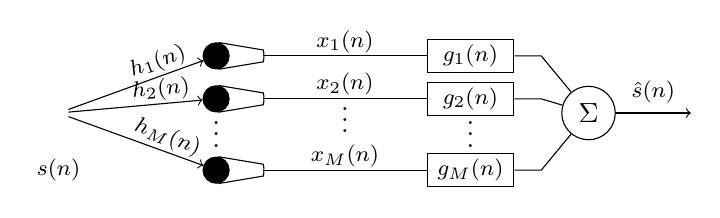
\begin{tikzpicture}
    % Adjustments
    \def\micd{.1cm}                % mic diameter
    \def\micl{.6cm}                % mic length
    \def\micw{.15cm}               % mic width
    \def\micbend{10}               % mic bottom bend
    \def\micdistance{.2cm}         % distance between microphones
    \def\filterdistance{2.5cm}     % distance between microphone and filter
    \def\filteroutline{.9cm}       % length of line which gets out of filter
    \def\sumdistance{1.5cm}        % distance of sum node to the filter
    \def\sumoutline{1cm}           % length of line which gets out of sum
    \def\headdistance{2cm}         % distance between microphone and head

    % Styles
    \tikzset{%
      mic head/.style={fill=black,draw=black,circle,minimum size=\micd},
      filter/.style={draw,minimum width=1.1cm,inner sep=2pt},
      sum/.style={draw,circle},
      xlabel/.style={inner sep=1pt,above,midway},
      sumlabel/.style={xlabel},
      hlabel/.style={xlabel,sloped,pos=.7},
      head/.style={font=\Large}
    }

    % Draw Microphones
    \begin{scope}[start chain=going below,every node/.style={on chain},node distance=\micdistance]
      \node[mic head] (mic1) {};
      \node[mic head] (mic2) {};
      \node[mic head,yshift=-1.8*\micdistance] (mic3) {};
    \end{scope}
    \node[yshift=3pt] at ($(mic2)!.5!(mic3)$) {$\vdots$};

    \foreach \m in {1,2,3} {%
      \coordinate (m1) at ($(mic\m)+(\micl,\micw/2)$);
      \coordinate (m2) at ($(mic\m)+(\micl,-\micw/2)$);
      \draw (tangent cs:node=mic\m,point={(m1)},solution=1) -- (m1) to[bend left=\micbend] (m2) -- (tangent cs:node=mic\m,point={(m2)},solution=2);
    }

    % Draw Filter
    \foreach \m/\i in {1/1,2/2,3/M} {%
      \node[filter,right=\filterdistance of mic\m] (filter\m) {\footnotesize $g_{\i}(n)$};
      \draw ($(mic\m)+(\micl,0)$) to node[xlabel] (x\m) {\footnotesize $x_{\i}(n)$} (filter\m);
    }
    \node[yshift=3pt] at ($(filter2)!.5!(filter3)$) {$\vdots$};
    \node[yshift=3pt] at ($(x2)!.5!(x3)$) {$\vdots$};
    % Sum Node
    \node[sum] (sum) at ($(filter1)!.5!(filter3)+(\sumdistance,0)$) {$\Sigma$};
    \draw[->] (sum) -- node[above] {\footnotesize $\hat{s}(n)$} ++(1.3,0);
    % Connect filter with sum
    \foreach \m in {1,2,3} {%
      \draw (filter\m) -- ++(\filteroutline,0) -- (sum);
    }

    % Head
    \node[head] (head) at ($(mic1)!.5!(mic3)-(\headdistance,0)$) {\PHtattooedHead};
    \node[fill=white,minimum width=4.8pt,minimum height=5.7pt,inner sep=0pt] at ($(head.center)+(2.3pt,-2.5pt)$) {};
    \node at ($(head.center)+(0.0pt,-20.5pt)$) {\footnotesize $s(n)$};
    % Connect head with mics
    \foreach \m/\i in {1/1,2/2,3/M} {%
      \draw[->] (head) -- node[hlabel] {\footnotesize $h_{\i}(n)$} (mic\m);
    }
  \end{tikzpicture}
  \caption{Multichannel equalization system}
  \label{fig: acsys}
\end{figure}

\noindent The RIR can be described in vector notation as $\mathbf{h}_m = [h_m(0) \; h_m(1) \; \ldots \; h_m(L_h-1)]^T$, with $L_h$ being the RIR length and $[\cdot]^T$ denoting the transpose operation.
Equalization techniques design and apply reshaping filters $\mathbf{g}_m$ of length $L_g$, i.e. $\mathbf{g}_m = [g_m(0) \; g_m(1) \; \ldots \; g_m(L_g-1)]^T$, yielding the output signal
\begin{equation}
  \small
  \hat{s}(n)  = \sum_{m=1}^M x_m(n) \ast g_m(n) =  s(n) \ast \underbrace{\sum_{m=1}^M h_m(n) \ast g_m(n)}_{c(n)},
\end{equation}
where $c(n)$ denotes the equalized impulse response~(EIR) of length $L_c = L_h+L_g-1$, i.e. $\mathbf{c} = [c(0) \; c(1) \; \ldots \; c(L_c-1)]^T$.
Using the stacked $ML_g$-dimensional reshaping filter $\mathbf{g}$ and the $L_c \times ML_g$-dimensional multichannel convolution matrix $\mathbf{H}$, i.e.
\begin{eqnarray}
  \mathbf{g} &=& [\mathbf{g}_1^T \; \mathbf{g}_2^T \; \ldots \; \mathbf{g}_M^T]^T, \\
  \mathbf{H} &=& [\mathbf{H}_1 \; \mathbf{H}_2 \; \ldots \; \mathbf{H}_M],
\end{eqnarray}
with $\mathbf{H}_m$ being the $L_c \times L_g$-dimensional convolution matrix of $\mathbf{h}_m$, the EIR can be expressed as
\begin{equation}
  \label{eq: trueeir}
  \boxed{\mathbf{c} = \mathbf{H} \mathbf{g}}
\end{equation}
The reshaping filter $\mathbf{g}$ can then be designed based on different optimization criteria for the EIR $\mathbf{c}$.
When the RIRs do not share any common zeros and the reshaping filter length is $L_g \geq \lceil \frac{L_h-1}{M-1}\rceil$, the EIR can be perfectly reshaped to a desired target response~\cite{Kodrasi_ITASLP_2013,Miyoshi_ITASS_1988}.
Since the true RIRs are however generally not available in practice~\cite{Hasan_EUSIPCO_2006}, acoustic multichannel equalization techniques design $\mathbf{g}$ using the estimated multichannel convolution matrix $\hat{\mathbf{H}}$~(constructed from the estimated RIRs $\hat{\mathbf{h}}_m$).
Several techniques which aim at decreasing the sensitivity of $\mathbf{g}$ to RIR estimation errors have been proposed, of which the P-MINT, RMCLS-CIT, CS, and PeCCS techniques are briefly reviewed in the following.

\textit{Partial Multichannel Equalization Based on the Multiple-Input/Output Inverse Theorem}~\cite{Kodrasi_ITASLP_2013}. \enspace
P-MINT aims at designing a reshaping filter that simultaneously sets the reverberant tail of the EIR to $\mathbf{0}$ and preserves the perceptual speech quality.
This objective is formulated as the minimization of the least-squares cost function
\begin{equation}
\label{eq: pmintcost}
\boxed{J_{_{\rm P-MINT}} = \|\hat{\mathbf{H}}\mathbf{g} - \hat{\mathbf{h}}_p^{\rm d}\|_2^2}
\end{equation}
where the target EIR is chosen to be equal to $\hat{\mathbf{h}}_p^{\rm d}$, which denotes the first part~(i.e. direct path and early reflections) of one of the estimated RIRs, i.e.
\begin{equation}
\hat{\mathbf{h}}_{p}^{\rm d} = [\underbrace{0\phantom{\rlap{$(L_d-1)$}} \ldots 0 }_{\tau} \underbrace{\hat{h}_p(0) \ldots \hat{h}_p(L_d-1)}_{L_d} 0 \ldots 0 ]^{T},
\end{equation}
with $\tau$ a delay, $L_d$ the length of the direct path and early reflections, and $p \in \{1, \; \ldots, \; M\}$.
In order to increase the robustness of P-MINT to errors in the estimated RIRs, a regularization term has been incorporated, leading to the regularized P-MINT cost function
\begin{equation}
  \label{eq: rpmintcost}
  \boxed{J_{_{\rm P-MINT}}^{{\rm R}} = \|\hat{\mathbf{H}}\mathbf{g} - \hat{\mathbf{h}}_p^{\rm d}\|_2^2 + \delta \|\mathbf{g}\|_2^2}
\end{equation}
with $\delta$ being a regularization parameter.
The regularized P-MINT reshaping filter minimizing~(\ref{eq: rpmintcost}) can be computed as
\begin{equation}
  \label{eq: rpmintsol}
  \boxed{\mathbf{g}_{_{\rm P-MINT}}^{{\rm R}} = (\hat{\mathbf{H}}^T\hat{\mathbf{H}}+\delta \mathbf{I})^{-1} \hat{\mathbf{H}}^T \hat{\mathbf{h}}_p^{\rm d}}
\end{equation}
with $\mathbf{I}$ being the $ML_g \times ML_g$-dimensional identity matrix.

\textit{Relaxed Multichannel Least Squares with Constrained Initial Taps}~\cite{Lim_IWAENC_2012}. \enspace
RMCLS-CIT aims at setting the reverberant tail of the EIR to $\mathbf{0}$, while partly controlling the perceptual speech quality.
This can be achieved by introducing a weighting matrix $\mathbf{W}_{r}$ in the least-squares cost function in~(\ref{eq: pmintcost}), i.e.
\begin{equation}
  \label{eq: rmclscitcost}
  \boxed{J_{_{\rm RMCLS-CIT}} = \|\mathbf{W}_{r}(\hat{\mathbf{H}}\mathbf{g} - \hat{\mathbf{h}}_p^{\rm d})\|_2^2}
\end{equation}
with
\begin{equation}
\label{eq: wrmclscit}
\mathbf{W}_{r} = \diag\{[\underbrace{1 \; \ldots \; 1}_{\tau} \; \underbrace{1 \; \ldots \; 1}_{L_r} \underbrace{0 \; \ldots \; 0}_{L_d-L_r} \; 1 \; \ldots 1]\},
\end{equation}
where $L_r$ denotes the number of initial taps to be constrained within the desired window length.
Since it has been shown that regularization increases the robustness of equalization techniques to RIR estimation errors~\cite{Kodrasi_ITASLP_2013}, we introduce a regularization term in the RMCLS-CIT cost function in~(\ref{eq: rmclscitcost}), leading to the regularized RMCLS-CIT cost function
\begin{equation}
  \label{eq: rrmclscitcost}
  \boxed{J_{_{\rm RMCLS-CIT}}^{{\rm R}} = \|\mathbf{W}_{r}(\hat{\mathbf{H}}\mathbf{g} - \hat{\mathbf{h}}_p^{\rm d})\|_2^2 + \delta \|\mathbf{g}\|_2^2}
\end{equation}
The reshaping filter minimizing the regularized least-squares cost function in~(\ref{eq: rrmclscitcost}) can be computed as
\begin{empheq}[box=\fbox]{align}
   \mathbf{g}_{_{\rm RMCLS-CIT}}^{\rm R} & = [(\mathbf{W}_{r} \hat{\mathbf{H}})^T(\mathbf{W}_{r} \hat{\mathbf{H}}) + \delta \mathbf{I}]^{-1} \nonumber  \\
  & \times (\mathbf{W}_{r} \hat{\mathbf{H}})^T (\mathbf{W}_{r}\hat{\mathbf{h}}_p^{\rm d})
\end{empheq}

\textit{Channel Shortening}~\cite{Zhang_IWAENC_2010, Kallinger_ICASSP_2006}. \enspace
The objective of CS is to maximize the energy ratio between the first $L_d$ taps~(i.e. direct path and early reflections) and the remaining taps~(i.e. reverberant tail) of the EIR without imposing further constraints on the perceptual speech quality.
This objective is expressed in terms of a generalized Rayleigh quotient maximization problem, i.e.
\begin{equation}
  \label{eq: cscost}
  \boxed{J_{_{\rm CS}} = \frac{\|\mathbf{W}_d \hat{\mathbf{H}}\mathbf{g} \|_2^2}{\|\mathbf{W}_u \hat{\mathbf{H}}\mathbf{g} \|_2^2} = \frac{\mathbf{g}^T\hat{\mathbf{B}}\mathbf{g}}{\mathbf{g}^T\hat{\mathbf{A}}\mathbf{g}}}
\end{equation}
with
\begin{align}
\label{eq: wincs}
\mathbf{W}_d & = {\diag} \{ [\underbrace{0 \; \ldots \; 0}_{\tau} \; \underbrace{1 \; \ldots \; 1}_{L_d}\; 0\; \ldots\; 0] \},  \\
\mathbf{W}_u & =  {\diag} \{ [\underbrace{1 \; \ldots \; 1}_{\tau} \; \underbrace{0 \; \ldots \; 0}_{L_d}\; 1\; \ldots\; 1] \},
\end{align}
and
\begin{align}
\hat{\mathbf{B}} & = \hat{\mathbf{H}}^{T} \mathbf{W}_d^T\mathbf{W}_d\hat{\mathbf{H}},  \\
\hat{\mathbf{A}} & = \hat{\mathbf{H}}^{T}\mathbf{W}_u^T\mathbf{W}_u \hat{\mathbf{H}}.
\end{align}
Maximizing~(\ref{eq: cscost}) is equivalent to solving the generalized eigenvalue problem $\hat{\mathbf{B}}\mathbf{g} = \lambda \hat{\mathbf{A}}\mathbf{g}$, where the optimal reshaping filter $\mathbf{g}_{_{\rm CS}}$ is the generalized eigenvector corresponding to the largest generalized eigenvalue $\lambda_{\max}$, i.e.
\begin{equation}
  \label{eq: cssol}
  \boxed{\hat{\mathbf{B}}\mathbf{g}_{_{\rm CS}} = \lambda_{\max}\hat{\mathbf{A}}\mathbf{g}_{_{\rm CS}}}
\end{equation}
In~\cite{Zhang_IWAENC_2010} it has been shown that there exist $L_d$ linearly independent generalized eigenvectors $\mathbf{g}_{_{\rm CS}}^1, \; \mathbf{g}_{_{\rm CS}}^2, \; \ldots \; \mathbf{g}_{_{\rm CS}}^{L_d},$ satisfying~(\ref{eq: cssol}), which however yield a different performance in terms of reverberant energy suppression and perceptual speech quality.
Following similar arguments as in~\cite{Zhang_IWAENC_2010} it can be shown that the reshaping filters computed by P-MINT and RMCLS-CIT also satisfy $\mathbf{g}^{T}\hat{\mathbf{A}}\mathbf{g} = 0$ and $\mathbf{g}^{T}\hat{\mathbf{B}}\mathbf{g} \neq 0$, such that they also maximize the generalized Rayleigh quotient in~(\ref{eq: cscost}).
Hence, the solutions to the P-MINT and the RMCLS-CIT cost functions in~(\ref{eq: pmintcost}) and~(\ref{eq: rmclscitcost}) can be expressed as linear combinations of the multiple CS generalized eigenvectors\footnote{The proof of this statement is omitted due to space constraints.}.

{\textit{Perceptually Constrained Channel Shortening}}~\cite{Kodrasi_ICASSP_2013}. \enspace
PeCCS aims at resolving the selection ambiguity of CS by finding a linear combination of the multiple CS reshaping filters that leads to the P-MINT target response.
The linear combination $\boldsymbol \alpha$ is found by minimizing the cost function
\begin{equation}
\label{eq: peccscost}
 \boxed{J_{_{\rm PeCCS}} =  \|\hat{\mathbf{H}}\mathbf{G} \boldsymbol \alpha - \hat{\mathbf{h}}_p^{\rm d} \|_2^2 + \|\mathbf{G} \boldsymbol \alpha \|_2^2}
\end{equation}
with $\mathbf{G} = [\mathbf{g}_{_{\rm CS}}^1 \; \mathbf{g}_{_{\rm CS}}^2 \; \ldots \mathbf{g}_{_{\rm CS}}^{L_d}] $ being an $ML_g \times L_d$-dimensional matrix whose columns span the solution space of CS.
Minimizing~(\ref{eq: peccscost}) yields the linear combination vector
\begin{equation}
\boxed{\boldsymbol \alpha_{_{\rm PeCCS}}  = [(\hat{\mathbf{H}}\mathbf{G})^T(\hat{\mathbf{H}}\mathbf{G}) + \mathbf{G}^T\mathbf{G}]^{-1}  (\hat{\mathbf{H}}\mathbf{G})^T \hat{\mathbf{h}}_p^{\rm d}}
\end{equation}
leading to the PeCCS reshaping filter
\begin{equation}
  \label{eq: peccssol}
  \boxed{\mathbf{g}_{_{\rm PeCCS}} = \mathbf{G} \boldsymbol \alpha_{_{\rm PeCCS}}}
\end{equation}
In the following, we propose extending the PeCCS technique through incorporating regularization and a weighting matrix in order to further increase robustness to channel estimation errors.

% In the following we propose a novel method for computing a perceptually advantageous reshaping filter as a robust linear combinations of the generalized eigenvectors satisfying~(\ref{eq: cssol}).

\vspace{-0.25cm}
\section{Regularized Subspace-Based Acoustic Multichannel Equalization}
\vspace{-0.25cm}

% Consider the subspace $\mathcal{S}_{\rm CS}$ of $ML_g$-dimensional vectors spanned by the $L_d$ generalized eigenvectors maximizing~(\ref{eq: cscost}).
% Clearly any linear combination of these generalized eigenvectors, i.e.
% \begin{equation}
% \mathbf{g} = \mathbf{G} \boldsymbol \alpha \in \mathcal{S}_{\rm CS}
% \end{equation}
% with $\mathbf{G} = [\mathbf{g}_{\rm CS}^1 \; \mathbf{g}_{\rm CS}^2 \; \ldots \mathbf{g}_{\rm CS}^{L_d}] $ and $\boldsymbol \alpha$ being an $L_d$-dimensional vector of scalar coefficients, leads to a reshaping filter which also maximizes~(\ref{eq: cscost}).
In~\cite{Kodrasi_ITASLP_2013} it has been experimentally validated that there exist reshaping filters in the solution space of CS which can achieve a high level of reverberant tail suppression. 
In order to obtain a robust reshaping filter in this solution space which also yields perceptual speech quality preservation, we propose the regularized subspace-based cost function~(SuB) 
\begin{equation}
\label{eq: subcost}
\boxed{J_{\rm SuB}^{\rm R} = \|\mathbf{W}(\hat{\mathbf{H}}\mathbf{G}\boldsymbol \alpha - \hat{\mathbf{h}}_p^{\rm d})\|_2^2 + \delta \|\mathbf{G} \boldsymbol \alpha \|_2^2}
\end{equation}
with $\mathbf{W}$ being an $L_c \times L_c$-dimensional weighting matrix.
The first term in~(\ref{eq: subcost}) aims at finding a linear combination of the generalized eigenvectors that yields the perceptually advantageous desired target response $\hat{\mathbf{h}}_p^{\rm d}$.
Using a weighting matrix $\mathbf{W} \neq \mathbf{I}$ allows to relax the constraints on the reshaping filter design, which may increase robustness in the presence of RIR estimation errors.
The second term in~(\ref{eq: subcost}) controls the reshaping filter energy by means of the regularization parameter $\delta$, in order to avoid distortions in the output signal due to errors in the estimated RIRs.

The vector $\boldsymbol \alpha_{\rm SuB}^{\rm R}$ minimizing~(\ref{eq: subcost}) is given by
\begin{empheq}[box=\fbox]{align}
   \boldsymbol \alpha_{\rm SuB}^{\rm R} & = [(\mathbf{W} \hat{\mathbf{H}} \mathbf{G})^T(\mathbf{W} \hat{\mathbf{H}} \mathbf{G}) + \delta \mathbf{G}^T \mathbf{G}]^{-1} \nonumber  \\
  & \times (\mathbf{W}\hat{\mathbf{H}} \mathbf{G})^T (\mathbf{W} \hat{\mathbf{h}}_p^{\rm d})
\end{empheq}
leading to the reshaping filter
\begin{equation}
\boxed{\mathbf{g}_{\rm SuB}^{\rm R} = \mathbf{G} \boldsymbol \alpha_{\rm SuB}^{\rm R}}
\end{equation}
Depending on the choice of $\mathbf{W}$ and $\delta$, the cost function in~(\ref{eq: subcost}) gives rise to different reshaping filters.
When regularization is omitted, i.e. $\delta = 0$, two special cases can be considered: 1) when $\mathbf{W} = \mathbf{I}$, the obtained reshaping filter minimizes the P-MINT cost function in~(\ref{eq: pmintcost}); 2) when $\mathbf{W} = \mathbf{W}_{r}$, the obtained reshaping filter minimizes the RMCLS-CIT cost function in~(\ref{eq: rmclscitcost}).
Furthermore, with $\delta = 1$ and $\mathbf{W} = \mathbf{I}$, minimizing~(\ref{eq: subcost}) yields the PeCCS reshaping filter in~(\ref{eq: peccssol}).

In the following, the performance of the regularized SuB technique for $\delta \neq 0$ is investigated for two different scenarios: 1) using no weighting matrix, i.e. $\mathbf{W} = \mathbf{I}$; 2) using the RMCLS-CIT weighting matrix, i.e. $\mathbf{W} = \mathbf{W}_{r}$ defined in~(\ref{eq: wrmclscit}).

\vspace{-0.25cm}
\section{Experimental Results}
\vspace{-0.25cm}

In order to investigate the performance of the proposed technique, we have considered a measured acoustic system with $M = 2$ microphones in a room with reverberation time $T_{\rm 60} \approx 700$~ms as the true system to be equalized.
The sampling frequency is $f_s = 8$~kHz, the RIR length is $L_h = 3000$, and $5$ different desired window lengths are investigated, i.e. $L_w \in \{ 10~{\rm ms}, 20~{\rm ms}, 30~{\rm ms}, 40~{\rm ms}, 50~{\rm ms} \}$, with $L_w = \frac{L_d \times 10^3}{f_s}$ being the desired window length in ms.
Furthermore, the simulation parameters are set to $\tau = 0$, $L_g = 2999$, $p=1$, and $L_r = \lfloor \frac{L_d}{3} \rfloor$.

In order to simulate estimation errors, the true acoustic system is perturbed as in~\cite{Cho_ITSA_1999}, i.e.
\begin{equation}
\hat{h}_m(n) = h_m(n)[1 + e_m(n)],
\end{equation}
with $e_m(n)$ being an uncorrelated Gaussian noise sequence with zero mean and an appropriate variance, such that a normalized channel mismatch $E_m$, defined as
\begin{equation}
  E_m = 10 \log_{10} \frac{\|\mathbf{h}_m-\hat{\mathbf{h}}_m\|_2^2}{\|\mathbf{h}_m\|_2^2},
\end{equation}
is generated.
The considered normalized channel mismatch values are $E_m = -33$~dB and $E_m = -24$~dB.
\begin{figure}[b!]
  % This file was created by matlab2tikz v0.4.0.
% Copyright (c) 2008--2013, Nico Schlömer <nico.schloemer@gmail.com>
% All rights reserved.
% 
% The latest updates can be retrieved from
%   http://www.mathworks.com/matlabcentral/fileexchange/22022-matlab2tikz
% where you can also make suggestions and rate matlab2tikz.
% 
% 
% 

% defining custom colors
\definecolor{mycolor1}{rgb}{0,0.75,0.75}%
\definecolor{mycolor2}{rgb}{0.75,0,0.75}%
\definecolor{mycolor3}{rgb}{0.75,0.75,0}%

\begin{tikzpicture}[font = \small]

\begin{axis}[%
width=\figurewidth,
height=\figureheight,
scale only axis,
xmin=0,
xmax=400,
xlabel={Time [ms]},
xlabel absolute, xlabel style={yshift=0.5em},
xmajorgrids,
ymin=-50,
ymax=0,
ylabel={EDC [dB]},
ylabel absolute, ylabel style={yshift=-0.8em},
ymajorgrids,
legend style={at={(0.99,0.99)},draw=black,fill=white,legend cell align=left, row sep = -4pt}
]

\addlegendimage{blue, line width = 1.2, mark = o, mark size=1.8pt};
\addlegendentry{P- MINT};
\addlegendimage{color=green!50!black, line width = 1.2pt,mark = square, mark size=1.8pt};
\addlegendentry{RMCLS-CIT};
\addlegendimage{color=mycolor1, solid, line width = 3pt};
\addlegendentry{SuB ($\mathbf{W} = \mathbf{I}$)};
\addlegendimage{color=black, solid, line width = 1.5pt};
\addlegendentry{SuB ($\mathbf{W} = \mathbf{W}_r$)};
\addlegendimage{black, line width = 1.5pt, dashed};
\addlegendentry{$\mathbf{h}_1$};


\addplot [
color=blue,
solid,
line width=1.2pt
]
table[row sep=crcr]{
0 0\\
5.00083375020844 -0.455190706619499\\
10.0016675004169 -1.0728438645242\\
15.0025012506253 -1.74026774895808\\
20.0033350008338 -2.6912641547612\\
25.0041687510422 -4.62120927713282\\
30.0050025012506 -6.19397879234129\\
35.0058362514591 -7.67506557963489\\
40.0066700016675 -9.42236458923914\\
45.0075037518759 -13.0241338880517\\
50.0083375020844 -25.4114385013253\\
55.0091712522928 -25.6282278745616\\
60.0100050025013 -25.7801472550873\\
65.0108387527097 -25.8718112735296\\
70.0116725029181 -25.9801235972093\\
75.0125062531266 -26.2130983444718\\
80.013340003335 -26.4184617428363\\
85.0141737535434 -26.6007550762732\\
90.0150075037519 -26.8273560454276\\
95.0158412539603 -27.0859206614555\\
100.016675004169 -27.1740312495137\\
105.017508754377 -27.3125017963358\\
110.018342504586 -27.5050405136709\\
115.019176254794 -27.7070947135801\\
120.020010005003 -27.9832756195885\\
125.020843755211 -28.116875880641\\
130.021677505419 -28.2446329686554\\
135.022511255628 -28.3478199283342\\
140.023345005836 -28.5571065071029\\
145.024178756045 -28.6618507720671\\
150.025012506253 -28.747798756242\\
155.025846256462 -28.8710075422229\\
160.02668000667 -29.0202587637674\\
165.027513756878 -29.2343437163966\\
170.028347507087 -29.4043439708216\\
175.029181257295 -29.5224609357927\\
180.030015007504 -29.6217513246874\\
185.030848757712 -29.7786300070902\\
190.031682507921 -29.9052392352347\\
195.032516258129 -30.093506025237\\
200.033350008337 -30.2808488771748\\
205.034183758546 -30.3828880904571\\
210.035017508754 -30.4938129835039\\
215.035851258963 -30.6010473871189\\
220.036685009171 -30.76103446653\\
225.03751875938 -30.8486837768002\\
230.038352509588 -31.0560629761081\\
235.039186259797 -31.2839637994546\\
240.040020010005 -31.4808987088516\\
245.040853760213 -31.5654921026252\\
250.041687510422 -31.7136588473268\\
255.04252126063 -31.8880410980501\\
260.043355010839 -31.9579965561513\\
265.044188761047 -32.0391032512669\\
270.045022511256 -32.210447214156\\
275.045856261464 -32.3206245137548\\
280.046690011673 -32.5606000612963\\
285.047523761881 -32.6652019007627\\
290.048357512089 -32.7725072769753\\
295.049191262298 -32.897225410048\\
300.050025012506 -33.0185434552216\\
305.050858762715 -33.1778946249492\\
310.051692512923 -33.3055499659283\\
315.052526263132 -33.4967625203025\\
320.05336001334 -33.7148285777713\\
325.054193763548 -33.8091655832599\\
330.055027513757 -33.9531396332191\\
335.055861263965 -34.0511350896133\\
340.056695014174 -34.1629734687773\\
345.057528764382 -34.409772602393\\
350.058362514591 -34.7375546100135\\
355.059196264799 -34.9034833911641\\
360.060030015008 -35.0300446440915\\
365.060863765216 -35.0987871361508\\
370.061697515424 -35.1371769411295\\
375.062531265633 -35.2045676671675\\
380.063365015841 -35.3527747518678\\
385.06419876605 -35.4234751024016\\
390.065032516258 -35.5290410372038\\
395.065866266467 -35.6999139068032\\
400.066700016675 -35.8224990471287\\
};
\addplot [
color=blue,
line width=1.2pt,
mark size=1.8pt,
only marks,
mark=o,
mark options={solid}
]
table[row sep=crcr]{
0 0\\
15.0025012506253 -1.74026774895808\\
30.0050025012506 -6.19397879234129\\
45.0075037518759 -13.0241338880517\\
60.0100050025013 -25.7801472550873\\
75.0125062531266 -26.2130983444718\\
90.0150075037519 -26.8273560454276\\
105.017508754377 -27.3125017963358\\
120.020010005003 -27.9832756195885\\
135.022511255628 -28.3478199283342\\
150.025012506253 -28.747798756242\\
165.027513756878 -29.2343437163966\\
180.030015007504 -29.6217513246874\\
195.032516258129 -30.093506025237\\
210.035017508754 -30.4938129835039\\
225.03751875938 -30.8486837768002\\
240.040020010005 -31.4808987088516\\
255.04252126063 -31.8880410980501\\
270.045022511256 -32.210447214156\\
285.047523761881 -32.6652019007627\\
300.050025012506 -33.0185434552216\\
315.052526263132 -33.4967625203025\\
330.055027513757 -33.9531396332191\\
345.057528764382 -34.409772602393\\
360.060030015008 -35.0300446440915\\
375.062531265633 -35.2045676671675\\
390.065032516258 -35.5290410372038\\
};
\addplot [
color=green!50!black,
line width=1.2pt
]
table[row sep=crcr]{
0 0\\
5.00083375020844 -0.393249381656358\\
10.0016675004169 -0.905501406679307\\
15.0025012506253 -1.44905489692544\\
20.0033350008338 -2.30237966456518\\
25.0041687510422 -3.79436322419237\\
30.0050025012506 -4.98848361023411\\
35.0058362514591 -6.48893706891077\\
40.0066700016675 -8.72212797245803\\
45.0075037518759 -11.4627956121562\\
50.0083375020844 -28.0625980432118\\
55.0091712522928 -28.2459955819667\\
60.0100050025013 -28.4181296009636\\
65.0108387527097 -28.5137648226726\\
70.0116725029181 -28.712070196084\\
75.0125062531266 -29.0064072524928\\
80.013340003335 -29.1724243075495\\
85.0141737535434 -29.4001131254397\\
90.0150075037519 -29.6364003137508\\
95.0158412539603 -29.8362965614707\\
100.016675004169 -29.9296898409669\\
105.017508754377 -30.1121985359925\\
110.018342504586 -30.4437599358158\\
115.019176254794 -30.7844576738392\\
120.020010005003 -31.0962180520178\\
125.020843755211 -31.2983999557701\\
130.021677505419 -31.3972694805218\\
135.022511255628 -31.511185902992\\
140.023345005836 -31.639815730116\\
145.024178756045 -31.7513791396288\\
150.025012506253 -31.8450058669331\\
155.025846256462 -31.9066297269722\\
160.02668000667 -32.0358412210064\\
165.027513756878 -32.3051766743465\\
170.028347507087 -32.5213128258442\\
175.029181257295 -32.5955063094394\\
180.030015007504 -32.7054066244066\\
185.030848757712 -32.8475776339947\\
190.031682507921 -33.0215329364891\\
195.032516258129 -33.2156695182545\\
200.033350008337 -33.3796435018557\\
205.034183758546 -33.5652760706672\\
210.035017508754 -33.7286748866152\\
215.035851258963 -34.0770270903827\\
220.036685009171 -34.1796310735902\\
225.03751875938 -34.3599092827419\\
230.038352509588 -34.8750249468909\\
235.039186259797 -35.3581689406989\\
240.040020010005 -35.6515324479463\\
245.040853760213 -35.823683873883\\
250.041687510422 -35.9372573090514\\
255.04252126063 -36.0245064579546\\
260.043355010839 -36.171909904239\\
265.044188761047 -36.290147107032\\
270.045022511256 -36.4048533319223\\
275.045856261464 -36.5196461527588\\
280.046690011673 -36.9865267694024\\
285.047523761881 -37.1327498479191\\
290.048357512089 -37.4913864582665\\
295.049191262298 -37.7905543266338\\
300.050025012506 -38.1187335540777\\
305.050858762715 -38.8360496652457\\
310.051692512923 -39.059894250721\\
315.052526263132 -39.5520457532561\\
320.05336001334 -39.8305525203838\\
325.054193763548 -39.9397001800984\\
330.055027513757 -40.18315811164\\
335.055861263965 -40.2933823002098\\
340.056695014174 -40.4456260720553\\
345.057528764382 -40.5901928818296\\
350.058362514591 -40.9207074581369\\
355.059196264799 -41.0748238171529\\
360.060030015008 -41.4863440651505\\
365.060863765216 -41.6547384625949\\
370.061697515424 -41.7944407450833\\
375.062531265633 -41.9268298903579\\
380.063365015841 -42.0835195828015\\
385.06419876605 -42.2794650047943\\
390.065032516258 -42.6336739571495\\
395.065866266467 -43.281458193116\\
400.066700016675 -43.7816184992539\\
};
\addplot [
color=green!50!black,
line width=1.2pt,
only marks,
mark=square,
mark size=1.8pt,
mark options={solid},
forget plot
]
table[row sep=crcr]{
0 0\\
15.0025012506253 -1.44905489692544\\
30.0050025012506 -4.98848361023411\\
45.0075037518759 -11.4627956121562\\
60.0100050025013 -28.4181296009636\\
75.0125062531266 -29.0064072524928\\
90.0150075037519 -29.6364003137508\\
105.017508754377 -30.1121985359925\\
120.020010005003 -31.0962180520178\\
135.022511255628 -31.511185902992\\
150.025012506253 -31.8450058669331\\
165.027513756878 -32.3051766743465\\
180.030015007504 -32.7054066244066\\
195.032516258129 -33.2156695182545\\
210.035017508754 -33.7286748866152\\
225.03751875938 -34.3599092827419\\
240.040020010005 -35.6515324479463\\
255.04252126063 -36.0245064579546\\
270.045022511256 -36.4048533319223\\
285.047523761881 -37.1327498479191\\
300.050025012506 -38.1187335540777\\
315.052526263132 -39.5520457532561\\
330.055027513757 -40.18315811164\\
345.057528764382 -40.5901928818296\\
360.060030015008 -41.4863440651505\\
375.062531265633 -41.9268298903579\\
390.065032516258 -42.6336739571495\\
};
\addplot [
color=mycolor1,
solid,
line width=3.0pt,
forget plot
]
table[row sep=crcr]{
0 0\\
5.00083375020844 -0.191207206703132\\
10.0016675004169 -0.324276698917874\\
15.0025012506253 -0.651608315867823\\
20.0033350008338 -1.24655684882357\\
25.0041687510422 -2.45732165166562\\
30.0050025012506 -4.20265721841769\\
35.0058362514591 -5.83515516589665\\
40.0066700016675 -8.58193490176338\\
45.0075037518759 -12.5753056948167\\
50.0083375020844 -29.6857709529958\\
55.0091712522928 -29.8202839283848\\
60.0100050025013 -30.0530023860964\\
65.0108387527097 -30.2345407080685\\
70.0116725029181 -30.4308068623878\\
75.0125062531266 -30.7373225816511\\
80.013340003335 -31.1916988365486\\
85.0141737535434 -31.3970693868681\\
90.0150075037519 -31.6114948865535\\
95.0158412539603 -31.8969292978797\\
100.016675004169 -32.1750629870584\\
105.017508754377 -32.5561602833086\\
110.018342504586 -33.0196565259675\\
115.019176254794 -33.3422184774516\\
120.020010005003 -33.5838576946574\\
125.020843755211 -33.8195467850323\\
130.021677505419 -34.226626439758\\
135.022511255628 -34.5353228837757\\
140.023345005836 -34.8166657985356\\
145.024178756045 -35.1398669694776\\
150.025012506253 -35.423172808542\\
155.025846256462 -35.8390838280628\\
160.02668000667 -36.0562727575327\\
165.027513756878 -36.3343051624008\\
170.028347507087 -36.8015542312618\\
175.029181257295 -37.0835354135813\\
180.030015007504 -37.3871581026732\\
185.030848757712 -37.8193221504036\\
190.031682507921 -38.1791251335016\\
195.032516258129 -38.5894143251941\\
200.033350008337 -38.8630904871338\\
205.034183758546 -39.1147133409059\\
210.035017508754 -39.3816136725189\\
215.035851258963 -39.604931526592\\
220.036685009171 -40.0103666031628\\
225.03751875938 -40.1865901643736\\
230.038352509588 -40.6183975530405\\
235.039186259797 -41.0650785001543\\
240.040020010005 -41.479677717525\\
245.040853760213 -41.7996417516278\\
250.041687510422 -42.1203150699362\\
255.04252126063 -42.4621498484439\\
260.043355010839 -42.7296927630691\\
265.044188761047 -43.1376052995004\\
270.045022511256 -43.5566175042857\\
275.045856261464 -44.202379555675\\
280.046690011673 -44.3940024134497\\
285.047523761881 -44.8308711655591\\
290.048357512089 -45.4799430997554\\
295.049191262298 -46.0506907141554\\
300.050025012506 -46.4074286076447\\
305.050858762715 -46.7395614741197\\
310.051692512923 -46.9129015505164\\
315.052526263132 -47.157446754327\\
320.05336001334 -47.6358252033723\\
325.054193763548 -47.7679752838492\\
330.055027513757 -48.1948525442126\\
335.055861263965 -48.5269321046474\\
340.056695014174 -48.9572360321987\\
345.057528764382 -49.1525730045571\\
350.058362514591 -49.4817366018574\\
355.059196264799 -49.9485462610217\\
360.060030015008 -50.592455548977\\
};
\addplot [
color=black,
solid,
line width=1.5pt,
forget plot
]
table[row sep=crcr]{
0 0\\
5.00083375020844 -0.196539645001274\\
10.0016675004169 -0.584475162968716\\
15.0025012506253 -1.73313060928351\\
20.0033350008338 -2.4885826072818\\
25.0041687510422 -3.28208853454639\\
30.0050025012506 -4.86513346198432\\
35.0058362514591 -7.00470096137261\\
40.0066700016675 -9.31704989341585\\
45.0075037518759 -13.8932263584153\\
50.0083375020844 -30.8240368446172\\
55.0091712522928 -31.0317908145847\\
60.0100050025013 -31.2730211795714\\
65.0108387527097 -31.4745331290358\\
70.0116725029181 -31.720259587169\\
75.0125062531266 -32.0632094017818\\
80.013340003335 -32.4756068671243\\
85.0141737535434 -32.7273706911838\\
90.0150075037519 -33.0323761011966\\
95.0158412539603 -33.2953075474401\\
100.016675004169 -33.5611461288815\\
105.017508754377 -33.7450091290279\\
110.018342504586 -34.0011620071551\\
115.019176254794 -34.4621819366376\\
120.020010005003 -34.690720636024\\
125.020843755211 -34.9695013198564\\
130.021677505419 -35.1557860044584\\
135.022511255628 -35.4193311630929\\
140.023345005836 -35.6980145827992\\
145.024178756045 -35.9554483009108\\
150.025012506253 -36.1742001637372\\
155.025846256462 -36.5160226312554\\
160.02668000667 -36.8475164485312\\
165.027513756878 -37.1477797142213\\
170.028347507087 -37.56968189029\\
175.029181257295 -37.8496892019654\\
180.030015007504 -38.1847275122608\\
185.030848757712 -38.8206674375064\\
190.031682507921 -39.146355251939\\
195.032516258129 -39.4581067351817\\
200.033350008337 -39.7702464337489\\
205.034183758546 -40.1066176791279\\
210.035017508754 -40.5159379282221\\
215.035851258963 -40.9457197239655\\
220.036685009171 -41.2791819248017\\
225.03751875938 -41.4214463482782\\
230.038352509588 -41.7478600968449\\
235.039186259797 -42.2809573978706\\
240.040020010005 -42.6891011175604\\
245.040853760213 -42.9230815199467\\
250.041687510422 -43.1611595899292\\
255.04252126063 -43.5284110420773\\
260.043355010839 -43.7359923725574\\
265.044188761047 -44.1257937619292\\
270.045022511256 -44.4667282268127\\
275.045856261464 -45.0974835798979\\
280.046690011673 -45.3257400666198\\
285.047523761881 -45.7405099572546\\
290.048357512089 -46.498083275024\\
295.049191262298 -46.8758572858528\\
300.050025012506 -47.4279327652389\\
305.050858762715 -47.9092977446985\\
310.051692512923 -48.1180933650509\\
315.052526263132 -48.517721094427\\
320.05336001334 -49.0088815084985\\
325.054193763548 -49.3058279202793\\
330.055027513757 -49.5583121514374\\
335.055861263965 -49.8251656584127\\
340.056695014174 -50.1804577735017\\
};
\addplot [
color=black,
dashed,
line width = 1.5,
forget plot
]
table[row sep=crcr]{
0 0\\
0.125020843755211 -0.0937984603380254\\
0.250041687510422 -0.0938315041987241\\
0.375062531265633 -0.134340743261757\\
0.500083375020844 -0.152189457255477\\
0.625104218776055 -0.170373133395532\\
0.750125062531266 -0.189231689146604\\
0.875145906286477 -0.208602223212131\\
1.00016675004169 -0.212233339227551\\
1.1251875937969 -0.215872121076065\\
1.25020843755211 -0.215957396146393\\
1.37522928130732 -0.216368675811366\\
1.50025012506253 -0.217172070900328\\
1.62527096881774 -0.217521213210502\\
1.75029181257295 -0.217966399420626\\
1.87531265632816 -0.218671887514973\\
2.00033350008338 -0.218796372399642\\
2.12535434383859 -0.219533905432462\\
2.2503751875938 -0.222241644485706\\
2.37539603134901 -0.224294133894151\\
2.50041687510422 -0.227370076632265\\
2.62543771885943 -0.229079450748159\\
2.75045856261464 -0.231233030235212\\
2.87547940636985 -0.234159520558192\\
3.00050025012506 -0.235966748083402\\
3.12552109388027 -0.237088167282806\\
3.25054193763548 -0.239025152209605\\
3.3755627813907 -0.243626523477068\\
3.50058362514591 -0.254666763604548\\
3.62560446890112 -0.267500921914644\\
3.75062531265633 -0.268006231407352\\
3.87564615641154 -0.269026633427656\\
4.00066700016675 -0.269036015418386\\
4.12568784392196 -0.271069477314778\\
4.25070868767717 -0.271950628290236\\
4.37572953143238 -0.272690776093542\\
4.50075037518759 -0.272786236134215\\
4.6257712189428 -0.273029587221675\\
4.75079206269802 -0.276774930726166\\
4.87581290645323 -0.277944711652874\\
5.00083375020844 -0.278439213428167\\
5.12585459396365 -0.278471583314628\\
5.25087543771886 -0.293278446549017\\
5.37589628147407 -0.312942405267898\\
5.50091712522928 -0.316704705445228\\
5.62593796898449 -0.317444593972212\\
5.7509588127397 -0.332335221186976\\
5.87597965649491 -0.342983478124159\\
6.00100050025013 -0.356154922794861\\
6.12602134400534 -0.358804930193664\\
6.25104218776055 -0.375076524294989\\
6.37606303151576 -0.393776941393052\\
6.50108387527097 -0.400554825617085\\
6.62610471902618 -0.409230511573432\\
6.75112556278139 -0.412614666425487\\
6.8761464065366 -0.488972181406052\\
7.00116725029181 -0.490459754412611\\
7.12618809404702 -0.502787197593661\\
7.25120893780223 -0.503463683355181\\
7.37622978155745 -0.503477814040077\\
7.50125062531266 -0.5102810070606\\
7.62627146906787 -0.514139178061568\\
7.75129231282308 -0.517210594567636\\
7.87631315657829 -0.517304286041296\\
8.0013340003335 -0.517978885015285\\
8.12635484408871 -0.518240605768313\\
8.25137568784392 -0.521799145646048\\
8.37639653159913 -0.521902678835905\\
8.50141737535434 -0.52505330134909\\
8.62643821910956 -0.529516145906191\\
8.75145906286477 -0.52960041020784\\
8.87647990661998 -0.531029462007454\\
9.00150075037519 -0.541108621016488\\
9.1265215941304 -0.542140373802248\\
9.25154243788561 -0.543028668616864\\
9.37656328164082 -0.543148913098922\\
9.50158412539603 -0.544721816008436\\
9.62660496915124 -0.554513299963365\\
9.75162581290645 -0.554635590996882\\
9.87664665666166 -0.569958389455592\\
10.0016675004169 -0.63305908501616\\
10.1266883441721 -0.635866627702655\\
10.2517091879273 -0.639475954511632\\
10.3767300316825 -0.639712516768168\\
10.5017508754377 -0.658702464263254\\
10.6267717191929 -0.6631333143365\\
10.7517925629481 -0.665498784335221\\
10.8768134067034 -0.687107093036984\\
11.0018342504586 -0.69170845450723\\
11.1268550942138 -0.74656813124875\\
11.251875937969 -0.748205567598794\\
11.3768967817242 -0.748213820893689\\
11.5019176254794 -0.749527600581634\\
11.6269384692346 -0.754619724807034\\
11.7519593129898 -0.777969918309433\\
11.876980156745 -0.799604644316895\\
12.0020010005003 -0.799655624625459\\
12.1270218442555 -0.8012966545953\\
12.2520426880107 -0.802365213070442\\
12.3770635317659 -0.803371564002208\\
12.5020843755211 -0.805783046113606\\
12.6271052192763 -0.806200316314719\\
12.7521260630315 -0.806225449275308\\
12.8771469067867 -0.813202955853355\\
13.0021677505419 -0.814439945097668\\
13.1271885942971 -0.83483752655823\\
13.2522094380524 -0.836646089752408\\
13.3772302818076 -0.844194440094034\\
13.5022511255628 -0.845877104584631\\
13.627271969318 -0.854822610546728\\
13.7522928130732 -0.854823392157752\\
13.8773136568284 -0.858823675290265\\
14.0023345005836 -0.859852371392525\\
14.1273553443388 -0.868951503054026\\
14.252376188094 -0.869128065497695\\
14.3773970318493 -0.872425559739705\\
14.5024178756045 -0.92617953130012\\
14.6274387193597 -0.967352077726862\\
14.7524595631149 -0.971305565335514\\
14.8774804068701 -0.971305857563443\\
15.0025012506253 -0.993766321348002\\
15.1275220943805 -1.00573902359753\\
15.2525429381357 -1.00597276654022\\
15.3775637818909 -1.00683988638385\\
15.5025846256462 -1.00964292611465\\
15.6276054694014 -1.02952754208101\\
15.7526263131566 -1.04926902383398\\
15.8776471569118 -1.05262746306125\\
16.002668000667 -1.06338878300267\\
16.1276888444222 -1.09003805748889\\
16.2527096881774 -1.09488420952049\\
16.3777305319326 -1.09645393947473\\
16.5027513756878 -1.12476272968353\\
16.6277722194431 -1.12764967812775\\
16.7527930631983 -1.13382583684038\\
16.8778139069535 -1.13428543954321\\
17.0028347507087 -1.1588258454505\\
17.1278555944639 -1.1938180154491\\
17.2528764382191 -1.25731040253455\\
17.3778972819743 -1.26702979609381\\
17.5029181257295 -1.27806378956302\\
17.6279389694847 -1.28606947717579\\
17.75295981324 -1.28689532392858\\
17.8779806569952 -1.28821579066217\\
18.0030015007504 -1.31672785092652\\
18.1280223445056 -1.33790155132671\\
18.2530431882608 -1.33877433292015\\
18.378064032016 -1.3398296371407\\
18.5030848757712 -1.3563343676535\\
18.6281057195264 -1.36844909436246\\
18.7531265632816 -1.36904195844862\\
18.8781474070369 -1.37407636035671\\
19.0031682507921 -1.37821350354405\\
19.1281890945473 -1.38206952291914\\
19.2532099383025 -1.3821133535426\\
19.3782307820577 -1.39912691710085\\
19.5032516258129 -1.41336738862246\\
19.6282724695681 -1.44398418075628\\
19.7532933133233 -1.44404774319743\\
19.8783141570785 -1.44415290679571\\
20.0033350008338 -1.45096981161171\\
20.128355844589 -1.46110615923423\\
20.2533766883442 -1.46269607383952\\
20.3783975320994 -1.47625611602362\\
20.5034183758546 -1.47992228323749\\
20.6284392196098 -1.5024412452861\\
20.753460063365 -1.50347180236687\\
20.8784809071202 -1.51354902685779\\
21.0035017508754 -1.54438619692474\\
21.1285225946306 -1.54438635692485\\
21.2535434383859 -1.54569162105531\\
21.3785642821411 -1.54624601388769\\
21.5035851258963 -1.56771155003562\\
21.6286059696515 -1.59732843393856\\
21.7536268134067 -1.60545689710074\\
21.8786476571619 -1.60655632195918\\
22.0036685009171 -1.62303073090633\\
22.1286893446723 -1.63450407684838\\
22.2537101884275 -1.63682791193955\\
22.3787310321828 -1.64401788296742\\
22.503751875938 -1.64411948296743\\
22.6287727196932 -1.65257425136633\\
22.7537935634484 -1.67651981597934\\
22.8788144072036 -1.69818881644624\\
23.0038352509588 -1.71602457242076\\
23.128856094714 -1.71961701650605\\
23.2538769384692 -1.76029196851716\\
23.3788977822244 -1.78638977430494\\
23.5039186259797 -1.83596785539448\\
23.6289394697349 -1.91914528110686\\
23.7539603134901 -1.91959607747363\\
23.8789811572453 -1.96312430233298\\
24.0040020010005 -1.96957655318551\\
24.1290228447557 -1.97038657429353\\
24.2540436885109 -1.97557496478196\\
24.3790645322661 -1.98495819090083\\
24.5040853760213 -2.0046869408142\\
24.6291062197766 -2.00515665317082\\
24.7541270635318 -2.01886723731766\\
24.879147907287 -2.10975461927537\\
25.0041687510422 -2.22417494738888\\
25.1291895947974 -2.23202636965123\\
25.2542104385526 -2.27569350717373\\
25.3792312823078 -2.28854289207062\\
25.504252126063 -2.31264123579407\\
25.6292729698182 -2.33087990974218\\
25.7542938135735 -2.34551287714106\\
25.8793146573287 -2.35474856468589\\
26.0043355010839 -2.37005546569838\\
26.1293563448391 -2.3918123914428\\
26.2543771885943 -2.39246539277032\\
26.3793980323495 -2.44840651670961\\
26.5044188761047 -2.46570404951945\\
26.6294397198599 -2.47046324603626\\
26.7544605636151 -2.47429972189783\\
26.8794814073704 -2.48763978360106\\
27.0045022511256 -2.52755267844623\\
27.1295230948808 -2.52834911510068\\
27.254543938636 -2.55231378978193\\
27.3795647823912 -2.55254048168261\\
27.5045856261464 -2.55959365638658\\
27.6296064699016 -2.55966264965384\\
27.7546273136568 -2.56959235432924\\
27.879648157412 -2.58648282968645\\
28.0046690011673 -2.5864887553248\\
28.1296898449225 -2.58663604711181\\
28.2547106886777 -2.5883633751272\\
28.3797315324329 -2.59074830159521\\
28.5047523761881 -2.60413424889585\\
28.6297732199433 -2.63062223276034\\
28.7547940636985 -2.63542578757475\\
28.8798149074537 -2.63889053833059\\
29.0048357512089 -2.6388905696355\\
29.1298565949641 -2.64317430592969\\
29.2548774387194 -2.64341329812062\\
29.3798982824746 -2.65068412490855\\
29.5049191262298 -2.65817643507111\\
29.629939969985 -2.68230266124427\\
29.7549608137402 -2.69658961655933\\
29.8799816574954 -2.72162874388778\\
30.0050025012506 -2.72443664168829\\
30.1300233450058 -2.72445026271544\\
30.255044188761 -2.73478154327678\\
30.3800650325163 -2.74169401243177\\
30.5050858762715 -2.75735724948997\\
30.6301067200267 -2.7593716147801\\
30.7551275637819 -2.78209820604172\\
30.8801484075371 -2.798218789682\\
31.0051692512923 -2.79831219096892\\
31.1301900950475 -2.82818591304712\\
31.2552109388027 -2.83959950457556\\
31.3802317825579 -2.84290307783785\\
31.5052526263132 -2.84614078086861\\
31.6302734700684 -2.84975606149395\\
31.7552943138236 -2.85583080120008\\
31.8803151575788 -2.87061365959462\\
32.005336001334 -2.87175504430341\\
32.1303568450892 -2.87175725100039\\
32.2553776888444 -2.87324638559583\\
32.3803985325996 -2.88629651241475\\
32.5054193763548 -2.89046530517963\\
32.6304402201101 -2.90570720239431\\
32.7554610638653 -2.90585050456498\\
32.8804819076205 -2.9064856382296\\
33.0055027513757 -2.91107518627302\\
33.1305235951309 -2.95981117553803\\
33.2555444388861 -2.96379981880756\\
33.3805652826413 -2.96921954084718\\
33.5055861263965 -2.97436071617186\\
33.6306069701517 -2.97843909445238\\
33.755627813907 -2.98910123427492\\
33.8806486576622 -3.02827485715863\\
34.0056695014174 -3.02858228269886\\
34.1306903451726 -3.0286325163041\\
34.2557111889278 -3.03030469741067\\
34.380732032683 -3.03562475039213\\
34.5057528764382 -3.04282356549776\\
34.6307737201934 -3.05607142603242\\
34.7557945639486 -3.06230425185049\\
34.8808154077038 -3.06833599479257\\
35.0058362514591 -3.06963945072646\\
35.1308570952143 -3.0826036283048\\
35.2558779389695 -3.08649156122549\\
35.3808987827247 -3.08691208100123\\
35.5059196264799 -3.1128813081676\\
35.6309404702351 -3.11456669317145\\
35.7559613139903 -3.12619555424334\\
35.8809821577455 -3.16208874756804\\
36.0060030015008 -3.16245626730178\\
36.131023845256 -3.18910837822776\\
36.2560446890112 -3.20683490330017\\
36.3810655327664 -3.20689488088666\\
36.5060863765216 -3.20757152988921\\
36.6311072202768 -3.20781822438338\\
36.756128064032 -3.23774041136164\\
36.8811489077872 -3.26391534681786\\
37.0061697515424 -3.26666186781643\\
37.1311905952976 -3.26804604592094\\
37.2562114390529 -3.27053402245497\\
37.3812322828081 -3.27170761117672\\
37.5062531265633 -3.27181568268929\\
37.6312739703185 -3.27186840263445\\
37.7562948140737 -3.28863711121685\\
37.8813156578289 -3.28963901288564\\
38.0063365015841 -3.29761599961596\\
38.1313573453393 -3.30668436649884\\
38.2563781890945 -3.30698005253026\\
38.3813990328498 -3.30711889980813\\
38.506419876605 -3.30742696403821\\
38.6314407203602 -3.30765701367524\\
38.7564615641154 -3.31212798004193\\
38.8814824078706 -3.31335204144585\\
39.0065032516258 -3.3134491904662\\
39.131524095381 -3.32591063394186\\
39.2565449391362 -3.32650520710393\\
39.3815657828914 -3.33304908534417\\
39.5065866266467 -3.33356607467693\\
39.6316074704019 -3.35285940374491\\
39.7566283141571 -3.3578068401311\\
39.8816491579123 -3.37244729179152\\
40.0066700016675 -3.37766294409685\\
40.1316908454227 -3.38768318015374\\
40.2567116891779 -3.39982488119607\\
40.3817325329331 -3.40276954839829\\
40.5067533766883 -3.40307993726227\\
40.6317742204436 -3.4152687196577\\
40.7567950641988 -3.41674754600239\\
40.881815907954 -3.42554091757959\\
41.0068367517092 -3.45556466682829\\
41.1318575954644 -3.46126875011039\\
41.2568784392196 -3.46128452615759\\
41.3818992829748 -3.46138111570324\\
41.50692012673 -3.47239716629108\\
41.6319409704852 -3.47349557731011\\
41.7569618142405 -3.47830102480868\\
41.8819826579957 -3.49297201017025\\
42.0070035017509 -3.51679489296384\\
42.1320243455061 -3.52651363055068\\
42.2570451892613 -3.52803897923961\\
42.3820660330165 -3.53282793459021\\
42.5070868767717 -3.54180709887426\\
42.6321077205269 -3.54342530664881\\
42.7571285642821 -3.55131146816184\\
42.8821494080374 -3.56529101810313\\
43.0071702517926 -3.57451644501193\\
43.1321910955478 -3.57665923370454\\
43.257211939303 -3.57926689538268\\
43.3822327830582 -3.57999959558848\\
43.5072536268134 -3.58000297286299\\
43.6322744705686 -3.6037306299787\\
43.7572953143238 -3.62234620593824\\
43.882316158079 -3.66397958899375\\
44.0073370018343 -3.68819211458603\\
44.1323578455895 -3.69329861827904\\
44.2573786893447 -3.69375084241383\\
44.3823995330999 -3.6983615900374\\
44.5074203768551 -3.71731231284729\\
44.6324412206103 -3.74635320168698\\
44.7574620643655 -3.74908689689943\\
44.8824829081207 -3.75411037587092\\
45.0075037518759 -3.76064882383623\\
45.1325245956311 -3.76386932702325\\
45.2575454393864 -3.7644056420068\\
45.3825662831416 -3.76971434345658\\
45.5075871268968 -3.77121511442818\\
45.632607970652 -3.77296991140697\\
45.7576288144072 -3.77311010438199\\
45.8826496581624 -3.77576513654635\\
46.0076705019176 -3.77658624433683\\
46.1326913456728 -3.77701418454572\\
46.257712189428 -3.77744539080187\\
46.3827330331833 -3.78691369505503\\
46.5077538769385 -3.79324496756387\\
46.6327747206937 -3.83546546189293\\
46.7577955644489 -3.86150729847254\\
46.8828164082041 -3.906235918036\\
47.0078372519593 -3.93040967189415\\
47.1328580957145 -3.93623651284874\\
47.2578789394697 -3.94870229802371\\
47.3828997832249 -3.94956081625029\\
47.5079206269802 -3.95007513908935\\
47.6329414707354 -3.95996675004879\\
47.7579623144906 -3.97180767007148\\
47.8829831582458 -3.97497429841147\\
48.008004002001 -3.98118619125235\\
48.1330248457562 -3.98217380270837\\
48.2580456895114 -3.98893518092584\\
48.3830665332666 -3.99193044760289\\
48.5080873770218 -3.99283567378904\\
48.6331082207771 -4.00303744480374\\
48.7581290645323 -4.01135979881266\\
48.8831499082875 -4.0143625356503\\
49.0081707520427 -4.01636718152542\\
49.1331915957979 -4.02504095299511\\
49.2582124395531 -4.04251351397607\\
49.3832332833083 -4.0445708034914\\
49.5082541270635 -4.04622609639907\\
49.6332749708187 -4.0506228363304\\
49.758295814574 -4.05962577486078\\
49.8833166583292 -4.06130204872796\\
50.0083375020844 -4.06161451664014\\
50.1333583458396 -4.07850071178282\\
50.2583791895948 -4.08185981167724\\
50.38340003335 -4.08267422852423\\
50.5084208771052 -4.09920122554018\\
50.6334417208604 -4.09935825280468\\
50.7584625646156 -4.10023929085022\\
50.8834834083709 -4.10313403969945\\
51.0085042521261 -4.10370749095292\\
51.1335250958813 -4.13991522220923\\
51.2585459396365 -4.18743210254853\\
51.3835667833917 -4.19041586569633\\
51.5085876271469 -4.21235477767193\\
51.6336084709021 -4.25493566283473\\
51.7586293146573 -4.25879813615489\\
51.8836501584125 -4.2608292571455\\
52.0086710021678 -4.28992864949584\\
52.133691845923 -4.29200466131985\\
52.2587126896782 -4.32462360515586\\
52.3837335334334 -4.33189161780049\\
52.5087543771886 -4.33555648875736\\
52.6337752209438 -4.35419713536332\\
52.758796064699 -4.35440743095663\\
52.8838169084542 -4.39903399245668\\
53.0088377522094 -4.40620064925097\\
53.1338585959646 -4.42429348086921\\
53.2588794397199 -4.4250916421451\\
53.3839002834751 -4.44977208075792\\
53.5089211272303 -4.47140858942223\\
53.6339419709855 -4.48532289454596\\
53.7589628147407 -4.48564590047326\\
53.8839836584959 -4.488608973997\\
54.0090045022511 -4.50544347768866\\
54.1340253460063 -4.50610562284112\\
54.2590461897615 -4.51630425866763\\
54.3840670335168 -4.51680560134027\\
54.509087877272 -4.51780907584241\\
54.6341087210272 -4.53410844438508\\
54.7591295647824 -4.55549930821891\\
54.8841504085376 -4.55597416298545\\
55.0091712522928 -4.56862410029663\\
55.134192096048 -4.57209586065813\\
55.2592129398032 -4.57411565683233\\
55.3842337835584 -4.57739781529931\\
55.5092546273137 -4.60142022809519\\
55.6342754710689 -4.60168143408072\\
55.7592963148241 -4.60256451842512\\
55.8843171585793 -4.63706830867343\\
56.0093380023345 -4.63709592186978\\
56.1343588460897 -4.65675993390603\\
56.2593796898449 -4.7058196192738\\
56.3844005336001 -4.7643678919991\\
56.5094213773553 -4.76893023030736\\
56.6344422211106 -4.76899674578288\\
56.7594630648658 -4.7849384398277\\
56.884483908621 -4.86106130055961\\
57.0095047523762 -4.86213963663491\\
57.1345255961314 -4.8919448783302\\
57.2595464398866 -4.91259566753502\\
57.3845672836418 -4.91577214300388\\
57.509588127397 -4.92119052658814\\
57.6346089711522 -4.9226216307512\\
57.7596298149075 -4.92435625206387\\
57.8846506586627 -4.93491386076445\\
58.0096715024179 -4.94602349682435\\
58.1346923461731 -4.94628775470842\\
58.2597131899283 -4.96077318710374\\
58.3847340336835 -4.9646798324847\\
58.5097548774387 -5.00207616019179\\
58.6347757211939 -5.0294400575519\\
58.7597965649491 -5.02969552675129\\
58.8848174087044 -5.03110896964381\\
59.0098382524596 -5.04878273125133\\
59.1348590962148 -5.08367165039254\\
59.25987993997 -5.08886743456393\\
59.3849007837252 -5.09818225845613\\
59.5099216274804 -5.105681838448\\
59.6349424712356 -5.11782692222391\\
59.7599633149908 -5.12987157847813\\
59.884984158746 -5.13140042179771\\
60.0100050025013 -5.13464829222226\\
60.1350258462565 -5.13955692020779\\
60.2600466900117 -5.13963704285364\\
60.3850675337669 -5.14025776376259\\
60.5100883775221 -5.14025862118632\\
60.6351092212773 -5.14367470691101\\
60.7601300650325 -5.14377243046904\\
60.8851509087877 -5.14778021882581\\
61.0101717525429 -5.15485628657338\\
61.1351925962981 -5.15561182755998\\
61.2602134400534 -5.15674542066297\\
61.3852342838086 -5.16197696539779\\
61.5102551275638 -5.16223286280969\\
61.635275971319 -5.16708090171547\\
61.7602968150742 -5.16781926397131\\
61.8853176588294 -5.16816234618138\\
62.0103385025846 -5.18245639060436\\
62.1353593463398 -5.2215956814514\\
62.260380190095 -5.22860939729757\\
62.3854010338503 -5.22926656312388\\
62.5104218776055 -5.23063473342869\\
62.6354427213607 -5.23075631596026\\
62.7604635651159 -5.2349408224308\\
62.8854844088711 -5.2605546935072\\
63.0105052526263 -5.27255275690388\\
63.1355260963815 -5.27510677973667\\
63.2605469401367 -5.2778881287264\\
63.3855677838919 -5.28425944092174\\
63.5105886276472 -5.28577930357385\\
63.6356094714024 -5.28648168809948\\
63.7606303151576 -5.28734004939983\\
63.8856511589128 -5.30265073085484\\
64.010672002668 -5.31857929067888\\
64.1356928464232 -5.32524153390876\\
64.2607136901784 -5.34655903388606\\
64.3857345339336 -5.36018457507662\\
64.5107553776888 -5.36094158133104\\
64.6357762214441 -5.38179070766284\\
64.7607970651993 -5.39039730538935\\
64.8858179089545 -5.39839844004585\\
65.0108387527097 -5.39934331526838\\
65.1358595964649 -5.40367299313215\\
65.2608804402201 -5.40501171054906\\
65.3859012839753 -5.40503573612434\\
65.5109221277305 -5.40609362433273\\
65.6359429714857 -5.40996235174638\\
65.760963815241 -5.41077359162019\\
65.8859846589962 -5.42938356952405\\
66.0110055027514 -5.44208103383406\\
66.1360263465066 -5.44337199999654\\
66.2610471902618 -5.45704962468946\\
66.386068034017 -5.50303336836281\\
66.5110888777722 -5.57265290009403\\
66.6361097215274 -5.58137792551635\\
66.7611305652826 -5.58177985110397\\
66.8861514090379 -5.59077738074022\\
67.0111722527931 -5.59215409946098\\
67.1361930965483 -5.59867339198356\\
67.2612139403035 -5.5994124831052\\
67.3862347840587 -5.60010397645925\\
67.5112556278139 -5.60215354630054\\
67.6362764715691 -5.6052535424445\\
67.7612973153243 -5.61054347232767\\
67.8863181590795 -5.61182894473278\\
68.0113390028347 -5.61216511902648\\
68.13635984659 -5.61240117886021\\
68.2613806903452 -5.61715545148109\\
68.3864015341004 -5.62838520352125\\
68.5114223778556 -5.64644382574499\\
68.6364432216108 -5.64765743451745\\
68.761464065366 -5.66878040443152\\
68.8864849091212 -5.66932180904391\\
69.0115057528764 -5.67071741929588\\
69.1365265966317 -5.67247131609563\\
69.2615474403869 -5.69172487521579\\
69.3865682841421 -5.69995562188009\\
69.5115891278973 -5.7053051314799\\
69.6366099716525 -5.7141761381173\\
69.7616308154077 -5.71421915769523\\
69.8866516591629 -5.72388823609623\\
70.0116725029181 -5.72867986347465\\
70.1366933466733 -5.74972763452521\\
70.2617141904285 -5.75312302323081\\
70.3867350341838 -5.75709952642218\\
70.511755877939 -5.77542994290834\\
70.6367767216942 -5.78013472322245\\
70.7617975654494 -5.79877177442692\\
70.8868184092046 -5.80833540858505\\
71.0118392529598 -5.81028407343377\\
71.136860096715 -5.84565323569501\\
71.2618809404702 -5.84987148713835\\
71.3869017842254 -5.85455884713897\\
71.5119226279807 -5.85791375503237\\
71.6369434717359 -5.85984676805824\\
71.7619643154911 -5.86922024119713\\
71.8869851592463 -5.87709700579367\\
72.0120060030015 -5.87999563248157\\
72.1370268467567 -5.90897412026163\\
72.2620476905119 -5.90911906282783\\
72.3870685342671 -5.90922029586565\\
72.5120893780223 -5.91579325521498\\
72.6371102217776 -5.92876968887128\\
72.7621310655328 -5.95258149424788\\
72.887151909288 -5.97597957925863\\
73.0121727530432 -6.0088770904273\\
73.1371935967984 -6.03967207385989\\
73.2622144405536 -6.04498143136377\\
73.3872352843088 -6.05713904331248\\
73.512256128064 -6.07494020114323\\
73.6372769718192 -6.08683756241489\\
73.7622978155745 -6.08683902270974\\
73.8873186593297 -6.10983908395339\\
74.0123395030849 -6.10986444230001\\
74.1373603468401 -6.10986695951665\\
74.2623811905953 -6.1104970954541\\
74.3874020343505 -6.12310088269559\\
74.5124228781057 -6.12529210966445\\
74.6374437218609 -6.1265762292174\\
74.7624645656161 -6.12719510807288\\
74.8874854093714 -6.1325116731902\\
75.0125062531266 -6.13328762779329\\
75.1375270968818 -6.14080999794958\\
75.262547940637 -6.14093432667619\\
75.3875687843922 -6.14097981446043\\
75.5125896281474 -6.141677615057\\
75.6376104719026 -6.14169480102457\\
75.7626313156578 -6.14235141970005\\
75.887652159413 -6.14427372208778\\
76.0126730031682 -6.14435173195339\\
76.1376938469235 -6.14510185773811\\
76.2627146906787 -6.16481324195639\\
76.3877355344339 -6.17627883700151\\
76.5127563781891 -6.17975913028406\\
76.6377772219443 -6.18529552843727\\
76.7627980656995 -6.19871554156592\\
76.8878189094547 -6.20896512780285\\
77.0128397532099 -6.23941045300963\\
77.1378605969652 -6.24655787739648\\
77.2628814407204 -6.25866496838962\\
77.3879022844756 -6.29548663962366\\
77.5129231282308 -6.29558885531507\\
77.637943971986 -6.29617863498808\\
77.7629648157412 -6.3150243682075\\
77.8879856594964 -6.33193340816135\\
78.0130065032516 -6.35558842836406\\
78.1380273470068 -6.37898292007462\\
78.263048190762 -6.38683046688994\\
78.3880690345173 -6.39382069168733\\
78.5130898782725 -6.39382127713356\\
78.6381107220277 -6.39424657226391\\
78.7631315657829 -6.41533028360598\\
78.8881524095381 -6.44224024267299\\
79.0131732532933 -6.44674568165121\\
79.1381940970485 -6.46597747852118\\
79.2632149408037 -6.46660463641902\\
79.3882357845589 -6.46665792605876\\
79.5132566283142 -6.48531662894776\\
79.6382774720694 -6.49005264399912\\
79.7632983158246 -6.49524350743712\\
79.8883191595798 -6.5122851582283\\
80.013340003335 -6.52358303213244\\
80.1383608470902 -6.52358773063083\\
80.2633816908454 -6.52643097661317\\
80.3884025346006 -6.52785211408858\\
80.5134233783558 -6.53106679272165\\
80.6384442221111 -6.54274314043441\\
80.7634650658663 -6.56728705211874\\
80.8884859096215 -6.56761285327295\\
81.0135067533767 -6.56761698124028\\
81.1385275971319 -6.59243218962598\\
81.2635484408871 -6.60233103216369\\
81.3885692846423 -6.61454534946004\\
81.5135901283975 -6.62291770298022\\
81.6386109721527 -6.62770241392744\\
81.763631815908 -6.62772014986232\\
81.8886526596632 -6.6316954749495\\
82.0136735034184 -6.64912222615158\\
82.1386943471736 -6.64928005144321\\
82.2637151909288 -6.64932970767665\\
82.388736034684 -6.68422747958406\\
82.5137568784392 -6.68786602319298\\
82.6387777221944 -6.69008541908936\\
82.7637985659496 -6.70310794484057\\
82.8888194097049 -6.74230096915568\\
83.0138402534601 -6.82677223275202\\
83.1388610972153 -6.85578499107876\\
83.2638819409705 -6.87163980030244\\
83.3889027847257 -6.88880277669074\\
83.5139236284809 -6.88947475587505\\
83.6389444722361 -6.89682861652547\\
83.7639653159913 -6.90328237898902\\
83.8889861597465 -6.90644163122277\\
84.0140070035017 -6.91151850668497\\
84.139027847257 -6.91627456131292\\
84.2640486910122 -6.91632996523292\\
84.3890695347674 -6.91811772115397\\
84.5140903785226 -6.92208262436046\\
84.6391112222778 -6.93146368370159\\
84.764132066033 -6.94558464972981\\
84.8891529097882 -6.9510916746308\\
85.0141737535434 -6.96482184120202\\
85.1391945972987 -7.0692919778881\\
85.2642154410539 -7.15483965776013\\
85.3892362848091 -7.16579923049854\\
85.5142571285643 -7.16712542275455\\
85.6392779723195 -7.1856089042104\\
85.7642988160747 -7.20269309988325\\
85.8893196598299 -7.22078530529952\\
86.0143405035851 -7.23570711240654\\
86.1393613473403 -7.27331322288589\\
86.2643821910956 -7.27539857846998\\
86.3894030348508 -7.27573511551283\\
86.514423878606 -7.28994844427309\\
86.6394447223612 -7.29501721817517\\
86.7644655661164 -7.31170915690572\\
86.8894864098716 -7.31174327688394\\
87.0145072536268 -7.31190732111363\\
87.139528097382 -7.3134604885022\\
87.2645489411372 -7.31573731082594\\
87.3895697848924 -7.32749130300523\\
87.5145906286477 -7.33687155605036\\
87.6396114724029 -7.35398229579562\\
87.7646323161581 -7.3548865903585\\
87.8896531599133 -7.37232906981648\\
88.0146740036685 -7.3741242774164\\
88.1396948474237 -7.37574259183085\\
88.2647156911789 -7.39871293171269\\
88.3897365349341 -7.41447707244879\\
88.5147573786893 -7.42096947596227\\
88.6397782224446 -7.45159766071366\\
88.7647990661998 -7.47450766739814\\
88.889819909955 -7.49678435482374\\
89.0148407537102 -7.52939922866928\\
89.1398615974654 -7.57115990128626\\
89.2648824412206 -7.57919199075166\\
89.3899032849758 -7.58501148001935\\
89.514924128731 -7.58814478352585\\
89.6399449724862 -7.59242630919443\\
89.7649658162415 -7.5938697643837\\
89.8899866599967 -7.59569802408861\\
90.0150075037519 -7.60000344670969\\
90.1400283475071 -7.60161838359679\\
90.2650491912623 -7.60808703019002\\
90.3900700350175 -7.6914957217488\\
90.5150908787727 -7.71893946288089\\
90.6401117225279 -7.72670592455964\\
90.7651325662831 -7.73279667961822\\
90.8901534100384 -7.73888078758512\\
91.0151742537936 -7.73889778561339\\
91.1401950975488 -7.74778650935525\\
91.265215941304 -7.75267463548843\\
91.3902367850592 -7.77103184836256\\
91.5152576288144 -7.7797447527475\\
91.6402784725696 -7.78634950362559\\
91.7652993163248 -7.78634954966678\\
91.89032016008 -7.79584867209956\\
92.0153410038352 -7.79889130768172\\
92.1403618475905 -7.79902536170989\\
92.2653826913457 -7.79975562313922\\
92.3904035351009 -7.80203140703168\\
92.5154243788561 -7.81990372882542\\
92.6404452226113 -7.82680714496447\\
92.7654660663665 -7.84131372546239\\
92.8904869101217 -7.84599126350348\\
93.0155077538769 -7.84652477694373\\
93.1405285976322 -7.85724977233772\\
93.2655494413874 -7.87566459910095\\
93.3905702851426 -7.87776771935854\\
93.5155911288978 -7.88184032967625\\
93.640611972653 -7.893245314957\\
93.7656328164082 -7.89779029587668\\
93.8906536601634 -7.93139812216259\\
94.0156745039186 -8.01621041396114\\
94.1406953476738 -8.05801613310971\\
94.2657161914291 -8.05846574535694\\
94.3907370351843 -8.05887258131314\\
94.5157578789395 -8.06049354490033\\
94.6407787226947 -8.06843970959271\\
94.7657995664499 -8.06850236577513\\
94.8908204102051 -8.10399892347301\\
95.0158412539603 -8.10408011019182\\
95.1408620977155 -8.10480939205116\\
95.2658829414707 -8.10863789977743\\
95.3909037852259 -8.1153126957922\\
95.5159246289812 -8.14250752959815\\
95.6409454727364 -8.14375383373001\\
95.7659663164916 -8.14389057742622\\
95.8909871602468 -8.17668717914156\\
96.016008004002 -8.1777879505822\\
96.1410288477572 -8.17947158643707\\
96.2660496915124 -8.19869129535683\\
96.3910705352676 -8.2006188353551\\
96.5160913790228 -8.20399275707215\\
96.6411122227781 -8.20399441382421\\
96.7661330665333 -8.20769751291336\\
96.8911539102885 -8.21165155400225\\
97.0161747540437 -8.21399286369613\\
97.1411955977989 -8.22241442811621\\
97.2662164415541 -8.22243094699676\\
97.3912372853093 -8.2225556610384\\
97.5162581290645 -8.22412955129646\\
97.6412789728197 -8.22692088459338\\
97.766299816575 -8.22767453993778\\
97.8913206603302 -8.22871198577674\\
98.0163415040854 -8.24765456379318\\
98.1413623478406 -8.27457794454593\\
98.2663831915958 -8.27574489455375\\
98.391404035351 -8.28054627884321\\
98.5164248791062 -8.28126176244593\\
98.6414457228614 -8.29794575629761\\
98.7664665666166 -8.31218849614213\\
98.8914874103719 -8.31821880161924\\
99.0165082541271 -8.32023496920272\\
99.1415290978823 -8.33070352301375\\
99.2665499416375 -8.33212753819442\\
99.3915707853927 -8.34450902295414\\
99.5165916291479 -8.3554822561209\\
99.6416124729031 -8.36106404682969\\
99.7666333166583 -8.36418750664943\\
99.8916541604135 -8.37685442305002\\
100.016675004169 -8.37723290340757\\
100.141695847924 -8.3774058238761\\
100.266716691679 -8.38434456431325\\
100.391737535434 -8.38844986271214\\
100.51675837919 -8.41474089469173\\
100.641779222945 -8.42001952030772\\
100.7668000667 -8.42963810736325\\
100.891820910455 -8.50884127627107\\
101.01684175421 -8.52493121496641\\
101.141862597966 -8.57595192963177\\
101.266883441721 -8.59752603594493\\
101.391904285476 -8.62243208404579\\
101.516925129231 -8.62249874437697\\
101.641945972986 -8.63602657711679\\
101.766966816742 -8.6372310652855\\
101.891987660497 -8.63760117886755\\
102.017008504252 -8.63908585546967\\
102.142029348007 -8.64212197599049\\
102.267050191763 -8.6587044071816\\
102.392071035518 -8.67990144647979\\
102.517091879273 -8.68911904610489\\
102.642112723028 -8.69036972302952\\
102.767133566783 -8.71833823289722\\
102.892154410539 -8.72414380092766\\
103.017175254294 -8.73170959344797\\
103.142196098049 -8.73178108633526\\
103.267216941804 -8.7324389532248\\
103.392237785559 -8.73326242035836\\
103.517258629315 -8.73335416988707\\
103.64227947307 -8.73406832810669\\
103.767300316825 -8.73760069946225\\
103.89232116058 -8.7493449230638\\
104.017342004336 -8.76085806343825\\
104.142362848091 -8.78761965284904\\
104.267383691846 -8.78905203456433\\
104.392404535601 -8.81135525309225\\
104.517425379356 -8.83859450246835\\
104.642446223112 -8.85261322154242\\
104.767467066867 -8.86363663062082\\
104.892487910622 -8.91910416972241\\
105.017508754377 -8.95004807521593\\
105.142529598132 -8.965796981183\\
105.267550441888 -8.97025710595656\\
105.392571285643 -8.9704508818227\\
105.517592129398 -8.98931923719484\\
105.642612973153 -9.04434380197101\\
105.767633816908 -9.09391240080526\\
105.892654660664 -9.1073927145987\\
106.017675504419 -9.10863190009118\\
106.142696348174 -9.10894163127778\\
106.267717191929 -9.10976715051865\\
106.392738035685 -9.13896666719336\\
106.51775887944 -9.22490163772979\\
106.642779723195 -9.23016155345393\\
106.76780056695 -9.23017227506559\\
106.892821410705 -9.23042594193262\\
107.017842254461 -9.23142342347577\\
107.142863098216 -9.23333431029928\\
107.267883941971 -9.23365474739194\\
107.392904785726 -9.23506250847492\\
107.517925629481 -9.23684793024675\\
107.642946473237 -9.23689514560583\\
107.767967316992 -9.26705500414876\\
107.892988160747 -9.29189709782527\\
108.018009004502 -9.33072981990314\\
108.143029848257 -9.33653390307887\\
108.268050692013 -9.35685715107805\\
108.393071535768 -9.3809346913199\\
108.518092379523 -9.38229172214031\\
108.643113223278 -9.40821165587936\\
108.768134067034 -9.40917540446721\\
108.893154910789 -9.44492610561589\\
109.018175754544 -9.46263923111997\\
109.143196598299 -9.48156502981035\\
109.268217442054 -9.51191722632584\\
109.39323828581 -9.54352452332037\\
109.518259129565 -9.5501110845487\\
109.64327997332 -9.55422022648109\\
109.768300817075 -9.55946082103361\\
109.89332166083 -9.56000880669029\\
110.018342504586 -9.56767118633837\\
110.143363348341 -9.617320076289\\
110.268384192096 -9.6176200889877\\
110.393405035851 -9.6254587273496\\
110.518425879606 -9.63777077906342\\
110.643446723362 -9.64942040628031\\
110.768467567117 -9.6536775451687\\
110.893488410872 -9.66090746554529\\
111.018509254627 -9.70347383253037\\
111.143530098383 -9.70575972037329\\
111.268550942138 -9.7259593746755\\
111.393571785893 -9.72600417628076\\
111.518592629648 -9.72614283622042\\
111.643613473403 -9.73180212163749\\
111.768634317159 -9.73843088507599\\
111.893655160914 -9.73860207788197\\
112.018676004669 -9.7407413526115\\
112.143696848424 -9.7415586799053\\
112.268717692179 -9.79803799386852\\
112.393738535935 -9.79810182933563\\
112.51875937969 -9.8391372774753\\
112.643780223445 -9.85792278816981\\
112.7688010672 -9.87710524047311\\
112.893821910955 -9.89709192301186\\
113.018842754711 -9.89784523348784\\
113.143863598466 -9.90007752037128\\
113.268884442221 -9.90977263477564\\
113.393905285976 -9.94744593392872\\
113.518926129732 -9.97076071433503\\
113.643946973487 -9.98114368564236\\
113.768967817242 -9.98226706543606\\
113.893988660997 -10.0115103894081\\
114.019009504752 -10.0116944273365\\
114.144030348508 -10.0122607479214\\
114.269051192263 -10.0161319512404\\
114.394072036018 -10.0163442760682\\
114.519092879773 -10.0187626415929\\
114.644113723528 -10.0438416661257\\
114.769134567284 -10.0685379001701\\
114.894155411039 -10.0718758712969\\
115.019176254794 -10.0926766639578\\
115.144197098549 -10.0962716049864\\
115.269217942304 -10.0987604290436\\
115.39423878606 -10.098907627253\\
115.519259629815 -10.1017565888429\\
115.64428047357 -10.1025966910553\\
115.769301317325 -10.1028060245275\\
115.894322161081 -10.1028317371108\\
116.019343004836 -10.1031542004064\\
116.144363848591 -10.1045548105078\\
116.269384692346 -10.1078779889677\\
116.394405536101 -10.110086397583\\
116.519426379857 -10.1106218465124\\
116.644447223612 -10.1246385965022\\
116.769468067367 -10.1790369791855\\
116.894488911122 -10.1911242727841\\
117.019509754877 -10.2229563430764\\
117.144530598633 -10.2425800100308\\
117.269551442388 -10.2433196218291\\
117.394572286143 -10.2641989533262\\
117.519593129898 -10.2786502556768\\
117.644613973653 -10.2893475148262\\
117.769634817409 -10.2914535500463\\
117.894655661164 -10.2926836304528\\
118.019676504919 -10.3027475960254\\
118.144697348674 -10.3033802439305\\
118.26971819243 -10.3104121473353\\
118.394739036185 -10.3112219832314\\
118.51975987994 -10.3113000939006\\
118.644780723695 -10.3157976946923\\
118.76980156745 -10.3267282001863\\
118.894822411206 -10.3597395552136\\
119.019843254961 -10.3719739552244\\
119.144864098716 -10.3923867404899\\
119.269884942471 -10.4048883452916\\
119.394905786226 -10.4155999909541\\
119.519926629982 -10.419754701013\\
119.644947473737 -10.4203614405081\\
119.769968317492 -10.4214431543913\\
119.894989161247 -10.4308786604441\\
120.020010005003 -10.4312636372211\\
120.145030848758 -10.4719321487002\\
120.270051692513 -10.5057370294179\\
120.395072536268 -10.5075209455978\\
120.520093380023 -10.5126857427215\\
120.645114223779 -10.5160930494018\\
120.770135067534 -10.5301934117292\\
120.895155911289 -10.559753011742\\
121.020176755044 -10.5832680147009\\
121.145197598799 -10.5964413430548\\
121.270218442555 -10.601410944993\\
121.39523928631 -10.6014552977031\\
121.520260130065 -10.6019343305331\\
121.64528097382 -10.6070209237497\\
121.770301817575 -10.6084096540527\\
121.895322661331 -10.6084565937438\\
122.020343505086 -10.620215946105\\
122.145364348841 -10.6215973113323\\
122.270385192596 -10.6241801943324\\
122.395406036352 -10.6344910590611\\
122.520426880107 -10.644405506695\\
122.645447723862 -10.6699484337838\\
122.770468567617 -10.6725746421438\\
122.895489411372 -10.6953591742868\\
123.020510255128 -10.7031493312749\\
123.145531098883 -10.7055602059549\\
123.270551942638 -10.7108595009254\\
123.395572786393 -10.7193623502969\\
123.520593630148 -10.725471382004\\
123.645614473904 -10.7309454056581\\
123.770635317659 -10.7690819855929\\
123.895656161414 -10.7722570117216\\
124.020677005169 -10.783170604082\\
124.145697848924 -10.7871748079097\\
124.27071869268 -10.8022039011127\\
124.395739536435 -10.8437188291562\\
124.52076038019 -10.8546233153077\\
124.645781223945 -10.8636177297075\\
124.770802067701 -10.870297730913\\
124.895822911456 -10.8991997387251\\
125.020843755211 -10.9120256149788\\
125.145864598966 -10.923172021129\\
125.270885442721 -10.924166892392\\
125.395906286477 -10.9253252477187\\
125.520927130232 -10.9338309069409\\
125.645947973987 -10.9522467347445\\
125.770968817742 -10.9528384412283\\
125.895989661497 -10.9667457377355\\
126.021010505253 -10.9792395238344\\
126.146031349008 -10.993796816899\\
126.271052192763 -10.9949707878509\\
126.396073036518 -10.9953059356307\\
126.521093880273 -10.996504718856\\
126.646114724029 -10.9974673808682\\
126.771135567784 -10.9975059659304\\
126.896156411539 -11.0206768740464\\
127.021177255294 -11.0313003562158\\
127.14619809905 -11.0367105717681\\
127.271218942805 -11.0375952032285\\
127.39623978656 -11.0494738989871\\
127.521260630315 -11.0497752467196\\
127.64628147407 -11.0509343886561\\
127.771302317826 -11.057738723895\\
127.896323161581 -11.0684226586808\\
128.021344005336 -11.0813671724881\\
128.146364849091 -11.0857281150132\\
128.271385692846 -11.1057477827308\\
128.396406536602 -11.114932338301\\
128.521427380357 -11.134594215462\\
128.646448224112 -11.1417112314\\
128.771469067867 -11.1421055610773\\
128.896489911622 -11.146810813602\\
129.021510755378 -11.1664808837704\\
129.146531599133 -11.1805785577514\\
129.271552442888 -11.1878519190946\\
129.396573286643 -11.1950738622095\\
129.521594130399 -11.1965447917053\\
129.646614974154 -11.1983019979008\\
129.771635817909 -11.1992304198964\\
129.896656661664 -11.1992783983307\\
130.021677505419 -11.1995477473127\\
130.146698349175 -11.201751011063\\
130.27171919293 -11.2018286267621\\
130.396740036685 -11.2021880099832\\
130.52176088044 -11.2243269121436\\
130.646781724195 -11.2249257022618\\
130.771802567951 -11.2273031417616\\
130.896823411706 -11.2368050423316\\
131.021844255461 -11.2785781294313\\
131.146865099216 -11.2905888965575\\
131.271885942971 -11.2917079631839\\
131.396906786727 -11.2964220923304\\
131.521927630482 -11.2968997857984\\
131.646948474237 -11.3224039249605\\
131.771969317992 -11.3335215278231\\
131.896990161748 -11.3390904510088\\
132.022011005503 -11.3392357131851\\
132.147031849258 -11.3399585834774\\
132.272052693013 -11.3406149296362\\
132.397073536768 -11.346163996564\\
132.522094380524 -11.3462523405565\\
132.647115224279 -11.3516350300401\\
132.772136068034 -11.3525302972607\\
132.897156911789 -11.3593865360313\\
133.022177755544 -11.3801485945614\\
133.1471985993 -11.3831459472846\\
133.272219443055 -11.3851628528206\\
133.39724028681 -11.3864576890717\\
133.522261130565 -11.4155832326821\\
133.64728197432 -11.4250973215973\\
133.772302818076 -11.4298745722449\\
133.897323661831 -11.4298850417914\\
134.022344505586 -11.439017355196\\
134.147365349341 -11.4420994133287\\
134.272386193097 -11.451306969757\\
134.397407036852 -11.4801893926878\\
134.522427880607 -11.4839586405991\\
134.647448724362 -11.5174857088693\\
134.772469568117 -11.524846553682\\
134.897490411873 -11.5424254549578\\
135.022511255628 -11.5667747068873\\
135.147532099383 -11.567139289533\\
135.272552943138 -11.5740018421376\\
135.397573786893 -11.5751162368274\\
135.522594630649 -11.598411643264\\
135.647615474404 -11.6321721004984\\
135.772636318159 -11.6675525752315\\
135.897657161914 -11.7330193168779\\
136.022678005669 -11.7506043191738\\
136.147698849425 -11.7630340616206\\
136.27271969318 -11.7721041912415\\
136.397740536935 -11.7732316087763\\
136.52276138069 -11.7816629328972\\
136.647782224446 -11.7871179389874\\
136.772803068201 -11.7878715473199\\
136.897823911956 -11.7961000213765\\
137.022844755711 -11.8115912545899\\
137.147865599466 -11.8230330609613\\
137.272886443222 -11.8230487147378\\
137.397907286977 -11.8237441263759\\
137.522928130732 -11.823816550191\\
137.647948974487 -11.825553950689\\
137.772969818242 -11.8269733655313\\
137.897990661998 -11.8288322392012\\
138.023011505753 -11.8440858919439\\
138.148032349508 -11.8441475019709\\
138.273053193263 -11.8448500878439\\
138.398074037019 -11.8840094260738\\
138.523094880774 -11.9211159385402\\
138.648115724529 -11.9396603016573\\
138.773136568284 -11.9470534994739\\
138.898157412039 -11.972307407183\\
139.023178255795 -11.9782769957666\\
139.14819909955 -11.9785003787517\\
139.273219943305 -11.9993576196393\\
139.39824078706 -12.0340851396165\\
139.523261630815 -12.0425613633406\\
139.648282474571 -12.0432004360843\\
139.773303318326 -12.0545970618593\\
139.898324162081 -12.0907054460068\\
140.023345005836 -12.1327860163053\\
140.148365849591 -12.1484779886306\\
140.273386693347 -12.1488059651062\\
140.398407537102 -12.1757539510231\\
140.523428380857 -12.2178869755015\\
140.648449224612 -12.2446494108358\\
140.773470068368 -12.2469352881376\\
140.898490912123 -12.2472107041355\\
141.023511755878 -12.2484778904793\\
141.148532599633 -12.2622768095886\\
141.273553443388 -12.2684841104054\\
141.398574287144 -12.2734037905888\\
141.523595130899 -12.2797458014016\\
141.648615974654 -12.2965935372053\\
141.773636818409 -12.3032080008561\\
141.898657662164 -12.3047496919452\\
142.02367850592 -12.3053708337584\\
142.148699349675 -12.3236284544109\\
142.27372019343 -12.3242083171197\\
142.398741037185 -12.3243548707287\\
142.52376188094 -12.3244953340418\\
142.648782724696 -12.330209602155\\
142.773803568451 -12.3396631208056\\
142.898824412206 -12.3445277015225\\
143.023845255961 -12.3463908960289\\
143.148866099717 -12.347017185655\\
143.273886943472 -12.3470197666492\\
143.398907787227 -12.361892366221\\
143.523928630982 -12.4055797846639\\
143.648949474737 -12.4337439102818\\
143.773970318493 -12.4493604564052\\
143.898991162248 -12.4725665370407\\
144.024012006003 -12.4725666399158\\
144.149032849758 -12.4732165402213\\
144.274053693513 -12.4807078634587\\
144.399074537269 -12.4845971221928\\
144.524095381024 -12.4846182288921\\
144.649116224779 -12.4849854779298\\
144.774137068534 -12.4850724644218\\
144.899157912289 -12.4988539522479\\
145.024178756045 -12.4988539647203\\
145.1491995998 -12.5062208605219\\
145.274220443555 -12.5129844371004\\
145.39924128731 -12.5164724620213\\
145.524262131066 -12.5438080975301\\
145.649282974821 -12.5450955718265\\
145.774303818576 -12.5508070452998\\
145.899324662331 -12.5573535680081\\
146.024345506086 -12.5602792138357\\
146.149366349842 -12.5618292403104\\
146.274387193597 -12.5652774009781\\
146.399408037352 -12.5803641559616\\
146.524428881107 -12.5852664093985\\
146.649449724862 -12.5868466342249\\
146.774470568618 -12.5889229883631\\
146.899491412373 -12.5919591773732\\
147.024512256128 -12.5967032672603\\
147.149533099883 -12.5983987482613\\
147.274553943638 -12.6212698865192\\
147.399574787394 -12.6268928300802\\
147.524595631149 -12.6278566624849\\
147.649616474904 -12.6392319837827\\
147.774637318659 -12.6466392812821\\
147.899658162415 -12.6534470421163\\
148.02467900617 -12.6541269259143\\
148.149699849925 -12.6541652600854\\
148.27472069368 -12.6577902142293\\
148.399741537435 -12.6649398680319\\
148.524762381191 -12.6676256794131\\
148.649783224946 -12.6769646750507\\
148.774804068701 -12.6832275935444\\
148.899824912456 -12.6832689325744\\
149.024845756211 -12.6927450125886\\
149.149866599967 -12.6930996034036\\
149.274887443722 -12.6931298367015\\
149.399908287477 -12.6935627853877\\
149.524929131232 -12.7014361845536\\
149.649949974987 -12.7014690552851\\
149.774970818743 -12.7112876943563\\
149.899991662498 -12.7113269016081\\
150.025012506253 -12.7132901983436\\
150.150033350008 -12.7138460245716\\
150.275054193764 -12.7171583650469\\
150.400075037519 -12.7174940442487\\
150.525095881274 -12.7271840601187\\
150.650116725029 -12.7271854654722\\
150.775137568784 -12.7472926435266\\
150.90015841254 -12.7582102679804\\
151.025179256295 -12.7729683751231\\
151.15020010005 -12.7768459400078\\
151.275220943805 -12.7811980137699\\
151.40024178756 -12.786275814313\\
151.525262631316 -12.7870682003675\\
151.650283475071 -12.787845136124\\
151.775304318826 -12.7984542693625\\
151.900325162581 -12.8205497124829\\
152.025346006336 -12.8524413123524\\
152.150366850092 -12.8669196565247\\
152.275387693847 -12.8736785954816\\
152.400408537602 -12.9197318186603\\
152.525429381357 -12.9574064216306\\
152.650450225113 -12.9619103500023\\
152.775471068868 -12.9633621524604\\
152.900491912623 -12.973126515459\\
153.025512756378 -13.0037186837217\\
153.150533600133 -13.0043820586929\\
153.275554443889 -13.0143126672429\\
153.400575287644 -13.031571510145\\
153.525596131399 -13.0948065720463\\
153.650616975154 -13.1124200959084\\
153.775637818909 -13.1211590233821\\
153.900658662665 -13.125969391908\\
154.02567950642 -13.1277572116991\\
154.150700350175 -13.1379056369606\\
154.27572119393 -13.1512084249116\\
154.400742037686 -13.1693678259355\\
154.525762881441 -13.1761143715835\\
154.650783725196 -13.1791550935102\\
154.775804568951 -13.1807713071109\\
154.900825412706 -13.1809632577595\\
155.025846256462 -13.1820264129967\\
155.150867100217 -13.1820557836079\\
155.275887943972 -13.22884157257\\
155.400908787727 -13.2304378937487\\
155.525929631482 -13.2306523488354\\
155.650950475238 -13.2314504813298\\
155.775971318993 -13.232486737473\\
155.900992162748 -13.2326437192938\\
156.026013006503 -13.2581781069614\\
156.151033850258 -13.2821147957082\\
156.276054694014 -13.2894786614731\\
156.401075537769 -13.2914193799011\\
156.526096381524 -13.292418190818\\
156.651117225279 -13.3088609555022\\
156.776138069035 -13.3090349874821\\
156.90115891279 -13.3090474179258\\
157.026179756545 -13.3197289003467\\
157.1512006003 -13.3203495717756\\
157.276221444055 -13.3203792585742\\
157.401242287811 -13.336172328215\\
157.526263131566 -13.3461371394507\\
157.651283975321 -13.3560364718805\\
157.776304819076 -13.3562741593649\\
157.901325662831 -13.3570919267976\\
158.026346506587 -13.3588308907866\\
158.151367350342 -13.3588630467313\\
158.276388194097 -13.3621972380355\\
158.401409037852 -13.3796997782592\\
158.526429881607 -13.3853334883475\\
158.651450725363 -13.3866278090934\\
158.776471569118 -13.3892637992271\\
158.901492412873 -13.3910379993454\\
159.026513256628 -13.3910449575011\\
159.151534100384 -13.4178381338571\\
159.276554944139 -13.4382001674441\\
159.401575787894 -13.4485113425968\\
159.526596631649 -13.4486047446775\\
159.651617475404 -13.4543849236502\\
159.77663831916 -13.456550937442\\
159.901659162915 -13.4579285840504\\
160.02668000667 -13.5183592620514\\
160.151700850425 -13.5532585286674\\
160.27672169418 -13.5928552091762\\
160.401742537936 -13.6253397373699\\
160.526763381691 -13.6309585758206\\
160.651784225446 -13.6351774297264\\
160.776805069201 -13.6355989902578\\
160.901825912956 -13.6744383100079\\
161.026846756712 -13.7001824984738\\
161.151867600467 -13.7198383814089\\
161.276888444222 -13.7240491637772\\
161.401909287977 -13.7477714567127\\
161.526930131733 -13.7697981809671\\
161.651950975488 -13.7698041475362\\
161.776971819243 -13.7892499793999\\
161.901992662998 -13.7935683169559\\
162.027013506753 -13.8016436127755\\
162.152034350509 -13.8016456614234\\
162.277055194264 -13.8029682711818\\
162.402076038019 -13.8030198266227\\
162.527096881774 -13.8270616493001\\
162.652117725529 -13.8840080938332\\
162.777138569285 -13.929313931206\\
162.90215941304 -14.0056000528865\\
163.027180256795 -14.07588858788\\
163.15220110055 -14.0973431715709\\
163.277221944306 -14.097455054286\\
163.402242788061 -14.1126002042487\\
163.527263631816 -14.1325170648872\\
163.652284475571 -14.1833503288036\\
163.777305319326 -14.2069223567148\\
163.902326163082 -14.2371492450548\\
164.027347006837 -14.2443262190564\\
164.152367850592 -14.2558225290513\\
164.277388694347 -14.3055131184714\\
164.402409538102 -14.3071284068852\\
164.527430381858 -14.3212905964769\\
164.652451225613 -14.3300953824956\\
164.777472069368 -14.341720604128\\
164.902492913123 -14.3570655660987\\
165.027513756878 -14.3984413437584\\
165.152534600634 -14.4047624349745\\
165.277555444389 -14.4110007667584\\
165.402576288144 -14.4112713994841\\
165.527597131899 -14.4211332101519\\
165.652617975654 -14.4400553299275\\
165.77763881941 -14.4433150088916\\
165.902659663165 -14.457617421287\\
166.02768050692 -14.4661347170919\\
166.152701350675 -14.4985093435752\\
166.277722194431 -14.5107571545355\\
166.402743038186 -14.5162189502047\\
166.527763881941 -14.5164754596687\\
166.652784725696 -14.5171698449663\\
166.777805569451 -14.5196806346999\\
166.902826413207 -14.5370336427062\\
167.027847256962 -14.557714186425\\
167.152868100717 -14.5879460408805\\
167.277888944472 -14.5957760218756\\
167.402909788227 -14.5963610016305\\
167.527930631983 -14.5985863940224\\
167.652951475738 -14.5990383807143\\
167.777972319493 -14.6017864494932\\
167.902993163248 -14.6031813684246\\
168.028014007003 -14.6046716684734\\
168.153034850759 -14.6118557629384\\
168.278055694514 -14.618086899099\\
168.403076538269 -14.6351809884353\\
168.528097382024 -14.6469522415634\\
168.65311822578 -14.6693198299042\\
168.778139069535 -14.7038329629482\\
168.90315991329 -14.7083988385709\\
169.028180757045 -14.7319208190419\\
169.1532016008 -14.7502544778337\\
169.278222444556 -14.7538761114614\\
169.403243288311 -14.7569918552808\\
169.528264132066 -14.7741126613758\\
169.653284975821 -14.8065205905816\\
169.778305819576 -14.8147803098305\\
169.903326663332 -14.8150310762232\\
170.028347507087 -14.8164028336993\\
170.153368350842 -14.8164129463854\\
170.278389194597 -14.8391993759491\\
170.403410038353 -14.846125865046\\
170.528430882108 -14.8487221733092\\
170.653451725863 -14.8640227001269\\
170.778472569618 -14.8700212304456\\
170.903493413373 -14.878317142084\\
171.028514257129 -14.885686073494\\
171.153535100884 -14.9078051042988\\
171.278555944639 -14.930731601376\\
171.403576788394 -14.9600595305119\\
171.528597632149 -15.0252009304178\\
171.653618475905 -15.0348379960666\\
171.77863931966 -15.0386664336529\\
171.903660163415 -15.0655305779603\\
172.02868100717 -15.072208362627\\
172.153701850925 -15.0967421904168\\
172.278722694681 -15.1125948882201\\
172.403743538436 -15.1224705939379\\
172.528764382191 -15.1250794018914\\
172.653785225946 -15.1395279630563\\
172.778806069702 -15.1414087091871\\
172.903826913457 -15.1575788894392\\
173.028847757212 -15.1575971871787\\
173.153868600967 -15.1576544292752\\
173.278889444722 -15.1577286939909\\
173.403910288478 -15.1729362639812\\
173.528931132233 -15.1794027252205\\
173.653951975988 -15.1800221875848\\
173.778972819743 -15.1984337284508\\
173.903993663498 -15.1993973099597\\
174.029014507254 -15.2109270441248\\
174.154035351009 -15.2288805373223\\
174.279056194764 -15.2415079042542\\
174.404077038519 -15.244328295501\\
174.529097882274 -15.2444480958642\\
174.65411872603 -15.2698369303579\\
174.779139569785 -15.2732929085072\\
174.90416041354 -15.2741534047097\\
175.029181257295 -15.279606019428\\
175.154202101051 -15.2834857950008\\
175.279222944806 -15.2835081427077\\
175.404243788561 -15.2885351944088\\
175.529264632316 -15.2908920213395\\
175.654285476071 -15.2912869445744\\
175.779306319827 -15.3033611573147\\
175.904327163582 -15.3134751252699\\
176.029348007337 -15.3188775514412\\
176.154368851092 -15.3191192267082\\
176.279389694847 -15.3200321507322\\
176.404410538603 -15.3200613628769\\
176.529431382358 -15.3282045633094\\
176.654452226113 -15.3584875854453\\
176.779473069868 -15.3586773881165\\
176.904493913623 -15.3586861262068\\
177.029514757379 -15.3587683935323\\
177.154535601134 -15.3620461458808\\
177.279556444889 -15.362841064351\\
177.404577288644 -15.3680671713568\\
177.5295981324 -15.3688566763805\\
177.654618976155 -15.368904272472\\
177.77963981991 -15.3689042844199\\
177.904660663665 -15.3693269908732\\
178.02968150742 -15.369327313926\\
178.154702351176 -15.3787205219301\\
178.279723194931 -15.3794208791751\\
178.404744038686 -15.3825093184849\\
178.529764882441 -15.3830460269799\\
178.654785726196 -15.3830666993275\\
178.779806569952 -15.3831811473248\\
178.904827413707 -15.3867709229448\\
179.029848257462 -15.387826983004\\
179.154869101217 -15.3881089897885\\
179.279889944973 -15.3882529088663\\
179.404910788728 -15.3962491439835\\
179.529931632483 -15.397584721488\\
179.654952476238 -15.3985759277122\\
179.779973319993 -15.400019070841\\
179.904994163749 -15.4015474428976\\
180.030015007504 -15.4057818732126\\
180.155035851259 -15.4075317715027\\
180.280056695014 -15.4220692593882\\
180.405077538769 -15.4223995794524\\
180.530098382525 -15.4278274659215\\
180.65511922628 -15.4600159610349\\
180.780140070035 -15.4624817451953\\
180.90516091379 -15.4729779553684\\
181.030181757545 -15.4736897323812\\
181.155202601301 -15.4843499032256\\
181.280223445056 -15.4874174697118\\
181.405244288811 -15.4887198097468\\
181.530265132566 -15.4981162641447\\
181.655285976321 -15.5258754472885\\
181.780306820077 -15.5735765872029\\
181.905327663832 -15.5736424366199\\
182.030348507587 -15.5753862296403\\
182.155369351342 -15.5791164677412\\
182.280390195098 -15.5791360209842\\
182.405411038853 -15.5813554464235\\
182.530431882608 -15.5938035317959\\
182.655452726363 -15.601710429398\\
182.780473570118 -15.6020664307643\\
182.905494413874 -15.607697753106\\
183.030515257629 -15.6165730418308\\
183.155536101384 -15.6165878805835\\
183.280556945139 -15.6210838368027\\
183.405577788894 -15.6225154442429\\
183.53059863265 -15.6308358241905\\
183.655619476405 -15.6341938030213\\
183.78064032016 -15.640834632109\\
183.905661163915 -15.6411086422997\\
184.03068200767 -15.6430787892823\\
184.155702851426 -15.6456153370771\\
184.280723695181 -15.6461273617977\\
184.405744538936 -15.6682304428818\\
184.530765382691 -15.6707216962333\\
184.655786226447 -15.7124485576541\\
184.780807070202 -15.7183625582981\\
184.905827913957 -15.7197579882059\\
185.030848757712 -15.7197798130813\\
185.155869601467 -15.7200276222385\\
185.280890445223 -15.7200336123966\\
185.405911288978 -15.7244110182682\\
185.530932132733 -15.7258176541108\\
185.655952976488 -15.7276955304247\\
185.780973820243 -15.729489417803\\
185.905994663999 -15.7294960013987\\
186.031015507754 -15.7306610398395\\
186.156036351509 -15.7308318320829\\
186.281057195264 -15.7308373976294\\
186.40607803902 -15.7406459869828\\
186.531098882775 -15.7439909070888\\
186.65611972653 -15.7450884683249\\
186.781140570285 -15.7602013211492\\
186.90616141404 -15.7608092240276\\
187.031182257796 -15.7697240442787\\
187.156203101551 -15.7840603540076\\
187.281223945306 -15.7910706526432\\
187.406244789061 -15.8048100108883\\
187.531265632816 -15.8052783163763\\
187.656286476572 -15.8119536322371\\
187.781307320327 -15.8122760509509\\
187.906328164082 -15.8123750241383\\
188.031349007837 -15.8197489335347\\
188.156369851592 -15.8591660167915\\
188.281390695348 -15.8838030044652\\
188.406411539103 -15.8925692306992\\
188.531432382858 -15.8934692523586\\
188.656453226613 -15.8966963255384\\
188.781474070369 -15.902086371247\\
188.906494914124 -15.9172359969563\\
189.031515757879 -15.9459033602651\\
189.156536601634 -15.9612457044884\\
189.281557445389 -15.9619084753172\\
189.406578289145 -15.9847616783154\\
189.5315991329 -15.9925109745742\\
189.656619976655 -16.0051351196734\\
189.78164082041 -16.0191907329595\\
189.906661664165 -16.0287490076311\\
190.031682507921 -16.0601801484928\\
190.156703351676 -16.0618088280933\\
190.281724195431 -16.0725529087968\\
190.406745039186 -16.0782799935464\\
190.531765882941 -16.0909133454359\\
190.656786726697 -16.1340004454565\\
190.781807570452 -16.1860961182426\\
190.906828414207 -16.2070013084249\\
191.031849257962 -16.2117998937583\\
191.156870101718 -16.2200509264082\\
191.281890945473 -16.2201403876548\\
191.406911789228 -16.2395130090794\\
191.531932632983 -16.2519434439225\\
191.656953476738 -16.253880849691\\
191.781974320494 -16.2586940921881\\
191.906995164249 -16.2721139802612\\
192.032016008004 -16.2926298899619\\
192.157036851759 -16.353538709709\\
192.282057695514 -16.4048074813891\\
192.40707853927 -16.4164413181149\\
192.532099383025 -16.4439788880952\\
192.65712022678 -16.4682976196493\\
192.782141070535 -16.4909706985151\\
192.90716191429 -16.5273739950305\\
193.032182758046 -16.5275779629628\\
193.157203601801 -16.5281896397562\\
193.282224445556 -16.5287144173411\\
193.407245289311 -16.5374162868913\\
193.532266133067 -16.538554825787\\
193.657286976822 -16.53861123614\\
193.782307820577 -16.5394828698647\\
193.907328664332 -16.5462239609209\\
194.032349508087 -16.5543097191989\\
194.157370351843 -16.5547000632506\\
194.282391195598 -16.5561266598331\\
194.407412039353 -16.5563924727084\\
194.532432883108 -16.5651938496757\\
194.657453726863 -16.5735507670782\\
194.782474570619 -16.6042381635346\\
194.907495414374 -16.6106629836595\\
195.032516258129 -16.620244331505\\
195.157537101884 -16.6470032006863\\
195.28255794564 -16.6482156574301\\
195.407578789395 -16.6489417711499\\
195.53259963315 -16.6490115716514\\
195.657620476905 -16.6494812783493\\
195.78264132066 -16.6509738398058\\
195.907662164416 -16.6509951360633\\
196.032683008171 -16.6539835519087\\
196.157703851926 -16.6560617841141\\
196.282724695681 -16.6683062665987\\
196.407745539436 -16.6939065441096\\
196.532766383192 -16.6939081551862\\
196.657787226947 -16.7001022054348\\
196.782808070702 -16.7019501536535\\
196.907828914457 -16.7066986247152\\
197.032849758212 -16.7167933425602\\
197.157870601968 -16.7207713504106\\
197.282891445723 -16.7285285249398\\
197.407912289478 -16.7354377345459\\
197.532933133233 -16.7432377090166\\
197.657953976988 -16.7619644570484\\
197.782974820744 -16.8155283300617\\
197.907995664499 -16.887469306221\\
198.033016508254 -16.9210738574042\\
198.158037352009 -16.9241614141069\\
198.283058195765 -16.9246199476849\\
198.40807903952 -16.9246814460888\\
198.533099883275 -16.925067566576\\
198.65812072703 -16.944235182605\\
198.783141570785 -16.9529691174185\\
198.908162414541 -16.9588934989775\\
199.033183258296 -16.9604489840075\\
199.158204102051 -16.9655307531192\\
199.283224945806 -16.9770793629319\\
199.408245789561 -17.0006799990161\\
199.533266633317 -17.0322557245869\\
199.658287477072 -17.0521999100459\\
199.783308320827 -17.055234815382\\
199.908329164582 -17.0616721005192\\
200.033350008337 -17.0719879073468\\
200.158370852093 -17.0913434505316\\
200.283391695848 -17.1316049825943\\
200.408412539603 -17.1401768578418\\
200.533433383358 -17.1401783828491\\
200.658454227114 -17.1442567151956\\
200.783475070869 -17.1446322487115\\
200.908495914624 -17.1477113215906\\
201.033516758379 -17.1757907527712\\
201.158537602134 -17.1787934824524\\
201.28355844589 -17.1842985088108\\
201.408579289645 -17.1889046331497\\
201.5336001334 -17.1919445841142\\
201.658620977155 -17.1942017387993\\
201.78364182091 -17.1965154083596\\
201.908662664666 -17.2059456945297\\
202.033683508421 -17.2299890578331\\
202.158704352176 -17.2310755418245\\
202.283725195931 -17.2331451793032\\
202.408746039687 -17.2370816338096\\
202.533766883442 -17.2370845651351\\
202.658787727197 -17.2417883413715\\
202.783808570952 -17.2479314284762\\
202.908829414707 -17.2693142492655\\
203.033850258463 -17.2961999523856\\
203.158871102218 -17.3217542215344\\
203.283891945973 -17.3422152550508\\
203.408912789728 -17.3424433337452\\
203.533933633483 -17.3439252181252\\
203.658954477239 -17.3439265479727\\
203.783975320994 -17.344676996137\\
203.908996164749 -17.3447149744969\\
204.034017008504 -17.3525362199473\\
204.159037852259 -17.3843016722829\\
204.284058696015 -17.3985745493644\\
204.40907953977 -17.4210095494295\\
204.534100383525 -17.4210408161881\\
204.65912122728 -17.4227010008478\\
204.784142071036 -17.4238101224942\\
204.909162914791 -17.4260814039475\\
205.034183758546 -17.4328752762627\\
205.159204602301 -17.4366164940086\\
205.284225446056 -17.4619662017167\\
205.409246289812 -17.4791297420621\\
205.534267133567 -17.4902213662554\\
205.659287977322 -17.4903820176083\\
205.784308821077 -17.5006480162382\\
205.909329664832 -17.5006980148342\\
206.034350508588 -17.5008558923761\\
206.159371352343 -17.5010175058879\\
206.284392196098 -17.5101696686745\\
206.409413039853 -17.5102745637008\\
206.534433883608 -17.5107083996099\\
206.659454727364 -17.5131485374562\\
206.784475571119 -17.5132695488739\\
206.909496414874 -17.5201676846337\\
207.034517258629 -17.5252663409935\\
207.159538102385 -17.5447504070662\\
207.28455894614 -17.5594444125464\\
207.409579789895 -17.5597320231283\\
207.53460063365 -17.5672233787725\\
207.659621477405 -17.5784488087306\\
207.784642321161 -17.5802205941381\\
207.909663164916 -17.5977193519564\\
208.034684008671 -17.6424209182281\\
208.159704852426 -17.682785564563\\
208.284725696181 -17.7318277353136\\
208.409746539937 -17.7400620160606\\
208.534767383692 -17.748761918193\\
208.659788227447 -17.7709464081188\\
208.784809071202 -17.789595113614\\
208.909829914957 -17.7901392924912\\
209.034850758713 -17.7966145749025\\
209.159871602468 -17.8008034986057\\
209.284892446223 -17.8054234871369\\
209.409913289978 -17.8055043552037\\
209.534934133734 -17.8063151192059\\
209.659954977489 -17.8074689420231\\
209.784975821244 -17.8081934365458\\
209.909996664999 -17.810366793346\\
210.035017508754 -17.8118030203818\\
210.16003835251 -17.8126282432705\\
210.285059196265 -17.8239279589213\\
210.41008004002 -17.8463604075809\\
210.535100883775 -17.864324185873\\
210.66012172753 -17.8819067907641\\
210.785142571286 -17.8877602588778\\
210.910163415041 -17.8880384893098\\
211.035184258796 -17.8883133541293\\
211.160205102551 -17.8913927376862\\
211.285225946307 -17.8927962592714\\
211.410246790062 -17.8934886843843\\
211.535267633817 -17.8938209476649\\
211.660288477572 -17.8940272783434\\
211.785309321327 -17.9000783971912\\
211.910330165083 -17.9079505552687\\
212.035351008838 -17.9079907886739\\
212.160371852593 -17.9094405132521\\
212.285392696348 -17.9106539524896\\
212.410413540103 -17.9185621010878\\
212.535434383859 -17.9350053732266\\
212.660455227614 -17.960165810891\\
212.785476071369 -17.9602413378595\\
212.910496915124 -17.9617090869123\\
213.035517758879 -17.9765667047706\\
213.160538602635 -17.9857165515626\\
213.28555944639 -17.9965818081818\\
213.410580290145 -18.022402807054\\
213.5356011339 -18.0279301635251\\
213.660621977656 -18.0371970044455\\
213.785642821411 -18.0418283320107\\
213.910663665166 -18.0472865725459\\
214.035684508921 -18.053199877346\\
214.160705352676 -18.0545034464043\\
214.285726196432 -18.0561782477176\\
214.410747040187 -18.0776035987266\\
214.535767883942 -18.0784469155176\\
214.660788727697 -18.0787192395213\\
214.785809571452 -18.0795658650247\\
214.910830415208 -18.0830782901872\\
215.035851258963 -18.0834645658864\\
215.160872102718 -18.0867315340356\\
215.285892946473 -18.087726893842\\
215.410913790228 -18.0959517157784\\
215.535934633984 -18.1004528733312\\
215.660955477739 -18.1058967335279\\
215.785976321494 -18.1093787736561\\
215.910997165249 -18.1105419404353\\
216.036018009004 -18.1144890433996\\
216.16103885276 -18.1148302014512\\
216.286059696515 -18.1175026928789\\
216.41108054027 -18.1181456220591\\
216.536101384025 -18.1351150807403\\
216.661122227781 -18.149383924581\\
216.786143071536 -18.1496813998938\\
216.911163915291 -18.1706461208141\\
217.036184759046 -18.172222679946\\
217.161205602801 -18.1755701562081\\
217.286226446557 -18.1772932369255\\
217.411247290312 -18.1858261891766\\
217.536268134067 -18.1863625892516\\
217.661288977822 -18.1884346233253\\
217.786309821577 -18.1893658104554\\
217.911330665333 -18.2016918085845\\
218.036351509088 -18.212831346878\\
218.161372352843 -18.2257504116559\\
218.286393196598 -18.2261647944789\\
218.411414040354 -18.2287907719907\\
218.536434884109 -18.2299198695879\\
218.661455727864 -18.2306859170963\\
218.786476571619 -18.2351875032443\\
218.911497415374 -18.251711740483\\
219.03651825913 -18.253114655606\\
219.161539102885 -18.2556635281427\\
219.28655994664 -18.2580426423819\\
219.411580790395 -18.2602134132034\\
219.53660163415 -18.2640187189199\\
219.661622477906 -18.2654676200811\\
219.786643321661 -18.2666216956019\\
219.911664165416 -18.2689193335893\\
220.036685009171 -18.2914813409721\\
220.161705852926 -18.2914896998117\\
220.286726696682 -18.2936038705186\\
220.411747540437 -18.2936781179981\\
220.536768384192 -18.2985425952517\\
220.661789227947 -18.2985702336989\\
220.786810071703 -18.3019346214527\\
220.911830915458 -18.3068832352264\\
221.036851759213 -18.3102060027142\\
221.161872602968 -18.3492836493504\\
221.286893446723 -18.3808499770409\\
221.411914290479 -18.4443707562035\\
221.536935134234 -18.4955046307928\\
221.661955977989 -18.5078578832921\\
221.786976821744 -18.5498874330767\\
221.911997665499 -18.5589198088238\\
222.037018509255 -18.5597522005263\\
222.16203935301 -18.5776995612972\\
222.287060196765 -18.5875432233722\\
222.41208104052 -18.6011677917028\\
222.537101884275 -18.6020843029879\\
222.662122728031 -18.617404055421\\
222.787143571786 -18.6209934713073\\
222.912164415541 -18.6228779694587\\
223.037185259296 -18.642524275428\\
223.162206103052 -18.6521247861501\\
223.287226946807 -18.6620926837137\\
223.412247790562 -18.680241030993\\
223.537268634317 -18.7115435512221\\
223.662289478072 -18.7398040898728\\
223.787310321828 -18.8215084911467\\
223.912331165583 -18.8767891025239\\
224.037352009338 -18.8794063625166\\
224.162372853093 -18.9013805511537\\
224.287393696848 -18.9091350048743\\
224.412414540604 -18.9204499742002\\
224.537435384359 -18.9349201730179\\
224.662456228114 -18.965480939289\\
224.787477071869 -18.9697504446421\\
224.912497915624 -18.9741914700986\\
225.03751875938 -19.001883878558\\
225.162539603135 -19.0080333538778\\
225.28756044689 -19.0088773606728\\
225.412581290645 -19.009567157267\\
225.537602134401 -19.0102428931751\\
225.662622978156 -19.0119792805211\\
225.787643821911 -19.0139729827416\\
225.912664665666 -19.0151470228972\\
226.037685509421 -19.0229970059877\\
226.162706353177 -19.0234294479535\\
226.287727196932 -19.0322340444262\\
226.412748040687 -19.0359398423848\\
226.537768884442 -19.0359588563097\\
226.662789728197 -19.0361657403212\\
226.787810571953 -19.0414597103477\\
226.912831415708 -19.0442112681118\\
227.037852259463 -19.0505734077454\\
227.162873103218 -19.0540645791262\\
227.287893946974 -19.0626058294792\\
227.412914790729 -19.0678507327156\\
227.537935634484 -19.0682037800135\\
227.662956478239 -19.0787370558127\\
227.787977321994 -19.1040989277675\\
227.91299816575 -19.1184519018915\\
228.038019009505 -19.1186189332169\\
228.16303985326 -19.1193966367947\\
228.288060697015 -19.1244134344648\\
228.41308154077 -19.1279530247662\\
228.538102384526 -19.1409363730672\\
228.663123228281 -19.1472391168621\\
228.788144072036 -19.1472787921108\\
228.913164915791 -19.147722179187\\
229.038185759546 -19.153846327996\\
229.163206603302 -19.15950492268\\
229.288227447057 -19.1634389137259\\
229.413248290812 -19.1774419290047\\
229.538269134567 -19.180340099909\\
229.663289978323 -19.1842043047609\\
229.788310822078 -19.1842091444973\\
229.913331665833 -19.1842125711825\\
230.038352509588 -19.1845739918797\\
230.163373353343 -19.1903778820368\\
230.288394197099 -19.1955912675337\\
230.413415040854 -19.1970138032577\\
230.538435884609 -19.2131644026437\\
230.663456728364 -19.2139504815304\\
230.788477572119 -19.2164003775155\\
230.913498415875 -19.2385757438029\\
231.03851925963 -19.2512535628255\\
231.163540103385 -19.2548721644572\\
231.28856094714 -19.2690310290457\\
231.413581790895 -19.2792239419044\\
231.538602634651 -19.279257947673\\
231.663623478406 -19.2795909617991\\
231.788644322161 -19.279685822266\\
231.913665165916 -19.2890161377659\\
232.038686009671 -19.2980346032778\\
232.163706853427 -19.3011998101276\\
232.288727697182 -19.3146493150512\\
232.413748540937 -19.3181821389948\\
232.538769384692 -19.3193240893602\\
232.663790228448 -19.3372258082385\\
232.788811072203 -19.4074476596321\\
232.913831915958 -19.446859856583\\
233.038852759713 -19.4540258458517\\
233.163873603468 -19.4587250216552\\
233.288894447224 -19.4618312425567\\
233.413915290979 -19.4659003814115\\
233.538936134734 -19.4660694327275\\
233.663956978489 -19.4796947295149\\
233.788977822244 -19.4853115891578\\
233.913998666 -19.4856661299431\\
234.039019509755 -19.4933890490339\\
234.16404035351 -19.4934469693392\\
234.289061197265 -19.4958268811399\\
234.414082041021 -19.497387158502\\
234.539102884776 -19.4974506714148\\
234.664123728531 -19.5145314149718\\
234.789144572286 -19.5203640179327\\
234.914165416041 -19.5216516286021\\
235.039186259797 -19.5218305077611\\
235.164207103552 -19.5261134219144\\
235.289227947307 -19.5327043314319\\
235.414248791062 -19.5428965724655\\
235.539269634817 -19.5460132981232\\
235.664290478573 -19.5572604273035\\
235.789311322328 -19.560447414723\\
235.914332166083 -19.574982837291\\
236.039353009838 -19.5756964089385\\
236.164373853593 -19.5784203810159\\
236.289394697349 -19.5811857978037\\
236.414415541104 -19.5816412225485\\
236.539436384859 -19.5820334525327\\
236.664457228614 -19.5824300960528\\
236.78947807237 -19.58577940376\\
236.914498916125 -19.5869925881364\\
237.03951975988 -19.590495965263\\
237.164540603635 -19.5992715464956\\
237.28956144739 -19.5998602101905\\
237.414582291146 -19.6028438807173\\
237.539603134901 -19.6028442495137\\
237.664623978656 -19.6131857746872\\
237.789644822411 -19.614117285316\\
237.914665666166 -19.6146769494532\\
238.039686509922 -19.6478780490901\\
238.164707353677 -19.6719946985502\\
238.289728197432 -19.7083851071362\\
238.414749041187 -19.7219622244037\\
238.539769884942 -19.7232182572134\\
238.664790728698 -19.7241119819503\\
238.789811572453 -19.7333584049638\\
238.914832416208 -19.7343489495006\\
239.039853259963 -19.737731099271\\
239.164874103719 -19.740930898609\\
239.289894947474 -19.7640495586912\\
239.414915791229 -19.7750470249918\\
239.539936634984 -19.7825579557317\\
239.664957478739 -19.7839492008916\\
239.789978322495 -19.7885071267558\\
239.91499916625 -19.7924613443133\\
240.040020010005 -19.792585578045\\
240.16504085376 -19.8035006479714\\
240.290061697515 -19.8045052117808\\
240.415082541271 -19.8046095158047\\
240.540103385026 -19.8046210076467\\
240.665124228781 -19.8047152555429\\
240.790145072536 -19.8102213568768\\
240.915165916291 -19.8116094967626\\
241.040186760047 -19.8142090286006\\
241.165207603802 -19.8145530760676\\
241.290228447557 -19.8149184324906\\
241.415249291312 -19.8151919083451\\
241.540270135068 -19.8158093082451\\
241.665290978823 -19.841615553812\\
241.790311822578 -19.8467848010807\\
241.915332666333 -19.8508252156575\\
242.040353510088 -19.8671104019192\\
242.165374353844 -19.8848482931464\\
242.290395197599 -19.884915906886\\
242.415416041354 -19.8937556748789\\
242.540436885109 -19.915275050295\\
242.665457728864 -19.9224611185375\\
242.79047857262 -19.9246078672022\\
242.915499416375 -19.9247207601217\\
243.04052026013 -19.9251784935649\\
243.165541103885 -19.9251789572749\\
243.290561947641 -19.9252966551399\\
243.415582791396 -19.9346589993342\\
243.540603635151 -19.9346889018285\\
243.665624478906 -19.9376478954695\\
243.790645322661 -19.9550242973379\\
243.915666166417 -19.9976498921815\\
244.040687010172 -20.0227800506865\\
244.165707853927 -20.0442835751475\\
244.290728697682 -20.0767578274545\\
244.415749541437 -20.1275213118083\\
244.540770385193 -20.1626961446261\\
244.665791228948 -20.1778778769115\\
244.790812072703 -20.1970700317715\\
244.915832916458 -20.217243280444\\
245.040853760213 -20.2174395644245\\
245.165874603969 -20.217792792455\\
245.290895447724 -20.2180612097309\\
245.415916291479 -20.2181422588188\\
245.540937135234 -20.2185822317888\\
245.66595797899 -20.2188277117718\\
245.790978822745 -20.2226294922519\\
245.9159996665 -20.2330406680728\\
246.041020510255 -20.244276232397\\
246.16604135401 -20.2444305762238\\
246.291062197766 -20.2444590194403\\
246.416083041521 -20.2450666084269\\
246.541103885276 -20.2658110665507\\
246.666124729031 -20.3246330209632\\
246.791145572786 -20.3795595231492\\
246.916166416542 -20.4243896844852\\
247.041187260297 -20.4683018939044\\
247.166208104052 -20.4877678108115\\
247.291228947807 -20.498935513003\\
247.416249791562 -20.4990168820633\\
247.541270635318 -20.502618841174\\
247.666291479073 -20.5051498155945\\
247.791312322828 -20.5087576689903\\
247.916333166583 -20.5112225334599\\
248.041354010338 -20.517604417742\\
248.166374854094 -20.5302685382605\\
248.291395697849 -20.5697233925457\\
248.416416541604 -20.5938691584183\\
248.541437385359 -20.6105682641352\\
248.666458229115 -20.6285662971962\\
248.79147907287 -20.6587403425465\\
248.916499916625 -20.670110697414\\
249.04152076038 -20.6744863160787\\
249.166541604135 -20.6817739768774\\
249.291562447891 -20.6857551800113\\
249.416583291646 -20.697700117856\\
249.541604135401 -20.7313796111247\\
249.666624979156 -20.7650880802524\\
249.791645822911 -20.7654963284796\\
249.916666666667 -20.7722945094225\\
250.041687510422 -20.7734822822547\\
250.166708354177 -20.7735925679893\\
250.291729197932 -20.7781086449755\\
250.416750041688 -20.7781592272363\\
250.541770885443 -20.7841535344673\\
250.666791729198 -20.7862327434762\\
250.791812572953 -20.7866862495103\\
250.916833416708 -20.7880904860382\\
251.041854260464 -20.7881298430019\\
251.166875104219 -20.7982474380141\\
251.291895947974 -20.8018300509637\\
251.416916791729 -20.8025922921669\\
251.541937635484 -20.8071053193744\\
251.66695847924 -20.8076700069322\\
251.791979322995 -20.8087455844542\\
251.91700016675 -20.8088902888997\\
252.042021010505 -20.8328397305798\\
252.16704185426 -20.8390204076511\\
252.292062698016 -20.8513824023635\\
252.417083541771 -20.8619239321949\\
252.542104385526 -20.8621556037494\\
252.667125229281 -20.8626791640779\\
252.792146073037 -20.8629349926654\\
252.917166916792 -20.8737823694906\\
253.042187760547 -20.8882718562796\\
253.167208604302 -20.9139046320343\\
253.292229448057 -20.9454967313246\\
253.417250291813 -20.9762972719266\\
253.542271135568 -20.9768678850269\\
253.667291979323 -20.9839735461915\\
253.792312823078 -21.0042999565483\\
253.917333666833 -21.0049547442312\\
254.042354510589 -21.0268026839794\\
254.167375354344 -21.0364409997497\\
254.292396198099 -21.069593418623\\
254.417417041854 -21.091816315679\\
254.542437885609 -21.0944216328861\\
254.667458729365 -21.0956852692453\\
254.79247957312 -21.1140716882082\\
254.917500416875 -21.1224051291012\\
255.04252126063 -21.1581940934565\\
255.167542104386 -21.2001768963453\\
255.292562948141 -21.2021606872549\\
255.417583791896 -21.203734423839\\
255.542604635651 -21.2041723584031\\
255.667625479406 -21.2042943670296\\
255.792646323162 -21.2059089606036\\
255.917667166917 -21.2059975013679\\
256.042688010672 -21.2134072501672\\
256.167708854427 -21.213479608618\\
256.292729698182 -21.2153598555015\\
256.417750541938 -21.217249010435\\
256.542771385693 -21.2206672410893\\
256.667792229448 -21.2206964786334\\
256.792813073203 -21.2217901301328\\
256.917833916959 -21.2219315111677\\
257.042854760714 -21.2296306783318\\
257.167875604469 -21.2726309845034\\
257.292896448224 -21.289856335503\\
257.417917291979 -21.2962094372603\\
257.542938135735 -21.3030500869361\\
257.66795897949 -21.3037297187242\\
257.792979823245 -21.3161653211149\\
257.918000667 -21.3173776464612\\
258.043021510755 -21.3189343722761\\
258.168042354511 -21.3278561077291\\
258.293063198266 -21.3341294547721\\
258.418084042021 -21.344237109532\\
258.543104885776 -21.3516383791145\\
258.668125729531 -21.386515726475\\
258.793146573287 -21.4044875009372\\
258.918167417042 -21.4148809192641\\
259.043188260797 -21.4176776413857\\
259.168209104552 -21.4176879718667\\
259.293229948308 -21.4183290119742\\
259.418250792063 -21.4191104973562\\
259.543271635818 -21.424948145934\\
259.668292479573 -21.4323671588763\\
259.793313323328 -21.433591683259\\
259.918334167084 -21.4382311205508\\
260.043355010839 -21.4464975645566\\
260.168375854594 -21.4867593927946\\
260.293396698349 -21.5109484455982\\
260.418417542104 -21.5167321798729\\
260.54343838586 -21.5171380366189\\
260.668459229615 -21.5209429345249\\
260.79348007337 -21.5254756556497\\
260.918500917125 -21.5283869547393\\
261.04352176088 -21.5283894206824\\
261.168542604636 -21.5662988836389\\
261.293563448391 -21.6106922362352\\
261.418584292146 -21.6301980863392\\
261.543605135901 -21.6388872480705\\
261.668625979657 -21.6395205748698\\
261.793646823412 -21.6403624697249\\
261.918667667167 -21.6424389820132\\
262.043688510922 -21.6484027341394\\
262.168709354677 -21.6490248310325\\
262.293730198433 -21.6537935282981\\
262.418751042188 -21.6628148058987\\
262.543771885943 -21.7080494568152\\
262.668792729698 -21.7367004997286\\
262.793813573453 -21.7483481919481\\
262.918834417209 -21.7526580505374\\
263.043855260964 -21.7594348937268\\
263.168876104719 -21.7604688560598\\
263.293896948474 -21.7620314332613\\
263.418917792229 -21.7645584518624\\
263.543938635985 -21.7678140290212\\
263.66895947974 -21.7739639623974\\
263.793980323495 -21.7853369567483\\
263.91900116725 -21.788475527159\\
264.044022011006 -21.799071049072\\
264.169042854761 -21.7999080055367\\
264.294063698516 -21.8114437046434\\
264.419084542271 -21.8233618562285\\
264.544105386026 -21.8359130126097\\
264.669126229782 -21.8368284860143\\
264.794147073537 -21.8398529329535\\
264.919167917292 -21.8436380818251\\
265.044188761047 -21.8553445369636\\
265.169209604802 -21.8602357711135\\
265.294230448558 -21.8682896370664\\
265.419251292313 -21.885563294106\\
265.544272136068 -21.9045403769377\\
265.669292979823 -21.9259034092922\\
265.794313823578 -21.9820135090243\\
265.919334667334 -21.999528970407\\
266.044355511089 -21.999749069706\\
266.169376354844 -22.0071984461042\\
266.294397198599 -22.0430674825458\\
266.419418042354 -22.0873709432392\\
266.54443888611 -22.124256967262\\
266.669459729865 -22.15437342576\\
266.79448057362 -22.1740988068928\\
266.919501417375 -22.2119684261395\\
267.044522261131 -22.2301382874137\\
267.169543104886 -22.2371268288911\\
267.294563948641 -22.2697631046015\\
267.419584792396 -22.2888772017061\\
267.544605636151 -22.2898160390661\\
267.669626479907 -22.3043813763133\\
267.794647323662 -22.3076953505506\\
267.919668167417 -22.3115817570445\\
268.044689011172 -22.3373251189127\\
268.169709854927 -22.3609540193019\\
268.294730698683 -22.3933438967844\\
268.419751542438 -22.4295820862788\\
268.544772386193 -22.4391839390945\\
268.669793229948 -22.4660330972093\\
268.794814073703 -22.4860367548832\\
268.919834917459 -22.4878506452616\\
269.044855761214 -22.4884819558217\\
269.169876604969 -22.4945991752072\\
269.294897448724 -22.4949477201759\\
269.41991829248 -22.4949798202375\\
269.544939136235 -22.495390774969\\
269.66995997999 -22.5014658569867\\
269.794980823745 -22.5022875764143\\
269.9200016675 -22.5033906489896\\
270.045022511256 -22.507140942946\\
270.170043355011 -22.5075321002905\\
270.295064198766 -22.512890516943\\
270.420085042521 -22.5133409383332\\
270.545105886276 -22.5301480860603\\
270.670126730032 -22.5315162627261\\
270.795147573787 -22.5333455101408\\
270.920168417542 -22.5333603496093\\
271.045189261297 -22.533567271283\\
271.170210105053 -22.5350635359507\\
271.295230948808 -22.5351064699446\\
271.420251792563 -22.5351473831699\\
271.545272636318 -22.5401821112829\\
271.670293480073 -22.5500624264845\\
271.795314323829 -22.5503301895971\\
271.920335167584 -22.5523763226167\\
272.045356011339 -22.5524857677758\\
272.170376855094 -22.5577422204634\\
272.295397698849 -22.5588266930902\\
272.420418542605 -22.5597771290687\\
272.54543938636 -22.5598119009156\\
272.670460230115 -22.5719859500817\\
272.79548107387 -22.5818841002997\\
272.920501917625 -22.5854485716105\\
273.045522761381 -22.6058003769416\\
273.170543605136 -22.6079920825107\\
273.295564448891 -22.6088623019145\\
273.420585292646 -22.6133398383171\\
273.545606136402 -22.6152669633712\\
273.670626980157 -22.6187050325081\\
273.795647823912 -22.6195751421785\\
273.920668667667 -22.643025599547\\
274.045689511422 -22.6497179829684\\
274.170710355178 -22.6620241086731\\
274.295731198933 -22.6625725636142\\
274.420752042688 -22.6649878807271\\
274.545772886443 -22.6894315802337\\
274.670793730198 -22.7018892454376\\
274.795814573954 -22.7026142126137\\
274.920835417709 -22.7072379034342\\
275.045856261464 -22.7083273592771\\
275.170877105219 -22.7091761713504\\
275.295897948974 -22.7123375577534\\
275.42091879273 -22.719308974413\\
275.545939636485 -22.7200898869033\\
275.67096048024 -22.7237022860994\\
275.795981323995 -22.7399929130284\\
275.921002167751 -22.7508976323832\\
276.046023011506 -22.7574968311745\\
276.171043855261 -22.7575360613282\\
276.296064699016 -22.7596527340126\\
276.421085542771 -22.7613497196814\\
276.546106386527 -22.7614915535507\\
276.671127230282 -22.7616403233564\\
276.796148074037 -22.7625758319379\\
276.921168917792 -22.765099509434\\
277.046189761547 -22.7652798433079\\
277.171210605303 -22.7668396530509\\
277.296231449058 -22.766869104481\\
277.421252292813 -22.7731376543247\\
277.546273136568 -22.7860323962157\\
277.671293980323 -22.800575768071\\
277.796314824079 -22.8090907716457\\
277.921335667834 -22.8154099432668\\
278.046356511589 -22.8337474701357\\
278.171377355344 -22.8357211625796\\
278.2963981991 -22.8359631080697\\
278.421419042855 -22.8379475615699\\
278.54643988661 -22.8384984799842\\
278.671460730365 -22.861176925833\\
278.79648157412 -22.9137884234714\\
278.921502417876 -23.0301055226001\\
279.046523261631 -23.0842239407254\\
279.171544105386 -23.141653308431\\
279.296564949141 -23.1928190635967\\
279.421585792896 -23.2104503743529\\
279.546606636652 -23.2111452385929\\
279.671627480407 -23.2215949362572\\
279.796648324162 -23.2710449529696\\
279.921669167917 -23.3227040260164\\
280.046690011673 -23.3906728900394\\
280.171710855428 -23.4324238143039\\
280.296731699183 -23.5120880685277\\
280.421752542938 -23.5472071914762\\
280.546773386693 -23.5481229805851\\
280.671794230449 -23.5536738018529\\
280.796815074204 -23.5544078016439\\
280.921835917959 -23.5650709971822\\
281.046856761714 -23.5792671110047\\
281.171877605469 -23.5962553271715\\
281.296898449225 -23.6129299760514\\
281.42191929298 -23.6459975211029\\
281.546940136735 -23.6646060007003\\
281.67196098049 -23.6823470785257\\
281.796981824245 -23.6873821412836\\
281.922002668001 -23.6882289020138\\
282.047023511756 -23.6912913251068\\
282.172044355511 -23.6914306553997\\
282.297065199266 -23.7463945520281\\
282.422086043022 -23.7699247950701\\
282.547106886777 -23.7913683776843\\
282.672127730532 -23.806485179196\\
282.797148574287 -23.8146403256323\\
282.922169418042 -23.8167845692899\\
283.047190261798 -23.8170906936166\\
283.172211105553 -23.8180900730061\\
283.297231949308 -23.825488496931\\
283.422252793063 -23.8256692271129\\
283.547273636818 -23.8327682800583\\
283.672294480574 -23.8378497636097\\
283.797315324329 -23.8380397624207\\
283.922336168084 -23.8382923329869\\
284.047357011839 -23.8407660496921\\
284.172377855594 -23.8567722036178\\
284.29739869935 -23.8689918161265\\
284.422419543105 -23.8942078930137\\
284.54744038686 -23.9161294232677\\
284.672461230615 -23.9508362102677\\
284.797482074371 -23.9789415498205\\
284.922502918126 -23.9904001785399\\
285.047523761881 -23.9923746759198\\
285.172544605636 -23.9927662093471\\
285.297565449391 -23.9929554472828\\
285.422586293147 -23.9942725934054\\
285.547607136902 -24.0036337361308\\
285.672627980657 -24.0434596048362\\
285.797648824412 -24.0827707428243\\
285.922669668167 -24.157792284284\\
286.047690511923 -24.1682481317404\\
286.172711355678 -24.1805161995625\\
286.297732199433 -24.2017243169301\\
286.422753043188 -24.2138472446141\\
286.547773886943 -24.2194912321503\\
286.672794730699 -24.2213929459027\\
286.797815574454 -24.2235056983347\\
286.922836418209 -24.2291513571264\\
287.047857261964 -24.2325445118616\\
287.17287810572 -24.2330413576484\\
287.297898949475 -24.2420115004955\\
287.42291979323 -24.2511602098348\\
287.547940636985 -24.2511650347564\\
287.67296148074 -24.2530000962381\\
287.797982324496 -24.2549286572113\\
287.923003168251 -24.2553149847626\\
288.048024012006 -24.2656580406138\\
288.173044855761 -24.2684824012316\\
288.298065699516 -24.2741475838562\\
288.423086543272 -24.2791620355833\\
288.548107387027 -24.2805436008914\\
288.673128230782 -24.2807027724092\\
288.798149074537 -24.2810779869546\\
288.923169918293 -24.2815418051368\\
289.048190762048 -24.283681447944\\
289.173211605803 -24.2959175542688\\
289.298232449558 -24.3325320534491\\
289.423253293313 -24.3613930262026\\
289.548274137069 -24.3789950721038\\
289.673294980824 -24.3883410135844\\
289.798315824579 -24.3903818084598\\
289.923336668334 -24.3908122919319\\
290.048357512089 -24.3933578016956\\
290.173378355845 -24.3993644528111\\
290.2983991996 -24.4198115402212\\
290.423420043355 -24.4543744264135\\
290.54844088711 -24.4924139839206\\
290.673461730865 -24.5254765496282\\
290.798482574621 -24.6040141445963\\
290.923503418376 -24.6339954071545\\
291.048524262131 -24.6540228602558\\
291.173545105886 -24.6543851690614\\
291.298565949642 -24.6562875323383\\
291.423586793397 -24.7112405326962\\
291.548607637152 -24.7574387362632\\
291.673628480907 -24.8112303285121\\
291.798649324662 -24.8337814029613\\
291.923670168418 -24.8670815335613\\
292.048691012173 -24.899771744189\\
292.173711855928 -24.9554832561733\\
292.298732699683 -24.9726158558055\\
292.423753543438 -24.9925129428406\\
292.548774387194 -25.0374106730658\\
292.673795230949 -25.0509185963564\\
292.798816074704 -25.0681961489163\\
292.923836918459 -25.0719360256661\\
293.048857762214 -25.0734629913515\\
293.17387860597 -25.0747191234238\\
293.298899449725 -25.0847867381671\\
293.42392029348 -25.1007497087012\\
293.548941137235 -25.1085152537973\\
293.673961980991 -25.1297007738451\\
293.798982824746 -25.1365451357904\\
293.924003668501 -25.1365493083598\\
294.049024512256 -25.1371975798361\\
294.174045356011 -25.1373041022078\\
294.299066199767 -25.1373492386023\\
294.424087043522 -25.1382956968664\\
294.549107887277 -25.1511876168562\\
294.674128731032 -25.1528655223896\\
294.799149574787 -25.1528930008352\\
294.924170418543 -25.1528930288581\\
295.049191262298 -25.1594469484494\\
295.174212106053 -25.1613278926288\\
295.299232949808 -25.1618789375619\\
295.424253793563 -25.1705313634986\\
295.549274637319 -25.1724031339481\\
295.674295481074 -25.1735029467583\\
295.799316324829 -25.1737015572967\\
295.924337168584 -25.1737346081657\\
296.04935801234 -25.173741972399\\
296.174378856095 -25.1772498783317\\
296.29939969985 -25.1782917362914\\
296.424420543605 -25.1928437955877\\
296.54944138736 -25.197195882436\\
296.674462231116 -25.2027259889115\\
296.799483074871 -25.217706934067\\
296.924503918626 -25.2348709188773\\
297.049524762381 -25.2449612883378\\
297.174545606136 -25.2507896666148\\
297.299566449892 -25.2522050634381\\
297.424587293647 -25.2527239154575\\
297.549608137402 -25.2528439608885\\
297.674628981157 -25.2530557338025\\
297.799649824912 -25.2535281977965\\
297.924670668668 -25.2551132338148\\
298.049691512423 -25.2551450959282\\
298.174712356178 -25.2555398843184\\
298.299733199933 -25.2837801277726\\
298.424754043688 -25.2841862756249\\
298.549774887444 -25.284331825429\\
298.674795731199 -25.2856196668917\\
298.799816574954 -25.2882571180092\\
298.924837418709 -25.3166967811558\\
299.049858262465 -25.3280221835797\\
299.17487910622 -25.351897983402\\
299.299899949975 -25.3964075896933\\
299.42492079373 -25.4045087908165\\
299.549941637485 -25.4242748074385\\
299.674962481241 -25.432330013026\\
299.799983324996 -25.4451947988958\\
299.925004168751 -25.4453100800992\\
300.050025012506 -25.4567848398248\\
300.175045856261 -25.4567866391519\\
300.300066700017 -25.4575519433099\\
300.425087543772 -25.4643109667849\\
300.550108387527 -25.477445167074\\
300.675129231282 -25.4790546472763\\
300.800150075037 -25.4993726188996\\
300.925170918793 -25.5007125597613\\
301.050191762548 -25.5125293473126\\
301.175212606303 -25.5164228795508\\
301.300233450058 -25.5164292181659\\
301.425254293814 -25.5166982137865\\
301.550275137569 -25.5203585609227\\
301.675295981324 -25.5215236656971\\
301.800316825079 -25.5266115083574\\
301.925337668834 -25.5545202191983\\
302.05035851259 -25.5857688450374\\
302.175379356345 -25.6808564700335\\
302.3004002001 -25.7599411092009\\
302.425421043855 -25.8266665450866\\
302.55044188761 -25.8788718254719\\
302.675462731366 -25.8840568574542\\
302.800483575121 -25.9137583312834\\
302.925504418876 -25.9155666313697\\
303.050525262631 -25.9257937337118\\
303.175546106387 -25.9289528580493\\
303.300566950142 -25.9296408208438\\
303.425587793897 -25.9315742770233\\
303.550608637652 -25.9330492376892\\
303.675629481407 -25.93348583146\\
303.800650325163 -25.9544261734631\\
303.925671168918 -26.0144226985157\\
304.050692012673 -26.0350892503157\\
304.175712856428 -26.0658034382795\\
304.300733700183 -26.0851284318416\\
304.425754543939 -26.091872246469\\
304.550775387694 -26.0961628483409\\
304.675796231449 -26.0981368308516\\
304.800817075204 -26.0982837091797\\
304.925837918959 -26.0982840215286\\
305.050858762715 -26.0982999927563\\
305.17587960647 -26.0997024154804\\
305.300900450225 -26.100017448379\\
305.42592129398 -26.1012986879764\\
305.550942137736 -26.1013767035164\\
305.675962981491 -26.1044475394096\\
305.800983825246 -26.1172059468748\\
305.926004669001 -26.1266005976569\\
306.051025512756 -26.1347163739141\\
306.176046356512 -26.1548705691506\\
306.301067200267 -26.160159127601\\
306.426088044022 -26.1692167220592\\
306.551108887777 -26.1926342639675\\
306.676129731532 -26.228668029616\\
306.801150575288 -26.2780696978861\\
306.926171419043 -26.3040491929406\\
307.051192262798 -26.3040499991743\\
307.176213106553 -26.3378173746102\\
307.301233950308 -26.3832782175749\\
307.426254794064 -26.447585926689\\
307.551275637819 -26.4556100640001\\
307.676296481574 -26.4653198653977\\
307.801317325329 -26.4826143753101\\
307.926338169085 -26.4866013554891\\
308.05135901284 -26.4867830739247\\
308.176379856595 -26.4934449769289\\
308.30140070035 -26.4934654012827\\
308.426421544105 -26.4937116208501\\
308.551442387861 -26.5076891101314\\
308.676463231616 -26.5365734599428\\
308.801484075371 -26.5536609459133\\
308.926504919126 -26.5658353233158\\
309.051525762881 -26.5663174331116\\
309.176546606637 -26.5701986767538\\
309.301567450392 -26.5710323515668\\
309.426588294147 -26.572038582336\\
309.551609137902 -26.5727614226481\\
309.676629981657 -26.5735144729169\\
309.801650825413 -26.5738246176353\\
309.926671669168 -26.574060887854\\
310.051692512923 -26.574093850826\\
310.176713356678 -26.5746711736686\\
310.301734200434 -26.5749927751726\\
310.426755044189 -26.5845077792042\\
310.551775887944 -26.5896560763039\\
310.676796731699 -26.5899351066341\\
310.801817575454 -26.5967360317494\\
310.92683841921 -26.6070325640444\\
311.051859262965 -26.6104711068095\\
311.17688010672 -26.6374942910293\\
311.301900950475 -26.6462642231535\\
311.42692179423 -26.656519508823\\
311.551942637986 -26.6571667137537\\
311.676963481741 -26.662828040545\\
311.801984325496 -26.6791274994492\\
311.927005169251 -26.6896300842617\\
312.052026013007 -26.7368099492084\\
312.177046856762 -26.7755681185831\\
312.302067700517 -26.7826735281974\\
312.427088544272 -26.8245700089743\\
312.552109388027 -26.8671237695483\\
312.677130231783 -26.8807764179221\\
312.802151075538 -26.8885724581586\\
312.927171919293 -26.8930428540826\\
313.052192763048 -26.8988637377709\\
313.177213606803 -26.8996907441157\\
313.302234450559 -26.9049093907022\\
313.427255294314 -26.9127732782596\\
313.552276138069 -26.9220646359331\\
313.677296981824 -26.9313814684197\\
313.802317825579 -26.952028316266\\
313.927338669335 -26.9798614441636\\
314.05235951309 -27.0024563463161\\
314.177380356845 -27.0025052648502\\
314.3024012006 -27.0059005741289\\
314.427422044356 -27.0079880277257\\
314.552442888111 -27.0085312068702\\
314.677463731866 -27.0336723805171\\
314.802484575621 -27.0784843152816\\
314.927505419376 -27.0953069865066\\
315.052526263132 -27.101176200927\\
315.177547106887 -27.1051499141364\\
315.302567950642 -27.1060019368749\\
315.427588794397 -27.1060027422364\\
315.552609638152 -27.106710077389\\
315.677630481908 -27.1076301488637\\
315.802651325663 -27.1086791064294\\
315.927672169418 -27.1117694783515\\
316.052693013173 -27.1133499535463\\
316.177713856928 -27.1161068031476\\
316.302734700684 -27.1163461023369\\
316.427755544439 -27.1423174634746\\
316.552776388194 -27.1660090110398\\
316.677797231949 -27.1847085745517\\
316.802818075705 -27.2115796309558\\
316.92783891946 -27.2116513483914\\
317.052859763215 -27.2124182091544\\
317.17788060697 -27.2135307627731\\
317.302901450725 -27.2141835181407\\
317.427922294481 -27.2144744729396\\
317.552943138236 -27.2145732221801\\
317.677963981991 -27.2220761091256\\
317.802984825746 -27.2220762177825\\
317.928005669501 -27.2753427883038\\
318.053026513257 -27.2767172106984\\
318.178047357012 -27.276820971361\\
318.303068200767 -27.2812242031713\\
318.428089044522 -27.2830390791323\\
318.553109888277 -27.2884593432979\\
318.678130732033 -27.2884614338533\\
318.803151575788 -27.2902947549627\\
318.928172419543 -27.2911650946789\\
319.053193263298 -27.2918040410677\\
319.178214107054 -27.300041806408\\
319.303234950809 -27.3184911012284\\
319.428255794564 -27.3463486760207\\
319.553276638319 -27.3479650990282\\
319.678297482074 -27.3481101792691\\
319.80331832583 -27.3517608399671\\
319.928339169585 -27.3532744403764\\
320.05336001334 -27.3561419345415\\
320.178380857095 -27.3721351030556\\
320.30340170085 -27.3797573753431\\
320.428422544606 -27.3891503556039\\
320.553443388361 -27.4096579211701\\
320.678464232116 -27.4460739641423\\
320.803485075871 -27.4679414646215\\
320.928505919627 -27.5153399417267\\
321.053526763382 -27.5774951880148\\
321.178547607137 -27.6008494714625\\
321.303568450892 -27.6206244563853\\
321.428589294647 -27.6215904100669\\
321.553610138403 -27.6294584159523\\
321.678630982158 -27.641566372273\\
321.803651825913 -27.6693000626783\\
321.928672669668 -27.7193460802725\\
322.053693513423 -27.8303553499603\\
322.178714357179 -27.8878809379868\\
322.303735200934 -27.9514796766768\\
322.428756044689 -28.067228662787\\
322.553776888444 -28.1527620545364\\
322.678797732199 -28.1769534460101\\
322.803818575955 -28.2123148422558\\
322.92883941971 -28.2401290061563\\
323.053860263465 -28.2481602067609\\
323.17888110722 -28.2489846842881\\
323.303901950976 -28.2490527453659\\
323.428922794731 -28.2521947192702\\
323.553943638486 -28.2546766814473\\
323.678964482241 -28.2551520107724\\
323.803985325996 -28.2599680731296\\
323.929006169752 -28.2609095698368\\
324.054027013507 -28.2661730114162\\
324.179047857262 -28.2748269297874\\
324.304068701017 -28.3207920979225\\
324.429089544772 -28.3214502351974\\
324.554110388528 -28.326925201565\\
324.679131232283 -28.3808837540883\\
324.804152076038 -28.3846141726268\\
324.929172919793 -28.3956802299651\\
325.054193763548 -28.3958471460644\\
325.179214607304 -28.4008244864449\\
325.304235451059 -28.4039053376115\\
325.429256294814 -28.4237655327998\\
325.554277138569 -28.4337514253843\\
325.679297982325 -28.4380764724406\\
325.80431882608 -28.4410629990899\\
325.929339669835 -28.4436320004057\\
326.05436051359 -28.4445734740898\\
326.179381357345 -28.4498318257114\\
326.304402201101 -28.4504716263119\\
326.429423044856 -28.4577428691773\\
326.554443888611 -28.4583843618895\\
326.679464732366 -28.4594817756747\\
326.804485576121 -28.4594845883106\\
326.929506419877 -28.4744454413467\\
327.054527263632 -28.4755731658972\\
327.179548107387 -28.4755733117689\\
327.304568951142 -28.4784703260009\\
327.429589794897 -28.4823407399393\\
327.554610638653 -28.4952701551282\\
327.679631482408 -28.5066327259119\\
327.804652326163 -28.5147771941816\\
327.929673169918 -28.5284873733374\\
328.054694013674 -28.5345033522106\\
328.179714857429 -28.5372151936218\\
328.304735701184 -28.5381759700936\\
328.429756544939 -28.5439561564324\\
328.554777388694 -28.5453024460676\\
328.67979823245 -28.5454308606372\\
328.804819076205 -28.5493189610108\\
328.92983991996 -28.5502945084125\\
329.054860763715 -28.5542540896205\\
329.17988160747 -28.5628063573739\\
329.304902451226 -28.573692632534\\
329.429923294981 -28.5795134443372\\
329.554944138736 -28.5820487849781\\
329.679964982491 -28.5821089950828\\
329.804985826246 -28.5823970567078\\
329.930006670002 -28.597854413238\\
330.055027513757 -28.6001053353498\\
330.180048357512 -28.6060650334987\\
330.305069201267 -28.606146659688\\
330.430090045023 -28.6061752002852\\
330.555110888778 -28.6062392173721\\
330.680131732533 -28.6082026720196\\
330.805152576288 -28.6100575758639\\
330.930173420043 -28.626255853362\\
331.055194263799 -28.6278393117672\\
331.180215107554 -28.6311280330817\\
331.305235951309 -28.6368639804336\\
331.430256795064 -28.709133836537\\
331.555277638819 -28.819249767377\\
331.680298482575 -28.8922162967678\\
331.80531932633 -28.950670791658\\
331.930340170085 -28.9943660360807\\
332.05536101384 -29.0232703213949\\
332.180381857595 -29.0380520367701\\
332.305402701351 -29.0391092588185\\
332.430423545106 -29.0423745115597\\
332.555444388861 -29.0721532338837\\
332.680465232616 -29.1773023567246\\
332.805486076371 -29.3105421401115\\
332.930506920127 -29.3839870700014\\
333.055527763882 -29.4114818909365\\
333.180548607637 -29.4353877807286\\
333.305569451392 -29.4414389989435\\
333.430590295148 -29.4580712935254\\
333.555611138903 -29.458643209636\\
333.680631982658 -29.4588103801381\\
333.805652826413 -29.4588324847734\\
333.930673670168 -29.4595167093681\\
334.055694513924 -29.4643379136328\\
334.180715357679 -29.4740984948073\\
334.305736201434 -29.4741117812999\\
334.430757045189 -29.4764214142893\\
334.555777888944 -29.4765584560811\\
334.6807987327 -29.4776441361479\\
334.805819576455 -29.4906464292524\\
334.93084042021 -29.4911237388733\\
335.055861263965 -29.4949202332398\\
335.180882107721 -29.4950687610717\\
335.305902951476 -29.5011895616275\\
335.430923795231 -29.502043979081\\
335.555944638986 -29.505225100356\\
335.680965482741 -29.5156196788795\\
335.805986326497 -29.5169801739211\\
335.931007170252 -29.5266796732886\\
336.056028014007 -29.5377468649415\\
336.181048857762 -29.5379623982277\\
336.306069701517 -29.5737907750217\\
336.431090545273 -29.5809162873472\\
336.556111389028 -29.5996347292716\\
336.681132232783 -29.6074352051257\\
336.806153076538 -29.6353174453393\\
336.931173920293 -29.6733961775193\\
337.056194764049 -29.6948219272548\\
337.181215607804 -29.70038544039\\
337.306236451559 -29.7009829171098\\
337.431257295314 -29.7056722613436\\
337.55627813907 -29.7389407097471\\
337.681298982825 -29.7540601574251\\
337.80631982658 -29.7995143511943\\
337.931340670335 -29.8329395003187\\
338.05636151409 -29.8435489227812\\
338.181382357846 -29.8819585198031\\
338.306403201601 -29.8932550889297\\
338.431424045356 -29.8933593855421\\
338.556444889111 -29.904478175723\\
338.681465732866 -29.905532977579\\
338.806486576622 -29.9055343314081\\
338.931507420377 -29.9092549460993\\
339.056528264132 -29.9095327924109\\
339.181549107887 -29.9262086737986\\
339.306569951642 -29.9276268021659\\
339.431590795398 -29.9355834685236\\
339.556611639153 -29.9356373821852\\
339.681632482908 -29.9738021133362\\
339.806653326663 -30.0154596211952\\
339.931674170419 -30.0221528132586\\
340.056695014174 -30.0378543502816\\
340.181715857929 -30.0682635698817\\
340.306736701684 -30.1030922965845\\
340.431757545439 -30.1412462453425\\
340.556778389195 -30.1638825139791\\
340.68179923295 -30.1666005845382\\
340.806820076705 -30.1783967260584\\
340.93184092046 -30.2166257007247\\
341.056861764215 -30.2456550925541\\
341.181882607971 -30.2856622794656\\
341.306903451726 -30.3707783714089\\
341.431924295481 -30.3915508269261\\
341.556945139236 -30.4063304074324\\
341.681965982991 -30.4090219153585\\
341.806986826747 -30.4121025749093\\
341.932007670502 -30.4226783329429\\
342.057028514257 -30.4474633743235\\
342.182049358012 -30.5085085763308\\
342.307070201768 -30.5265723379416\\
342.432091045523 -30.5521066443779\\
342.557111889278 -30.5630582622747\\
342.682132733033 -30.5774102322985\\
342.807153576788 -30.5922076686224\\
342.932174420544 -30.6090449008295\\
343.057195264299 -30.6225199984912\\
343.182216108054 -30.703183097778\\
343.307236951809 -30.7540033034484\\
343.432257795564 -30.7655406263944\\
343.55727863932 -30.7855422111694\\
343.682299483075 -30.7919735848648\\
343.80732032683 -30.7952703021587\\
343.932341170585 -30.8102747893186\\
344.057362014341 -30.8128441129402\\
344.182382858096 -30.8178756416726\\
344.307403701851 -30.8319033832297\\
344.432424545606 -30.8370774172236\\
344.557445389361 -30.8421670054706\\
344.682466233117 -30.8422960578522\\
344.807487076872 -30.8536586309574\\
344.932507920627 -30.879402767436\\
345.057528764382 -30.9055882150733\\
345.182549608137 -30.9450472242199\\
345.307570451893 -30.9797231943664\\
345.432591295648 -31.0411778718103\\
345.557612139403 -31.0961947393234\\
345.682632983158 -31.1483237133886\\
345.807653826913 -31.1973942989066\\
345.932674670669 -31.2316447601002\\
346.057695514424 -31.2316508573338\\
346.182716358179 -31.2372568917399\\
346.307737201934 -31.2748468953998\\
346.43275804569 -31.3865809404178\\
346.557778889445 -31.4195363005681\\
346.6827997332 -31.457066862206\\
346.807820576955 -31.4609550258262\\
346.93284142071 -31.4625782993923\\
347.057862264466 -31.4693061399102\\
347.182883108221 -31.4723132810109\\
347.307903951976 -31.4782046253513\\
347.432924795731 -31.4825886868533\\
347.557945639486 -31.4922598542339\\
347.682966483242 -31.494447354246\\
347.807987326997 -31.4945444106716\\
347.933008170752 -31.4954165585964\\
348.058029014507 -31.4954168370115\\
348.183049858262 -31.5039041742215\\
348.308070702018 -31.5464004045988\\
348.433091545773 -31.5689289751217\\
348.558112389528 -31.6166971084201\\
348.683133233283 -31.6581238350068\\
348.808154077039 -31.6886462822062\\
348.933174920794 -31.6900448258796\\
349.058195764549 -31.7083938645971\\
349.183216608304 -31.7235471837633\\
349.308237452059 -31.8046212752559\\
349.433258295815 -31.8184357923664\\
349.55827913957 -31.8270340219771\\
349.683299983325 -31.8281962177833\\
349.80832082708 -31.828197089407\\
349.933341670835 -31.840727715807\\
350.058362514591 -31.9320742162917\\
350.183383358346 -31.9478393976813\\
350.308404202101 -32.0137637909966\\
350.433425045856 -32.0534733273436\\
350.558445889611 -32.0567535125171\\
350.683466733367 -32.0596123401905\\
350.808487577122 -32.0626192121639\\
350.933508420877 -32.0789852891303\\
351.058529264632 -32.0872762897871\\
351.183550108388 -32.0881221205553\\
351.308570952143 -32.0887299674876\\
351.433591795898 -32.0942268996363\\
351.558612639653 -32.1110930374226\\
351.683633483408 -32.1278537364996\\
351.808654327164 -32.1372089065636\\
351.933675170919 -32.1530009518142\\
352.058696014674 -32.1797343224583\\
352.183716858429 -32.2083328969814\\
352.308737702184 -32.2126684603577\\
352.43375854594 -32.2298587556176\\
352.558779389695 -32.2303183991953\\
352.68380023345 -32.2304213524724\\
352.808821077205 -32.2412279547094\\
352.933841920961 -32.2444314822148\\
353.058862764716 -32.2444325464639\\
353.183883608471 -32.2819816435278\\
353.308904452226 -32.327942703077\\
353.433925295981 -32.3561898840066\\
353.558946139737 -32.4001934056333\\
353.683966983492 -32.4568238080076\\
353.808987827247 -32.4869589455684\\
353.934008671002 -32.4994563744293\\
354.059029514757 -32.4998963404507\\
354.184050358513 -32.553338130997\\
354.309071202268 -32.6147022704955\\
354.434092046023 -32.7639181727051\\
354.559112889778 -32.838645443186\\
354.684133733533 -32.9942678875763\\
354.809154577289 -33.0482310534022\\
354.934175421044 -33.1041573482963\\
355.059196264799 -33.1140773104345\\
355.184217108554 -33.1162502058647\\
355.30923795231 -33.1333917222999\\
355.434258796065 -33.1334554733598\\
355.55927963982 -33.1336355588428\\
355.684300483575 -33.1347208435459\\
355.80932132733 -33.1438307465783\\
355.934342171086 -33.1634249800059\\
356.059363014841 -33.1711826756624\\
356.184383858596 -33.1846476451367\\
356.309404702351 -33.1865457936269\\
356.434425546106 -33.1921036378052\\
356.559446389862 -33.1927584026042\\
356.684467233617 -33.2001062751604\\
356.809488077372 -33.222096997912\\
356.934508921127 -33.2385026044555\\
357.059529764882 -33.2439385194673\\
357.184550608638 -33.2440414794878\\
357.309571452393 -33.2560604906522\\
357.434592296148 -33.265822393959\\
357.559613139903 -33.2704686489398\\
357.684633983659 -33.3387244880255\\
357.809654827414 -33.4100463658098\\
357.934675671169 -33.5624092318342\\
358.059696514924 -33.6234102548021\\
358.184717358679 -33.6573263281026\\
358.309738202435 -33.6666686136894\\
358.43475904619 -33.669075486099\\
358.559779889945 -33.6748224063181\\
358.6848007337 -33.68317007967\\
358.809821577455 -33.7243931910035\\
358.934842421211 -33.7850706145568\\
359.059863264966 -33.9123464875381\\
359.184884108721 -34.1497517420891\\
359.309904952476 -34.2969227806678\\
359.434925796231 -34.379865797007\\
359.559946639987 -34.3952386284166\\
359.684967483742 -34.4344743682032\\
359.809988327497 -34.4345440862662\\
359.935009171252 -34.4379684320936\\
360.060030015008 -34.4388203204879\\
360.185050858763 -34.4400551353258\\
360.310071702518 -34.4400641653385\\
360.435092546273 -34.4561429462612\\
360.560113390028 -34.4616634057647\\
360.685134233784 -34.4662795418124\\
360.810155077539 -34.4752761301808\\
360.935175921294 -34.4764989190592\\
361.060196765049 -34.4788048714205\\
361.185217608804 -34.4792235676871\\
361.31023845256 -34.4917176671915\\
361.435259296315 -34.540913099639\\
361.56028014007 -34.6009073066686\\
361.685300983825 -34.6356663959594\\
361.81032182758 -34.6511032068748\\
361.935342671336 -34.6677943011725\\
362.060363515091 -34.6696714535381\\
362.185384358846 -34.6747202506827\\
362.310405202601 -34.6766852627716\\
362.435426046357 -34.6889035852699\\
362.560446890112 -34.8047072551364\\
362.685467733867 -34.8986850695946\\
362.810488577622 -34.9295467214302\\
362.935509421377 -34.9983793528082\\
363.060530265133 -35.0270792306054\\
363.185551108888 -35.0329903538978\\
363.310571952643 -35.0335671156185\\
363.435592796398 -35.035436017847\\
363.560613640153 -35.078938086424\\
363.685634483909 -35.0832761882011\\
363.810655327664 -35.2329916794338\\
363.935676171419 -35.3258254010853\\
364.060697015174 -35.5694633494176\\
364.185717858929 -35.7449289659666\\
364.310738702685 -35.7576479165861\\
364.43575954644 -35.7627635751065\\
364.560780390195 -35.7673749174201\\
364.68580123395 -35.7815311247034\\
364.810822077706 -35.8301843665643\\
364.935842921461 -35.8330726485073\\
365.060863765216 -35.8461750460604\\
365.185884608971 -35.857078318129\\
365.310905452726 -35.8607809789248\\
365.435926296482 -35.867094195591\\
365.560947140237 -35.867101229158\\
365.685967983992 -35.8740004372272\\
365.810988827747 -35.9054022784015\\
365.936009671502 -35.9186613696391\\
366.061030515258 -35.9219680912747\\
366.186051359013 -35.9264032548836\\
366.311072202768 -35.9270879544459\\
366.436093046523 -35.9346948473428\\
366.561113890278 -35.9349651447337\\
366.686134734034 -35.961475526788\\
366.811155577789 -35.9695709403591\\
366.936176421544 -35.9734832853703\\
367.061197265299 -36.0272593877258\\
367.186218109055 -36.1842935876427\\
367.31123895281 -36.3124681221777\\
367.436259796565 -36.3731697783239\\
367.56128064032 -36.4880567181141\\
367.686301484075 -36.6205755055175\\
367.811322327831 -36.6410396002782\\
367.936343171586 -36.669345709543\\
368.061364015341 -36.6989592785579\\
368.186384859096 -36.7129094408517\\
368.311405702851 -36.7149056681987\\
368.436426546607 -36.774524712463\\
368.561447390362 -36.8924566769055\\
368.686468234117 -37.0930566697669\\
368.811489077872 -37.2231500127722\\
368.936509921627 -37.4407290309519\\
369.061530765383 -37.5004982910695\\
369.186551609138 -37.6407232116797\\
369.311572452893 -37.7085242905678\\
369.436593296648 -37.7222783075769\\
369.561614140404 -37.7245710247075\\
369.686634984159 -37.7621005097957\\
369.811655827914 -37.8228075323102\\
369.936676671669 -37.8621737886528\\
370.061697515424 -38.0520147823804\\
370.18671835918 -38.2277442882703\\
370.311739202935 -38.2364094042568\\
370.43676004669 -38.2514499382521\\
370.561780890445 -38.3354894183288\\
370.6868017342 -38.3364807735196\\
370.811822577956 -38.345854766396\\
370.936843421711 -38.3458604129137\\
371.061864265466 -38.3494521857393\\
371.186885109221 -38.3631064654697\\
371.311905952976 -38.3711812607502\\
371.436926796732 -38.3713532289068\\
371.561947640487 -38.3763437345633\\
371.686968484242 -38.4122067062162\\
371.811989327997 -38.5433973909226\\
371.937010171753 -38.7538049143951\\
372.062031015508 -39.1055866071506\\
372.187051859263 -39.5096836576053\\
372.312072703018 -40.4751006599794\\
372.437093546773 -41.4232396327512\\
372.562114390529 -41.9570436183687\\
372.687135234284 -42.5548340500814\\
372.812156078039 -43.1170359051399\\
372.937176921794 -43.1990108448918\\
373.062197765549 -43.4289858934759\\
373.187218609305 -43.4299890233811\\
373.31223945306 -43.5282862987289\\
373.437260296815 -43.7035403597772\\
373.56228114057 -43.8953217894878\\
373.687301984325 -44.5078678142179\\
373.812322828081 -45.5963327493543\\
373.937343671836 -47.1353706528371\\
374.062364515591 -48.5632734100951\\
374.187385359346 -51.3435463341382\\
};
\end{axis}
\end{tikzpicture}%
%\includegraphics[scale = 0.55]{Plots/edc_-33}
\caption{EDC of the true RIR $\mathbf{h}_1$ and EDC of the EIR obtained using regularized P-MINT, regularized RMCLS-CIT, regularized SuB with $\mathbf{W} = \mathbf{I}$, and regularized SuB with $\mathbf{W} = \mathbf{W}_{r}$~($E_m = -33$~dB, $L_w = 50$~ms)}
\label{fig: edc33}
\end{figure}

The achieved reverberant energy suppression is evaluated using the energy decay curve~(EDC) of the true EIR $\mathbf{c}$, defined as
\vspace{-0.45cm}
\begin{equation}
\small
 \hbox{EDC}(n) = 10 \log_{10}\frac{1}{\|\mathbf{c}\|_2^2}\sum_{j=n}^{L_c-1}c^2(j), \; n = 0,  \ldots,  L_c-1,
\end{equation}
where $\mathbf{c} = \mathbf{H}\mathbf{g}$ and the reshaping filter $\mathbf{g}$ is designed using the estimated convolution matrix $\hat{\mathbf{H}}$.

The perceptual speech quality of the output signal $\hat{s}(n)$ is evaluated using the objective speech quality measure PESQ~\cite{PESQ} which outputs a similarity score between the reference and output signal in the range $1-4.5$.
The reference signal employed in PESQ is $s(n) \ast h_1^{\rm d}(n)$, i.e. the clean speech signal convolved with the first part of the true first RIR for each value of the desired window length $L_w$.

Finally, the set of considered regularization parameters is $\delta \in \{10^{-9}, \; 10^{-8}, \; \ldots \;  10^{-1}\}$ and the optimal regularization parameter used in each scenario is intrusively selected as the one leading to the highest PESQ score.

% For the sake of clarity, the experimental section is subdivided into two parts: in the first experiment, a moderate mismatch $E_m = -33$~dB is considered, whereas in the second experiment a larger mismatch $E_m = -24$~dB is considered.


\begin{figure}[b!]
  % This file was created by matlab2tikz v0.4.0.
% Copyright (c) 2008--2013, Nico Schlömer <nico.schloemer@gmail.com>
% All rights reserved.
% 
% The latest updates can be retrieved from
%   http://www.mathworks.com/matlabcentral/fileexchange/22022-matlab2tikz
% where you can also make suggestions and rate matlab2tikz.
% 
% 
% 
\begin{tikzpicture}[font = \small]

\begin{axis}[%
width=\figurewidth,
height=\figureheight,
area legend,
scale only axis,
xmin=5,
xmax=55,
xtick={10, 20, 30, 40, 50},
xlabel={Desired Window Length [ms]},
xlabel absolute, xlabel style={yshift=0.5em},
xmajorgrids,
ymin=1.75,
ymax=4.3,
ylabel={PESQ Score},
ylabel absolute,ylabel style={yshift=-1.2em},
ymajorgrids,
legend style={at={(0.01,0.99)},anchor=north west,draw=black,fill=white,legend cell align=left, row sep = -4pt}
]
\addplot[ybar,bar width=0.0246153846153846\figurewidth,bar shift=-0.0615384615384615\figurewidth,fill=gray,draw=black] plot coordinates{(10,2.62043749972687)
(20,2.9830324859157)
(30,3.41749424211957)
(40,3.51101490700687)
(50,3.63864205458568)};

\addlegendentry{P-MINT};

\addplot[ybar,bar width=0.0246153846153846\figurewidth,bar shift=-0.0307692307692308\figurewidth,fill=darkgray,draw=black] plot coordinates{(10,2.60284781987389)
(20,3.02119083552229)
(30,3.26009653710586)
(40,3.15856826852753)
(50,3.35128706077935)};

\addlegendentry{RMCLS-CIT};

\addplot[ybar,bar width=0.0246153846153846\figurewidth,fill=white,draw=black] plot coordinates{(10,2.67680962824107)
(20,3.0793724962589)
(30,3.4041321802532)
(40,3.50721507792913)
(50,3.54305462669481)};

\addlegendentry{SuB ($\mathbf{W} = \mathbf{I}$)};

\addplot[ybar,bar width=0.0246153846153846\figurewidth,bar shift=0.0307692307692308\figurewidth,fill=black,draw=black] plot coordinates{(10,2.50408413627198)
(20,2.99170307779148)
(30,3.16889329099393)
(40,3.37941579756444)
(50,3.33447149028214)};

\addlegendentry{SuB ($\mathbf{W} = \mathbf{W}_r$)};

\addplot[ybar,bar width=0.0246153846153846\figurewidth,bar shift=0.0615384615384615\figurewidth,fill=lightgray,draw=black] plot coordinates{(10,1.81029577173623)
(20,1.85979553321084)
(30,1.9292522979889)
(40,1.86302163529086)
(50,2.07443417834838)};

\addlegendentry{$x_1(n)$};

\end{axis}
\end{tikzpicture}%
%\includegraphics[scale = 0.55]{Plots/pesq_-33}
\caption{PESQ score of $x_1(n)$ and PESQ score of the output signal $\hat{s}(n)$ for several $L_w$ obtained using regularized P-MINT, regularized RMCLS-CIT, regularized SuB with $\mathbf{W} = \mathbf{I}$, and regularized SuB with $\mathbf{W} = \mathbf{W}_{r}$~($E_m = -33$~dB)}
\label{fig: pesq33}
\end{figure}

Fig.~\ref{fig: edc33} depicts the EDC of the true RIR $\mathbf{h}_1$ and the EDCs of the EIRs obtained using all the considered techniques for $E_m = -33$~dB and $L_w = 50$~ms.
It can be seen that the regularized SuB technique~(using both $\mathbf{W} = \mathbf{I}$ and $\mathbf{W} = \mathbf{W}_{r}$) leads to the largest reverberant energy suppression, with the reverberant tail being well below the reverberant tail of the original RIR.
The decay rates of the reverberant energy obtained using regularized P-MINT and regularized RMCLS-CIT are lower, with the regularized P-MINT technique leading to the lowest reverberant energy suppression.
Further, Fig.~\ref{fig: pesq33} depicts the perceptual speech quality evaluated using PESQ for all considered desired window lengths.
It can be noticed that all techniques lead to a significant performance improvement compared to the original unprocessed microphone signal $x_1(n)$.
The regularized RMCLS-CIT technique and the regularized SuB technique with $\mathbf{W} = \mathbf{W}_{r}$ typically lead to the lowest perceptual speech quality.
Furthermore, the performance of the regularized P-MINT technique and regularized SuB technique with $\mathbf{W} = \mathbf{I}$ is similar, providing the highest PESQ scores for all considered desired window lengths.
Based on the analysis for the normalized channel mismatch $E_m = -33$~dB, it can be concluded that the regularized SuB technique with $\mathbf{W} = \mathbf{I}$ leads to a high level of reverberant energy suppression as well as a high perceptual speech quality preservation.

In order to evaluate the performance for increasing normalized channel mismatch values, Fig.~\ref{fig: edc24} depicts the EDC of the true RIR $\mathbf{h}_1$ and the EDCs of the EIRs obtained for $E_m = -24$~dB and $L_w = 50$~ms.
As in the previous simulation, the performance of the regularized SuB technique with $\mathbf{W} = \mathbf{I}$ and $\mathbf{W} = \mathbf{W}_{r}$ is very similar, providing the highest level of reverberant energy suppression among all considered equalization techniques.
Also a similar conclusion as in the previous simulation can be derived with respect to the performance in terms of PESQ depicted in Fig.~\ref{fig: pesq24}, i.e. the perceptual speech quality obtained using regularized P-MINT and regularized SuB with $\mathbf{W} = \mathbf{I}$ is again similar and typically higher than the perceptual speech quality obtained using the other equalization techniques.

\begin{figure}[t!]
  %\vspace{-0.2cm}
  % This file was created by matlab2tikz v0.4.0.
% Copyright (c) 2008--2013, Nico Schlömer <nico.schloemer@gmail.com>
% All rights reserved.
% 
% The latest updates can be retrieved from
%   http://www.mathworks.com/matlabcentral/fileexchange/22022-matlab2tikz
% where you can also make suggestions and rate matlab2tikz.
% 
% 
% 

% defining custom colors
\definecolor{mycolor1}{rgb}{0,0.75,0.75}%
\definecolor{mycolor2}{rgb}{0.75,0,0.75}%
\definecolor{mycolor3}{rgb}{0.75,0.75,0}%

\begin{tikzpicture}[font = \small]

\begin{axis}[%
width=\figurewidth,
height=\figureheight,
scale only axis,
xmin=0,
xmax=400,
xlabel={Time [ms]},
xlabel absolute, xlabel style={yshift=0.5em},
xmajorgrids,
ymin=-50,
ymax=0,
ylabel={EDC [dB]},
ylabel absolute, ylabel style={yshift=-0.8em},
ymajorgrids,
legend style={at={(0.99,0.99)},draw=black,fill=white,legend cell align=left, row sep = -4pt}
]
\addlegendimage{blue, line width = 1.2, mark = o, mark size=1.8pt};
\addlegendentry{P- MINT};
\addlegendimage{color=green!50!black, line width = 1.2pt,mark = square, mark size=1.8pt};
\addlegendentry{RMCLS-CIT};
\addlegendimage{color=mycolor1, solid, line width = 3pt};
\addlegendentry{SuB ($\mathbf{W} = \mathbf{I}$)};
\addlegendimage{color=black, solid, line width = 1.5pt};
\addlegendentry{SuB ($\mathbf{W} = \mathbf{W}_r$)};
\addlegendimage{black, line width = 1.5pt, dashed};
\addlegendentry{$\mathbf{h}_1$};
\addplot [
color=blue,
solid,
line width=1.2pt,
forget plot
]
table[row sep=crcr]{
0 0\\
5.00083375020844 -0.449305706243248\\
10.0016675004169 -1.05375414942015\\
15.0025012506253 -1.70726573651571\\
20.0033350008338 -2.6370518964401\\
25.0041687510422 -4.52505666821319\\
30.0050025012506 -5.99069811672017\\
35.0058362514591 -7.41422884119201\\
40.0066700016675 -9.02088579631694\\
45.0075037518759 -12.0809237921163\\
50.0083375020844 -18.239776536025\\
55.0091712522928 -18.4570910980709\\
60.0100050025013 -18.6268799709787\\
65.0108387527097 -18.7018816039159\\
70.0116725029181 -18.8194568758742\\
75.0125062531266 -19.0662075988809\\
80.013340003335 -19.2652906102764\\
85.0141737535434 -19.4452171375124\\
90.0150075037519 -19.7220678816404\\
95.0158412539603 -20.0341364277885\\
100.016675004169 -20.1609073400269\\
105.017508754377 -20.3368200612058\\
110.018342504586 -20.6300738993111\\
115.019176254794 -20.9072728247777\\
120.020010005003 -21.2464427676854\\
125.020843755211 -21.4530501260012\\
130.021677505419 -21.6326944020858\\
135.022511255628 -21.7940852965126\\
140.023345005836 -22.0747415825286\\
145.024178756045 -22.1858067049831\\
150.025012506253 -22.2875504175116\\
155.025846256462 -22.4352515499912\\
160.02668000667 -22.6062706378457\\
165.027513756878 -22.8871942018305\\
170.028347507087 -23.1284577836761\\
175.029181257295 -23.2709612137112\\
180.030015007504 -23.4119870962875\\
185.030848757712 -23.6230388919763\\
190.031682507921 -23.7884393509814\\
195.032516258129 -24.0088832073704\\
200.033350008337 -24.2588275720076\\
205.034183758546 -24.4546804367527\\
210.035017508754 -24.6469901406982\\
215.035851258963 -24.8509881561482\\
220.036685009171 -25.0894289570376\\
225.03751875938 -25.2400246890672\\
230.038352509588 -25.6632647997078\\
235.039186259797 -26.0208295919312\\
240.040020010005 -26.3785713366595\\
245.040853760213 -26.5272277518837\\
250.041687510422 -26.7685323169172\\
255.04252126063 -27.0305806000925\\
260.043355010839 -27.1559941905918\\
265.044188761047 -27.2582325893914\\
270.045022511256 -27.5081205667747\\
275.045856261464 -27.7204370590057\\
280.046690011673 -28.0123109105553\\
285.047523761881 -28.1703780659397\\
290.048357512089 -28.433757275576\\
295.049191262298 -28.7207935713786\\
300.050025012506 -28.9686959210705\\
305.050858762715 -29.1717938364905\\
310.051692512923 -29.381270992274\\
315.052526263132 -29.6223523391305\\
320.05336001334 -29.8924921564294\\
325.054193763548 -30.0775979781208\\
330.055027513757 -30.275387994358\\
335.055861263965 -30.470034088051\\
340.056695014174 -30.7058878183063\\
345.057528764382 -31.022636177409\\
350.058362514591 -31.4932708781917\\
355.059196264799 -31.827849227452\\
360.060030015008 -32.163714085456\\
365.060863765216 -32.3856552192837\\
370.061697515424 -32.4845243572797\\
375.062531265633 -32.6510274711488\\
380.063365015841 -33.0225577246073\\
385.06419876605 -33.242595563021\\
390.065032516258 -33.6674584008536\\
395.065866266467 -33.9880168585056\\
400.066700016675 -34.1663649621646\\
};
\addplot [
color=blue,
line width=1.2pt,
only marks,
mark=o,
mark size = 1.8,
mark options={solid},
]
table[row sep=crcr]{
0 0\\
15.0025012506253 -1.70726573651571\\
30.0050025012506 -5.99069811672017\\
45.0075037518759 -12.0809237921163\\
60.0100050025013 -18.6268799709787\\
75.0125062531266 -19.0662075988809\\
90.0150075037519 -19.7220678816404\\
105.017508754377 -20.3368200612058\\
120.020010005003 -21.2464427676854\\
135.022511255628 -21.7940852965126\\
150.025012506253 -22.2875504175116\\
165.027513756878 -22.8871942018305\\
180.030015007504 -23.4119870962875\\
195.032516258129 -24.0088832073704\\
210.035017508754 -24.6469901406982\\
225.03751875938 -25.2400246890672\\
240.040020010005 -26.3785713366595\\
255.04252126063 -27.0305806000925\\
270.045022511256 -27.5081205667747\\
285.047523761881 -28.1703780659397\\
300.050025012506 -28.9686959210705\\
315.052526263132 -29.6223523391305\\
330.055027513757 -30.275387994358\\
345.057528764382 -31.022636177409\\
360.060030015008 -32.163714085456\\
375.062531265633 -32.6510274711488\\
390.065032516258 -33.6674584008536\\
};
\addplot [
color=green!50!black,
line width=1.2pt
]
table[row sep=crcr]{
0 0\\
5.00083375020844 -0.385264364037819\\
10.0016675004169 -0.896009242325537\\
15.0025012506253 -1.44180998670204\\
20.0033350008338 -2.26221698677994\\
25.0041687510422 -3.68220150469798\\
30.0050025012506 -4.86872038939674\\
35.0058362514591 -6.30781401719378\\
40.0066700016675 -8.22473238742543\\
45.0075037518759 -10.4764802321848\\
50.0083375020844 -20.6341548432542\\
55.0091712522928 -20.8574810949295\\
60.0100050025013 -21.0213197963186\\
65.0108387527097 -21.1245505230494\\
70.0116725029181 -21.2715365037818\\
75.0125062531266 -21.5929500291077\\
80.013340003335 -21.7508272708514\\
85.0141737535434 -21.9564837827749\\
90.0150075037519 -22.2193906487147\\
95.0158412539603 -22.4284912419019\\
100.016675004169 -22.5582599138523\\
105.017508754377 -22.7965891774516\\
110.018342504586 -23.0766907851568\\
115.019176254794 -23.3378182273864\\
120.020010005003 -23.6961309439692\\
125.020843755211 -23.9200606797145\\
130.021677505419 -24.0355848060628\\
135.022511255628 -24.1620869685865\\
140.023345005836 -24.3470271179462\\
145.024178756045 -24.472517425931\\
150.025012506253 -24.6000575437719\\
155.025846256462 -24.6749551144118\\
160.02668000667 -24.9334592700166\\
165.027513756878 -25.2441240619996\\
170.028347507087 -25.4760103996742\\
175.029181257295 -25.5904725003056\\
180.030015007504 -25.7515674492792\\
185.030848757712 -25.8857434785544\\
190.031682507921 -25.984542713152\\
195.032516258129 -26.2148693117103\\
200.033350008337 -26.3814652009579\\
205.034183758546 -26.6092437986727\\
210.035017508754 -26.7865642335425\\
215.035851258963 -27.0222451201433\\
220.036685009171 -27.1247806671857\\
225.03751875938 -27.3126099256055\\
230.038352509588 -27.84580709752\\
235.039186259797 -28.1921283238978\\
240.040020010005 -28.5067689321818\\
245.040853760213 -28.6890854867467\\
250.041687510422 -28.8488388654345\\
255.04252126063 -28.9641602203007\\
260.043355010839 -29.1676285696854\\
265.044188761047 -29.3327248559273\\
270.045022511256 -29.6318934946274\\
275.045856261464 -29.790559401189\\
280.046690011673 -30.1193573689397\\
285.047523761881 -30.3160046542447\\
290.048357512089 -30.627714292564\\
295.049191262298 -30.9123375959949\\
300.050025012506 -31.1122780981836\\
305.050858762715 -31.3857553833598\\
310.051692512923 -31.5250216157628\\
315.052526263132 -31.7486035272261\\
320.05336001334 -32.0579521734123\\
325.054193763548 -32.3563222916631\\
330.055027513757 -32.4756249449623\\
335.055861263965 -32.6104278834682\\
340.056695014174 -32.8411660022193\\
345.057528764382 -32.996053980454\\
350.058362514591 -33.5017951561377\\
355.059196264799 -33.7077079344578\\
360.060030015008 -33.8934261213893\\
365.060863765216 -34.0110734835595\\
370.061697515424 -34.1498263280803\\
375.062531265633 -34.4361776140856\\
380.063365015841 -34.7360577328274\\
385.06419876605 -34.945655672204\\
390.065032516258 -35.5601124599524\\
395.065866266467 -35.9764284499067\\
400.066700016675 -36.174139176165\\
};
\addplot [
color=green!50!black,
line width=1.2pt,
only marks,
mark=square,
mark size=1.8pt,
mark options={solid},
forget plot
]
table[row sep=crcr]{
0 0\\
15.0025012506253 -1.44180998670204\\
30.0050025012506 -4.86872038939674\\
45.0075037518759 -10.4764802321848\\
60.0100050025013 -21.0213197963186\\
75.0125062531266 -21.5929500291077\\
90.0150075037519 -22.2193906487147\\
105.017508754377 -22.7965891774516\\
120.020010005003 -23.6961309439692\\
135.022511255628 -24.1620869685865\\
150.025012506253 -24.6000575437719\\
165.027513756878 -25.2441240619996\\
180.030015007504 -25.7515674492792\\
195.032516258129 -26.2148693117103\\
210.035017508754 -26.7865642335425\\
225.03751875938 -27.3126099256055\\
240.040020010005 -28.5067689321818\\
255.04252126063 -28.9641602203007\\
270.045022511256 -29.6318934946274\\
285.047523761881 -30.3160046542447\\
300.050025012506 -31.1122780981836\\
315.052526263132 -31.7486035272261\\
330.055027513757 -32.4756249449623\\
345.057528764382 -32.996053980454\\
360.060030015008 -33.8934261213893\\
375.062531265633 -34.4361776140856\\
390.065032516258 -35.5601124599524\\
};
\addplot [
color=mycolor1,
solid,
line width=3.0pt,
forget plot
]
table[row sep=crcr]{
0 0\\
5.00083375020844 -0.149568020966992\\
10.0016675004169 -0.241356956763204\\
15.0025012506253 -0.458204183633127\\
20.0033350008338 -0.997097368175164\\
25.0041687510422 -2.09987091072574\\
30.0050025012506 -3.97366847841567\\
35.0058362514591 -5.96458199750863\\
40.0066700016675 -9.78519654506711\\
45.0075037518759 -13.8795658419708\\
50.0083375020844 -22.653168811427\\
55.0091712522928 -22.8063464811657\\
60.0100050025013 -22.9970613767589\\
65.0108387527097 -23.1809965373409\\
70.0116725029181 -23.3638657507235\\
75.0125062531266 -23.644102025686\\
80.013340003335 -24.2561561193046\\
85.0141737535434 -24.4254541468282\\
90.0150075037519 -24.6751293077842\\
95.0158412539603 -24.9568981780096\\
100.016675004169 -25.20424296775\\
105.017508754377 -25.6487099867775\\
110.018342504586 -26.1326221586679\\
115.019176254794 -26.5641358377187\\
120.020010005003 -26.7746883209013\\
125.020843755211 -27.0161990947319\\
130.021677505419 -27.4603431684985\\
135.022511255628 -27.8299134922297\\
140.023345005836 -28.1432639125182\\
145.024178756045 -28.4968821862817\\
150.025012506253 -28.7666346951527\\
155.025846256462 -29.1117623318107\\
160.02668000667 -29.2689338590274\\
165.027513756878 -29.5615371585002\\
170.028347507087 -30.0361962565517\\
175.029181257295 -30.4722255601546\\
180.030015007504 -30.7505481263979\\
185.030848757712 -30.9598396047386\\
190.031682507921 -31.3945354370874\\
195.032516258129 -31.8372966173778\\
200.033350008337 -32.1842670550026\\
205.034183758546 -32.351822702634\\
210.035017508754 -32.6339642603621\\
215.035851258963 -32.9497101899883\\
220.036685009171 -33.2337021992209\\
225.03751875938 -33.368213080615\\
230.038352509588 -33.8787548069007\\
235.039186259797 -34.1923359066003\\
240.040020010005 -34.578821272087\\
245.040853760213 -34.8675565890988\\
250.041687510422 -35.2413666156654\\
255.04252126063 -35.4664018420042\\
260.043355010839 -35.8181521414771\\
265.044188761047 -36.3444723437246\\
270.045022511256 -36.6313926840217\\
275.045856261464 -37.0679236550071\\
280.046690011673 -37.3894606131737\\
285.047523761881 -37.6885479136637\\
290.048357512089 -38.1775295189906\\
295.049191262298 -39.0049247112257\\
300.050025012506 -39.3067678246212\\
305.050858762715 -39.6929998666886\\
310.051692512923 -40.0198793912619\\
315.052526263132 -40.2979884346361\\
320.05336001334 -40.9512207876785\\
325.054193763548 -41.2422941553826\\
330.055027513757 -41.7946112947814\\
335.055861263965 -42.2644228107788\\
340.056695014174 -42.6388467213344\\
345.057528764382 -42.9044270759749\\
350.058362514591 -43.1949454503365\\
355.059196264799 -43.5694679669548\\
360.060030015008 -44.1790787288179\\
365.060863765216 -44.4839734441518\\
370.061697515424 -44.9664611140065\\
375.062531265633 -45.6513767090593\\
380.063365015841 -46.2306932469961\\
385.06419876605 -47.0407018851548\\
390.065032516258 -47.8333028863336\\
395.065866266467 -48.2792540353046\\
400.066700016675 -48.905919012606\\
};
\addplot [
color=black,
solid,
line width=1.5pt,
forget plot
]
table[row sep=crcr]{
0 0\\
5.00083375020844 -0.180702997405907\\
10.0016675004169 -0.565927228982888\\
15.0025012506253 -1.71149483317855\\
20.0033350008338 -2.51896066358578\\
25.0041687510422 -3.18042173684649\\
30.0050025012506 -4.67532100874705\\
35.0058362514591 -6.87409329415251\\
40.0066700016675 -9.04857364024844\\
45.0075037518759 -13.6747254305757\\
50.0083375020844 -22.7634786248309\\
55.0091712522928 -22.9457725772979\\
60.0100050025013 -23.1359829090671\\
65.0108387527097 -23.3127243955549\\
70.0116725029181 -23.5256065200839\\
75.0125062531266 -23.841953175613\\
80.013340003335 -24.278782926428\\
85.0141737535434 -24.4944316006823\\
90.0150075037519 -24.7519375903975\\
95.0158412539603 -25.047221928783\\
100.016675004169 -25.3311228669388\\
105.017508754377 -25.5378618599796\\
110.018342504586 -25.7866920627509\\
115.019176254794 -26.2980006098383\\
120.020010005003 -26.5715511270904\\
125.020843755211 -26.8724712242449\\
130.021677505419 -27.0475532105192\\
135.022511255628 -27.3581123274369\\
140.023345005836 -27.6524259700849\\
145.024178756045 -27.919351830832\\
150.025012506253 -28.1382479031582\\
155.025846256462 -28.3991953368947\\
160.02668000667 -28.7205773990713\\
165.027513756878 -28.950264505462\\
170.028347507087 -29.367409362591\\
175.029181257295 -29.5676057748224\\
180.030015007504 -29.8494111538138\\
185.030848757712 -30.4525474065132\\
190.031682507921 -30.7748775172481\\
195.032516258129 -31.0916157773583\\
200.033350008337 -31.4114463117778\\
205.034183758546 -31.6623653328119\\
210.035017508754 -32.0846606866524\\
215.035851258963 -32.5592680081548\\
220.036685009171 -32.8431939319865\\
225.03751875938 -33.0131637232614\\
230.038352509588 -33.4509970434026\\
235.039186259797 -33.8941669109942\\
240.040020010005 -34.372291168769\\
245.040853760213 -34.5100390041864\\
250.041687510422 -34.6971352131529\\
255.04252126063 -35.0054988261583\\
260.043355010839 -35.3092827751424\\
265.044188761047 -35.7780940302995\\
270.045022511256 -36.1368751028322\\
275.045856261464 -36.608421317617\\
280.046690011673 -36.8928421296754\\
285.047523761881 -37.3142289318983\\
290.048357512089 -38.0427543938331\\
295.049191262298 -38.8480061529539\\
300.050025012506 -39.2525329934692\\
305.050858762715 -39.6174681061907\\
310.051692512923 -39.8989340603805\\
315.052526263132 -40.2386174192408\\
320.05336001334 -41.0322967287638\\
325.054193763548 -41.3872358941177\\
330.055027513757 -41.7966698280662\\
335.055861263965 -42.3471974858136\\
340.056695014174 -42.6098522585715\\
345.057528764382 -42.8241829608656\\
350.058362514591 -43.0661013904749\\
355.059196264799 -43.6019717793863\\
360.060030015008 -44.1314986573219\\
365.060863765216 -44.5621379726542\\
370.061697515424 -45.0218147487942\\
375.062531265633 -45.4869336133701\\
380.063365015841 -46.1813054479965\\
385.06419876605 -46.7011026717776\\
390.065032516258 -47.1898268586256\\
395.065866266467 -47.6202538718287\\
400.066700016675 -48.3490733227105\\
};
\addplot [
color=black,
dashed,
line width=1.5pt,
forget plot
]
table[row sep=crcr]{
0 0\\
0.125020843755211 -0.0937984603380254\\
0.250041687510422 -0.0938315041987241\\
0.375062531265633 -0.134340743261757\\
0.500083375020844 -0.152189457255477\\
0.625104218776055 -0.170373133395532\\
0.750125062531266 -0.189231689146604\\
0.875145906286477 -0.208602223212131\\
1.00016675004169 -0.212233339227551\\
1.1251875937969 -0.215872121076065\\
1.25020843755211 -0.215957396146393\\
1.37522928130732 -0.216368675811366\\
1.50025012506253 -0.217172070900328\\
1.62527096881774 -0.217521213210502\\
1.75029181257295 -0.217966399420626\\
1.87531265632816 -0.218671887514973\\
2.00033350008338 -0.218796372399642\\
2.12535434383859 -0.219533905432462\\
2.2503751875938 -0.222241644485706\\
2.37539603134901 -0.224294133894151\\
2.50041687510422 -0.227370076632265\\
2.62543771885943 -0.229079450748159\\
2.75045856261464 -0.231233030235212\\
2.87547940636985 -0.234159520558192\\
3.00050025012506 -0.235966748083402\\
3.12552109388027 -0.237088167282806\\
3.25054193763548 -0.239025152209605\\
3.3755627813907 -0.243626523477068\\
3.50058362514591 -0.254666763604548\\
3.62560446890112 -0.267500921914644\\
3.75062531265633 -0.268006231407352\\
3.87564615641154 -0.269026633427656\\
4.00066700016675 -0.269036015418386\\
4.12568784392196 -0.271069477314778\\
4.25070868767717 -0.271950628290236\\
4.37572953143238 -0.272690776093542\\
4.50075037518759 -0.272786236134215\\
4.6257712189428 -0.273029587221675\\
4.75079206269802 -0.276774930726166\\
4.87581290645323 -0.277944711652874\\
5.00083375020844 -0.278439213428167\\
5.12585459396365 -0.278471583314628\\
5.25087543771886 -0.293278446549017\\
5.37589628147407 -0.312942405267898\\
5.50091712522928 -0.316704705445228\\
5.62593796898449 -0.317444593972212\\
5.7509588127397 -0.332335221186976\\
5.87597965649491 -0.342983478124159\\
6.00100050025013 -0.356154922794861\\
6.12602134400534 -0.358804930193664\\
6.25104218776055 -0.375076524294989\\
6.37606303151576 -0.393776941393052\\
6.50108387527097 -0.400554825617085\\
6.62610471902618 -0.409230511573432\\
6.75112556278139 -0.412614666425487\\
6.8761464065366 -0.488972181406052\\
7.00116725029181 -0.490459754412611\\
7.12618809404702 -0.502787197593661\\
7.25120893780223 -0.503463683355181\\
7.37622978155745 -0.503477814040077\\
7.50125062531266 -0.5102810070606\\
7.62627146906787 -0.514139178061568\\
7.75129231282308 -0.517210594567636\\
7.87631315657829 -0.517304286041296\\
8.0013340003335 -0.517978885015285\\
8.12635484408871 -0.518240605768313\\
8.25137568784392 -0.521799145646048\\
8.37639653159913 -0.521902678835905\\
8.50141737535434 -0.52505330134909\\
8.62643821910956 -0.529516145906191\\
8.75145906286477 -0.52960041020784\\
8.87647990661998 -0.531029462007454\\
9.00150075037519 -0.541108621016488\\
9.1265215941304 -0.542140373802248\\
9.25154243788561 -0.543028668616864\\
9.37656328164082 -0.543148913098922\\
9.50158412539603 -0.544721816008436\\
9.62660496915124 -0.554513299963365\\
9.75162581290645 -0.554635590996882\\
9.87664665666166 -0.569958389455592\\
10.0016675004169 -0.63305908501616\\
10.1266883441721 -0.635866627702655\\
10.2517091879273 -0.639475954511632\\
10.3767300316825 -0.639712516768168\\
10.5017508754377 -0.658702464263254\\
10.6267717191929 -0.6631333143365\\
10.7517925629481 -0.665498784335221\\
10.8768134067034 -0.687107093036984\\
11.0018342504586 -0.69170845450723\\
11.1268550942138 -0.74656813124875\\
11.251875937969 -0.748205567598794\\
11.3768967817242 -0.748213820893689\\
11.5019176254794 -0.749527600581634\\
11.6269384692346 -0.754619724807034\\
11.7519593129898 -0.777969918309433\\
11.876980156745 -0.799604644316895\\
12.0020010005003 -0.799655624625459\\
12.1270218442555 -0.8012966545953\\
12.2520426880107 -0.802365213070442\\
12.3770635317659 -0.803371564002208\\
12.5020843755211 -0.805783046113606\\
12.6271052192763 -0.806200316314719\\
12.7521260630315 -0.806225449275308\\
12.8771469067867 -0.813202955853355\\
13.0021677505419 -0.814439945097668\\
13.1271885942971 -0.83483752655823\\
13.2522094380524 -0.836646089752408\\
13.3772302818076 -0.844194440094034\\
13.5022511255628 -0.845877104584631\\
13.627271969318 -0.854822610546728\\
13.7522928130732 -0.854823392157752\\
13.8773136568284 -0.858823675290265\\
14.0023345005836 -0.859852371392525\\
14.1273553443388 -0.868951503054026\\
14.252376188094 -0.869128065497695\\
14.3773970318493 -0.872425559739705\\
14.5024178756045 -0.92617953130012\\
14.6274387193597 -0.967352077726862\\
14.7524595631149 -0.971305565335514\\
14.8774804068701 -0.971305857563443\\
15.0025012506253 -0.993766321348002\\
15.1275220943805 -1.00573902359753\\
15.2525429381357 -1.00597276654022\\
15.3775637818909 -1.00683988638385\\
15.5025846256462 -1.00964292611465\\
15.6276054694014 -1.02952754208101\\
15.7526263131566 -1.04926902383398\\
15.8776471569118 -1.05262746306125\\
16.002668000667 -1.06338878300267\\
16.1276888444222 -1.09003805748889\\
16.2527096881774 -1.09488420952049\\
16.3777305319326 -1.09645393947473\\
16.5027513756878 -1.12476272968353\\
16.6277722194431 -1.12764967812775\\
16.7527930631983 -1.13382583684038\\
16.8778139069535 -1.13428543954321\\
17.0028347507087 -1.1588258454505\\
17.1278555944639 -1.1938180154491\\
17.2528764382191 -1.25731040253455\\
17.3778972819743 -1.26702979609381\\
17.5029181257295 -1.27806378956302\\
17.6279389694847 -1.28606947717579\\
17.75295981324 -1.28689532392858\\
17.8779806569952 -1.28821579066217\\
18.0030015007504 -1.31672785092652\\
18.1280223445056 -1.33790155132671\\
18.2530431882608 -1.33877433292015\\
18.378064032016 -1.3398296371407\\
18.5030848757712 -1.3563343676535\\
18.6281057195264 -1.36844909436246\\
18.7531265632816 -1.36904195844862\\
18.8781474070369 -1.37407636035671\\
19.0031682507921 -1.37821350354405\\
19.1281890945473 -1.38206952291914\\
19.2532099383025 -1.3821133535426\\
19.3782307820577 -1.39912691710085\\
19.5032516258129 -1.41336738862246\\
19.6282724695681 -1.44398418075628\\
19.7532933133233 -1.44404774319743\\
19.8783141570785 -1.44415290679571\\
20.0033350008338 -1.45096981161171\\
20.128355844589 -1.46110615923423\\
20.2533766883442 -1.46269607383952\\
20.3783975320994 -1.47625611602362\\
20.5034183758546 -1.47992228323749\\
20.6284392196098 -1.5024412452861\\
20.753460063365 -1.50347180236687\\
20.8784809071202 -1.51354902685779\\
21.0035017508754 -1.54438619692474\\
21.1285225946306 -1.54438635692485\\
21.2535434383859 -1.54569162105531\\
21.3785642821411 -1.54624601388769\\
21.5035851258963 -1.56771155003562\\
21.6286059696515 -1.59732843393856\\
21.7536268134067 -1.60545689710074\\
21.8786476571619 -1.60655632195918\\
22.0036685009171 -1.62303073090633\\
22.1286893446723 -1.63450407684838\\
22.2537101884275 -1.63682791193955\\
22.3787310321828 -1.64401788296742\\
22.503751875938 -1.64411948296743\\
22.6287727196932 -1.65257425136633\\
22.7537935634484 -1.67651981597934\\
22.8788144072036 -1.69818881644624\\
23.0038352509588 -1.71602457242076\\
23.128856094714 -1.71961701650605\\
23.2538769384692 -1.76029196851716\\
23.3788977822244 -1.78638977430494\\
23.5039186259797 -1.83596785539448\\
23.6289394697349 -1.91914528110686\\
23.7539603134901 -1.91959607747363\\
23.8789811572453 -1.96312430233298\\
24.0040020010005 -1.96957655318551\\
24.1290228447557 -1.97038657429353\\
24.2540436885109 -1.97557496478196\\
24.3790645322661 -1.98495819090083\\
24.5040853760213 -2.0046869408142\\
24.6291062197766 -2.00515665317082\\
24.7541270635318 -2.01886723731766\\
24.879147907287 -2.10975461927537\\
25.0041687510422 -2.22417494738888\\
25.1291895947974 -2.23202636965123\\
25.2542104385526 -2.27569350717373\\
25.3792312823078 -2.28854289207062\\
25.504252126063 -2.31264123579407\\
25.6292729698182 -2.33087990974218\\
25.7542938135735 -2.34551287714106\\
25.8793146573287 -2.35474856468589\\
26.0043355010839 -2.37005546569838\\
26.1293563448391 -2.3918123914428\\
26.2543771885943 -2.39246539277032\\
26.3793980323495 -2.44840651670961\\
26.5044188761047 -2.46570404951945\\
26.6294397198599 -2.47046324603626\\
26.7544605636151 -2.47429972189783\\
26.8794814073704 -2.48763978360106\\
27.0045022511256 -2.52755267844623\\
27.1295230948808 -2.52834911510068\\
27.254543938636 -2.55231378978193\\
27.3795647823912 -2.55254048168261\\
27.5045856261464 -2.55959365638658\\
27.6296064699016 -2.55966264965384\\
27.7546273136568 -2.56959235432924\\
27.879648157412 -2.58648282968645\\
28.0046690011673 -2.5864887553248\\
28.1296898449225 -2.58663604711181\\
28.2547106886777 -2.5883633751272\\
28.3797315324329 -2.59074830159521\\
28.5047523761881 -2.60413424889585\\
28.6297732199433 -2.63062223276034\\
28.7547940636985 -2.63542578757475\\
28.8798149074537 -2.63889053833059\\
29.0048357512089 -2.6388905696355\\
29.1298565949641 -2.64317430592969\\
29.2548774387194 -2.64341329812062\\
29.3798982824746 -2.65068412490855\\
29.5049191262298 -2.65817643507111\\
29.629939969985 -2.68230266124427\\
29.7549608137402 -2.69658961655933\\
29.8799816574954 -2.72162874388778\\
30.0050025012506 -2.72443664168829\\
30.1300233450058 -2.72445026271544\\
30.255044188761 -2.73478154327678\\
30.3800650325163 -2.74169401243177\\
30.5050858762715 -2.75735724948997\\
30.6301067200267 -2.7593716147801\\
30.7551275637819 -2.78209820604172\\
30.8801484075371 -2.798218789682\\
31.0051692512923 -2.79831219096892\\
31.1301900950475 -2.82818591304712\\
31.2552109388027 -2.83959950457556\\
31.3802317825579 -2.84290307783785\\
31.5052526263132 -2.84614078086861\\
31.6302734700684 -2.84975606149395\\
31.7552943138236 -2.85583080120008\\
31.8803151575788 -2.87061365959462\\
32.005336001334 -2.87175504430341\\
32.1303568450892 -2.87175725100039\\
32.2553776888444 -2.87324638559583\\
32.3803985325996 -2.88629651241475\\
32.5054193763548 -2.89046530517963\\
32.6304402201101 -2.90570720239431\\
32.7554610638653 -2.90585050456498\\
32.8804819076205 -2.9064856382296\\
33.0055027513757 -2.91107518627302\\
33.1305235951309 -2.95981117553803\\
33.2555444388861 -2.96379981880756\\
33.3805652826413 -2.96921954084718\\
33.5055861263965 -2.97436071617186\\
33.6306069701517 -2.97843909445238\\
33.755627813907 -2.98910123427492\\
33.8806486576622 -3.02827485715863\\
34.0056695014174 -3.02858228269886\\
34.1306903451726 -3.0286325163041\\
34.2557111889278 -3.03030469741067\\
34.380732032683 -3.03562475039213\\
34.5057528764382 -3.04282356549776\\
34.6307737201934 -3.05607142603242\\
34.7557945639486 -3.06230425185049\\
34.8808154077038 -3.06833599479257\\
35.0058362514591 -3.06963945072646\\
35.1308570952143 -3.0826036283048\\
35.2558779389695 -3.08649156122549\\
35.3808987827247 -3.08691208100123\\
35.5059196264799 -3.1128813081676\\
35.6309404702351 -3.11456669317145\\
35.7559613139903 -3.12619555424334\\
35.8809821577455 -3.16208874756804\\
36.0060030015008 -3.16245626730178\\
36.131023845256 -3.18910837822776\\
36.2560446890112 -3.20683490330017\\
36.3810655327664 -3.20689488088666\\
36.5060863765216 -3.20757152988921\\
36.6311072202768 -3.20781822438338\\
36.756128064032 -3.23774041136164\\
36.8811489077872 -3.26391534681786\\
37.0061697515424 -3.26666186781643\\
37.1311905952976 -3.26804604592094\\
37.2562114390529 -3.27053402245497\\
37.3812322828081 -3.27170761117672\\
37.5062531265633 -3.27181568268929\\
37.6312739703185 -3.27186840263445\\
37.7562948140737 -3.28863711121685\\
37.8813156578289 -3.28963901288564\\
38.0063365015841 -3.29761599961596\\
38.1313573453393 -3.30668436649884\\
38.2563781890945 -3.30698005253026\\
38.3813990328498 -3.30711889980813\\
38.506419876605 -3.30742696403821\\
38.6314407203602 -3.30765701367524\\
38.7564615641154 -3.31212798004193\\
38.8814824078706 -3.31335204144585\\
39.0065032516258 -3.3134491904662\\
39.131524095381 -3.32591063394186\\
39.2565449391362 -3.32650520710393\\
39.3815657828914 -3.33304908534417\\
39.5065866266467 -3.33356607467693\\
39.6316074704019 -3.35285940374491\\
39.7566283141571 -3.3578068401311\\
39.8816491579123 -3.37244729179152\\
40.0066700016675 -3.37766294409685\\
40.1316908454227 -3.38768318015374\\
40.2567116891779 -3.39982488119607\\
40.3817325329331 -3.40276954839829\\
40.5067533766883 -3.40307993726227\\
40.6317742204436 -3.4152687196577\\
40.7567950641988 -3.41674754600239\\
40.881815907954 -3.42554091757959\\
41.0068367517092 -3.45556466682829\\
41.1318575954644 -3.46126875011039\\
41.2568784392196 -3.46128452615759\\
41.3818992829748 -3.46138111570324\\
41.50692012673 -3.47239716629108\\
41.6319409704852 -3.47349557731011\\
41.7569618142405 -3.47830102480868\\
41.8819826579957 -3.49297201017025\\
42.0070035017509 -3.51679489296384\\
42.1320243455061 -3.52651363055068\\
42.2570451892613 -3.52803897923961\\
42.3820660330165 -3.53282793459021\\
42.5070868767717 -3.54180709887426\\
42.6321077205269 -3.54342530664881\\
42.7571285642821 -3.55131146816184\\
42.8821494080374 -3.56529101810313\\
43.0071702517926 -3.57451644501193\\
43.1321910955478 -3.57665923370454\\
43.257211939303 -3.57926689538268\\
43.3822327830582 -3.57999959558848\\
43.5072536268134 -3.58000297286299\\
43.6322744705686 -3.6037306299787\\
43.7572953143238 -3.62234620593824\\
43.882316158079 -3.66397958899375\\
44.0073370018343 -3.68819211458603\\
44.1323578455895 -3.69329861827904\\
44.2573786893447 -3.69375084241383\\
44.3823995330999 -3.6983615900374\\
44.5074203768551 -3.71731231284729\\
44.6324412206103 -3.74635320168698\\
44.7574620643655 -3.74908689689943\\
44.8824829081207 -3.75411037587092\\
45.0075037518759 -3.76064882383623\\
45.1325245956311 -3.76386932702325\\
45.2575454393864 -3.7644056420068\\
45.3825662831416 -3.76971434345658\\
45.5075871268968 -3.77121511442818\\
45.632607970652 -3.77296991140697\\
45.7576288144072 -3.77311010438199\\
45.8826496581624 -3.77576513654635\\
46.0076705019176 -3.77658624433683\\
46.1326913456728 -3.77701418454572\\
46.257712189428 -3.77744539080187\\
46.3827330331833 -3.78691369505503\\
46.5077538769385 -3.79324496756387\\
46.6327747206937 -3.83546546189293\\
46.7577955644489 -3.86150729847254\\
46.8828164082041 -3.906235918036\\
47.0078372519593 -3.93040967189415\\
47.1328580957145 -3.93623651284874\\
47.2578789394697 -3.94870229802371\\
47.3828997832249 -3.94956081625029\\
47.5079206269802 -3.95007513908935\\
47.6329414707354 -3.95996675004879\\
47.7579623144906 -3.97180767007148\\
47.8829831582458 -3.97497429841147\\
48.008004002001 -3.98118619125235\\
48.1330248457562 -3.98217380270837\\
48.2580456895114 -3.98893518092584\\
48.3830665332666 -3.99193044760289\\
48.5080873770218 -3.99283567378904\\
48.6331082207771 -4.00303744480374\\
48.7581290645323 -4.01135979881266\\
48.8831499082875 -4.0143625356503\\
49.0081707520427 -4.01636718152542\\
49.1331915957979 -4.02504095299511\\
49.2582124395531 -4.04251351397607\\
49.3832332833083 -4.0445708034914\\
49.5082541270635 -4.04622609639907\\
49.6332749708187 -4.0506228363304\\
49.758295814574 -4.05962577486078\\
49.8833166583292 -4.06130204872796\\
50.0083375020844 -4.06161451664014\\
50.1333583458396 -4.07850071178282\\
50.2583791895948 -4.08185981167724\\
50.38340003335 -4.08267422852423\\
50.5084208771052 -4.09920122554018\\
50.6334417208604 -4.09935825280468\\
50.7584625646156 -4.10023929085022\\
50.8834834083709 -4.10313403969945\\
51.0085042521261 -4.10370749095292\\
51.1335250958813 -4.13991522220923\\
51.2585459396365 -4.18743210254853\\
51.3835667833917 -4.19041586569633\\
51.5085876271469 -4.21235477767193\\
51.6336084709021 -4.25493566283473\\
51.7586293146573 -4.25879813615489\\
51.8836501584125 -4.2608292571455\\
52.0086710021678 -4.28992864949584\\
52.133691845923 -4.29200466131985\\
52.2587126896782 -4.32462360515586\\
52.3837335334334 -4.33189161780049\\
52.5087543771886 -4.33555648875736\\
52.6337752209438 -4.35419713536332\\
52.758796064699 -4.35440743095663\\
52.8838169084542 -4.39903399245668\\
53.0088377522094 -4.40620064925097\\
53.1338585959646 -4.42429348086921\\
53.2588794397199 -4.4250916421451\\
53.3839002834751 -4.44977208075792\\
53.5089211272303 -4.47140858942223\\
53.6339419709855 -4.48532289454596\\
53.7589628147407 -4.48564590047326\\
53.8839836584959 -4.488608973997\\
54.0090045022511 -4.50544347768866\\
54.1340253460063 -4.50610562284112\\
54.2590461897615 -4.51630425866763\\
54.3840670335168 -4.51680560134027\\
54.509087877272 -4.51780907584241\\
54.6341087210272 -4.53410844438508\\
54.7591295647824 -4.55549930821891\\
54.8841504085376 -4.55597416298545\\
55.0091712522928 -4.56862410029663\\
55.134192096048 -4.57209586065813\\
55.2592129398032 -4.57411565683233\\
55.3842337835584 -4.57739781529931\\
55.5092546273137 -4.60142022809519\\
55.6342754710689 -4.60168143408072\\
55.7592963148241 -4.60256451842512\\
55.8843171585793 -4.63706830867343\\
56.0093380023345 -4.63709592186978\\
56.1343588460897 -4.65675993390603\\
56.2593796898449 -4.7058196192738\\
56.3844005336001 -4.7643678919991\\
56.5094213773553 -4.76893023030736\\
56.6344422211106 -4.76899674578288\\
56.7594630648658 -4.7849384398277\\
56.884483908621 -4.86106130055961\\
57.0095047523762 -4.86213963663491\\
57.1345255961314 -4.8919448783302\\
57.2595464398866 -4.91259566753502\\
57.3845672836418 -4.91577214300388\\
57.509588127397 -4.92119052658814\\
57.6346089711522 -4.9226216307512\\
57.7596298149075 -4.92435625206387\\
57.8846506586627 -4.93491386076445\\
58.0096715024179 -4.94602349682435\\
58.1346923461731 -4.94628775470842\\
58.2597131899283 -4.96077318710374\\
58.3847340336835 -4.9646798324847\\
58.5097548774387 -5.00207616019179\\
58.6347757211939 -5.0294400575519\\
58.7597965649491 -5.02969552675129\\
58.8848174087044 -5.03110896964381\\
59.0098382524596 -5.04878273125133\\
59.1348590962148 -5.08367165039254\\
59.25987993997 -5.08886743456393\\
59.3849007837252 -5.09818225845613\\
59.5099216274804 -5.105681838448\\
59.6349424712356 -5.11782692222391\\
59.7599633149908 -5.12987157847813\\
59.884984158746 -5.13140042179771\\
60.0100050025013 -5.13464829222226\\
60.1350258462565 -5.13955692020779\\
60.2600466900117 -5.13963704285364\\
60.3850675337669 -5.14025776376259\\
60.5100883775221 -5.14025862118632\\
60.6351092212773 -5.14367470691101\\
60.7601300650325 -5.14377243046904\\
60.8851509087877 -5.14778021882581\\
61.0101717525429 -5.15485628657338\\
61.1351925962981 -5.15561182755998\\
61.2602134400534 -5.15674542066297\\
61.3852342838086 -5.16197696539779\\
61.5102551275638 -5.16223286280969\\
61.635275971319 -5.16708090171547\\
61.7602968150742 -5.16781926397131\\
61.8853176588294 -5.16816234618138\\
62.0103385025846 -5.18245639060436\\
62.1353593463398 -5.2215956814514\\
62.260380190095 -5.22860939729757\\
62.3854010338503 -5.22926656312388\\
62.5104218776055 -5.23063473342869\\
62.6354427213607 -5.23075631596026\\
62.7604635651159 -5.2349408224308\\
62.8854844088711 -5.2605546935072\\
63.0105052526263 -5.27255275690388\\
63.1355260963815 -5.27510677973667\\
63.2605469401367 -5.2778881287264\\
63.3855677838919 -5.28425944092174\\
63.5105886276472 -5.28577930357385\\
63.6356094714024 -5.28648168809948\\
63.7606303151576 -5.28734004939983\\
63.8856511589128 -5.30265073085484\\
64.010672002668 -5.31857929067888\\
64.1356928464232 -5.32524153390876\\
64.2607136901784 -5.34655903388606\\
64.3857345339336 -5.36018457507662\\
64.5107553776888 -5.36094158133104\\
64.6357762214441 -5.38179070766284\\
64.7607970651993 -5.39039730538935\\
64.8858179089545 -5.39839844004585\\
65.0108387527097 -5.39934331526838\\
65.1358595964649 -5.40367299313215\\
65.2608804402201 -5.40501171054906\\
65.3859012839753 -5.40503573612434\\
65.5109221277305 -5.40609362433273\\
65.6359429714857 -5.40996235174638\\
65.760963815241 -5.41077359162019\\
65.8859846589962 -5.42938356952405\\
66.0110055027514 -5.44208103383406\\
66.1360263465066 -5.44337199999654\\
66.2610471902618 -5.45704962468946\\
66.386068034017 -5.50303336836281\\
66.5110888777722 -5.57265290009403\\
66.6361097215274 -5.58137792551635\\
66.7611305652826 -5.58177985110397\\
66.8861514090379 -5.59077738074022\\
67.0111722527931 -5.59215409946098\\
67.1361930965483 -5.59867339198356\\
67.2612139403035 -5.5994124831052\\
67.3862347840587 -5.60010397645925\\
67.5112556278139 -5.60215354630054\\
67.6362764715691 -5.6052535424445\\
67.7612973153243 -5.61054347232767\\
67.8863181590795 -5.61182894473278\\
68.0113390028347 -5.61216511902648\\
68.13635984659 -5.61240117886021\\
68.2613806903452 -5.61715545148109\\
68.3864015341004 -5.62838520352125\\
68.5114223778556 -5.64644382574499\\
68.6364432216108 -5.64765743451745\\
68.761464065366 -5.66878040443152\\
68.8864849091212 -5.66932180904391\\
69.0115057528764 -5.67071741929588\\
69.1365265966317 -5.67247131609563\\
69.2615474403869 -5.69172487521579\\
69.3865682841421 -5.69995562188009\\
69.5115891278973 -5.7053051314799\\
69.6366099716525 -5.7141761381173\\
69.7616308154077 -5.71421915769523\\
69.8866516591629 -5.72388823609623\\
70.0116725029181 -5.72867986347465\\
70.1366933466733 -5.74972763452521\\
70.2617141904285 -5.75312302323081\\
70.3867350341838 -5.75709952642218\\
70.511755877939 -5.77542994290834\\
70.6367767216942 -5.78013472322245\\
70.7617975654494 -5.79877177442692\\
70.8868184092046 -5.80833540858505\\
71.0118392529598 -5.81028407343377\\
71.136860096715 -5.84565323569501\\
71.2618809404702 -5.84987148713835\\
71.3869017842254 -5.85455884713897\\
71.5119226279807 -5.85791375503237\\
71.6369434717359 -5.85984676805824\\
71.7619643154911 -5.86922024119713\\
71.8869851592463 -5.87709700579367\\
72.0120060030015 -5.87999563248157\\
72.1370268467567 -5.90897412026163\\
72.2620476905119 -5.90911906282783\\
72.3870685342671 -5.90922029586565\\
72.5120893780223 -5.91579325521498\\
72.6371102217776 -5.92876968887128\\
72.7621310655328 -5.95258149424788\\
72.887151909288 -5.97597957925863\\
73.0121727530432 -6.0088770904273\\
73.1371935967984 -6.03967207385989\\
73.2622144405536 -6.04498143136377\\
73.3872352843088 -6.05713904331248\\
73.512256128064 -6.07494020114323\\
73.6372769718192 -6.08683756241489\\
73.7622978155745 -6.08683902270974\\
73.8873186593297 -6.10983908395339\\
74.0123395030849 -6.10986444230001\\
74.1373603468401 -6.10986695951665\\
74.2623811905953 -6.1104970954541\\
74.3874020343505 -6.12310088269559\\
74.5124228781057 -6.12529210966445\\
74.6374437218609 -6.1265762292174\\
74.7624645656161 -6.12719510807288\\
74.8874854093714 -6.1325116731902\\
75.0125062531266 -6.13328762779329\\
75.1375270968818 -6.14080999794958\\
75.262547940637 -6.14093432667619\\
75.3875687843922 -6.14097981446043\\
75.5125896281474 -6.141677615057\\
75.6376104719026 -6.14169480102457\\
75.7626313156578 -6.14235141970005\\
75.887652159413 -6.14427372208778\\
76.0126730031682 -6.14435173195339\\
76.1376938469235 -6.14510185773811\\
76.2627146906787 -6.16481324195639\\
76.3877355344339 -6.17627883700151\\
76.5127563781891 -6.17975913028406\\
76.6377772219443 -6.18529552843727\\
76.7627980656995 -6.19871554156592\\
76.8878189094547 -6.20896512780285\\
77.0128397532099 -6.23941045300963\\
77.1378605969652 -6.24655787739648\\
77.2628814407204 -6.25866496838962\\
77.3879022844756 -6.29548663962366\\
77.5129231282308 -6.29558885531507\\
77.637943971986 -6.29617863498808\\
77.7629648157412 -6.3150243682075\\
77.8879856594964 -6.33193340816135\\
78.0130065032516 -6.35558842836406\\
78.1380273470068 -6.37898292007462\\
78.263048190762 -6.38683046688994\\
78.3880690345173 -6.39382069168733\\
78.5130898782725 -6.39382127713356\\
78.6381107220277 -6.39424657226391\\
78.7631315657829 -6.41533028360598\\
78.8881524095381 -6.44224024267299\\
79.0131732532933 -6.44674568165121\\
79.1381940970485 -6.46597747852118\\
79.2632149408037 -6.46660463641902\\
79.3882357845589 -6.46665792605876\\
79.5132566283142 -6.48531662894776\\
79.6382774720694 -6.49005264399912\\
79.7632983158246 -6.49524350743712\\
79.8883191595798 -6.5122851582283\\
80.013340003335 -6.52358303213244\\
80.1383608470902 -6.52358773063083\\
80.2633816908454 -6.52643097661317\\
80.3884025346006 -6.52785211408858\\
80.5134233783558 -6.53106679272165\\
80.6384442221111 -6.54274314043441\\
80.7634650658663 -6.56728705211874\\
80.8884859096215 -6.56761285327295\\
81.0135067533767 -6.56761698124028\\
81.1385275971319 -6.59243218962598\\
81.2635484408871 -6.60233103216369\\
81.3885692846423 -6.61454534946004\\
81.5135901283975 -6.62291770298022\\
81.6386109721527 -6.62770241392744\\
81.763631815908 -6.62772014986232\\
81.8886526596632 -6.6316954749495\\
82.0136735034184 -6.64912222615158\\
82.1386943471736 -6.64928005144321\\
82.2637151909288 -6.64932970767665\\
82.388736034684 -6.68422747958406\\
82.5137568784392 -6.68786602319298\\
82.6387777221944 -6.69008541908936\\
82.7637985659496 -6.70310794484057\\
82.8888194097049 -6.74230096915568\\
83.0138402534601 -6.82677223275202\\
83.1388610972153 -6.85578499107876\\
83.2638819409705 -6.87163980030244\\
83.3889027847257 -6.88880277669074\\
83.5139236284809 -6.88947475587505\\
83.6389444722361 -6.89682861652547\\
83.7639653159913 -6.90328237898902\\
83.8889861597465 -6.90644163122277\\
84.0140070035017 -6.91151850668497\\
84.139027847257 -6.91627456131292\\
84.2640486910122 -6.91632996523292\\
84.3890695347674 -6.91811772115397\\
84.5140903785226 -6.92208262436046\\
84.6391112222778 -6.93146368370159\\
84.764132066033 -6.94558464972981\\
84.8891529097882 -6.9510916746308\\
85.0141737535434 -6.96482184120202\\
85.1391945972987 -7.0692919778881\\
85.2642154410539 -7.15483965776013\\
85.3892362848091 -7.16579923049854\\
85.5142571285643 -7.16712542275455\\
85.6392779723195 -7.1856089042104\\
85.7642988160747 -7.20269309988325\\
85.8893196598299 -7.22078530529952\\
86.0143405035851 -7.23570711240654\\
86.1393613473403 -7.27331322288589\\
86.2643821910956 -7.27539857846998\\
86.3894030348508 -7.27573511551283\\
86.514423878606 -7.28994844427309\\
86.6394447223612 -7.29501721817517\\
86.7644655661164 -7.31170915690572\\
86.8894864098716 -7.31174327688394\\
87.0145072536268 -7.31190732111363\\
87.139528097382 -7.3134604885022\\
87.2645489411372 -7.31573731082594\\
87.3895697848924 -7.32749130300523\\
87.5145906286477 -7.33687155605036\\
87.6396114724029 -7.35398229579562\\
87.7646323161581 -7.3548865903585\\
87.8896531599133 -7.37232906981648\\
88.0146740036685 -7.3741242774164\\
88.1396948474237 -7.37574259183085\\
88.2647156911789 -7.39871293171269\\
88.3897365349341 -7.41447707244879\\
88.5147573786893 -7.42096947596227\\
88.6397782224446 -7.45159766071366\\
88.7647990661998 -7.47450766739814\\
88.889819909955 -7.49678435482374\\
89.0148407537102 -7.52939922866928\\
89.1398615974654 -7.57115990128626\\
89.2648824412206 -7.57919199075166\\
89.3899032849758 -7.58501148001935\\
89.514924128731 -7.58814478352585\\
89.6399449724862 -7.59242630919443\\
89.7649658162415 -7.5938697643837\\
89.8899866599967 -7.59569802408861\\
90.0150075037519 -7.60000344670969\\
90.1400283475071 -7.60161838359679\\
90.2650491912623 -7.60808703019002\\
90.3900700350175 -7.6914957217488\\
90.5150908787727 -7.71893946288089\\
90.6401117225279 -7.72670592455964\\
90.7651325662831 -7.73279667961822\\
90.8901534100384 -7.73888078758512\\
91.0151742537936 -7.73889778561339\\
91.1401950975488 -7.74778650935525\\
91.265215941304 -7.75267463548843\\
91.3902367850592 -7.77103184836256\\
91.5152576288144 -7.7797447527475\\
91.6402784725696 -7.78634950362559\\
91.7652993163248 -7.78634954966678\\
91.89032016008 -7.79584867209956\\
92.0153410038352 -7.79889130768172\\
92.1403618475905 -7.79902536170989\\
92.2653826913457 -7.79975562313922\\
92.3904035351009 -7.80203140703168\\
92.5154243788561 -7.81990372882542\\
92.6404452226113 -7.82680714496447\\
92.7654660663665 -7.84131372546239\\
92.8904869101217 -7.84599126350348\\
93.0155077538769 -7.84652477694373\\
93.1405285976322 -7.85724977233772\\
93.2655494413874 -7.87566459910095\\
93.3905702851426 -7.87776771935854\\
93.5155911288978 -7.88184032967625\\
93.640611972653 -7.893245314957\\
93.7656328164082 -7.89779029587668\\
93.8906536601634 -7.93139812216259\\
94.0156745039186 -8.01621041396114\\
94.1406953476738 -8.05801613310971\\
94.2657161914291 -8.05846574535694\\
94.3907370351843 -8.05887258131314\\
94.5157578789395 -8.06049354490033\\
94.6407787226947 -8.06843970959271\\
94.7657995664499 -8.06850236577513\\
94.8908204102051 -8.10399892347301\\
95.0158412539603 -8.10408011019182\\
95.1408620977155 -8.10480939205116\\
95.2658829414707 -8.10863789977743\\
95.3909037852259 -8.1153126957922\\
95.5159246289812 -8.14250752959815\\
95.6409454727364 -8.14375383373001\\
95.7659663164916 -8.14389057742622\\
95.8909871602468 -8.17668717914156\\
96.016008004002 -8.1777879505822\\
96.1410288477572 -8.17947158643707\\
96.2660496915124 -8.19869129535683\\
96.3910705352676 -8.2006188353551\\
96.5160913790228 -8.20399275707215\\
96.6411122227781 -8.20399441382421\\
96.7661330665333 -8.20769751291336\\
96.8911539102885 -8.21165155400225\\
97.0161747540437 -8.21399286369613\\
97.1411955977989 -8.22241442811621\\
97.2662164415541 -8.22243094699676\\
97.3912372853093 -8.2225556610384\\
97.5162581290645 -8.22412955129646\\
97.6412789728197 -8.22692088459338\\
97.766299816575 -8.22767453993778\\
97.8913206603302 -8.22871198577674\\
98.0163415040854 -8.24765456379318\\
98.1413623478406 -8.27457794454593\\
98.2663831915958 -8.27574489455375\\
98.391404035351 -8.28054627884321\\
98.5164248791062 -8.28126176244593\\
98.6414457228614 -8.29794575629761\\
98.7664665666166 -8.31218849614213\\
98.8914874103719 -8.31821880161924\\
99.0165082541271 -8.32023496920272\\
99.1415290978823 -8.33070352301375\\
99.2665499416375 -8.33212753819442\\
99.3915707853927 -8.34450902295414\\
99.5165916291479 -8.3554822561209\\
99.6416124729031 -8.36106404682969\\
99.7666333166583 -8.36418750664943\\
99.8916541604135 -8.37685442305002\\
100.016675004169 -8.37723290340757\\
100.141695847924 -8.3774058238761\\
100.266716691679 -8.38434456431325\\
100.391737535434 -8.38844986271214\\
100.51675837919 -8.41474089469173\\
100.641779222945 -8.42001952030772\\
100.7668000667 -8.42963810736325\\
100.891820910455 -8.50884127627107\\
101.01684175421 -8.52493121496641\\
101.141862597966 -8.57595192963177\\
101.266883441721 -8.59752603594493\\
101.391904285476 -8.62243208404579\\
101.516925129231 -8.62249874437697\\
101.641945972986 -8.63602657711679\\
101.766966816742 -8.6372310652855\\
101.891987660497 -8.63760117886755\\
102.017008504252 -8.63908585546967\\
102.142029348007 -8.64212197599049\\
102.267050191763 -8.6587044071816\\
102.392071035518 -8.67990144647979\\
102.517091879273 -8.68911904610489\\
102.642112723028 -8.69036972302952\\
102.767133566783 -8.71833823289722\\
102.892154410539 -8.72414380092766\\
103.017175254294 -8.73170959344797\\
103.142196098049 -8.73178108633526\\
103.267216941804 -8.7324389532248\\
103.392237785559 -8.73326242035836\\
103.517258629315 -8.73335416988707\\
103.64227947307 -8.73406832810669\\
103.767300316825 -8.73760069946225\\
103.89232116058 -8.7493449230638\\
104.017342004336 -8.76085806343825\\
104.142362848091 -8.78761965284904\\
104.267383691846 -8.78905203456433\\
104.392404535601 -8.81135525309225\\
104.517425379356 -8.83859450246835\\
104.642446223112 -8.85261322154242\\
104.767467066867 -8.86363663062082\\
104.892487910622 -8.91910416972241\\
105.017508754377 -8.95004807521593\\
105.142529598132 -8.965796981183\\
105.267550441888 -8.97025710595656\\
105.392571285643 -8.9704508818227\\
105.517592129398 -8.98931923719484\\
105.642612973153 -9.04434380197101\\
105.767633816908 -9.09391240080526\\
105.892654660664 -9.1073927145987\\
106.017675504419 -9.10863190009118\\
106.142696348174 -9.10894163127778\\
106.267717191929 -9.10976715051865\\
106.392738035685 -9.13896666719336\\
106.51775887944 -9.22490163772979\\
106.642779723195 -9.23016155345393\\
106.76780056695 -9.23017227506559\\
106.892821410705 -9.23042594193262\\
107.017842254461 -9.23142342347577\\
107.142863098216 -9.23333431029928\\
107.267883941971 -9.23365474739194\\
107.392904785726 -9.23506250847492\\
107.517925629481 -9.23684793024675\\
107.642946473237 -9.23689514560583\\
107.767967316992 -9.26705500414876\\
107.892988160747 -9.29189709782527\\
108.018009004502 -9.33072981990314\\
108.143029848257 -9.33653390307887\\
108.268050692013 -9.35685715107805\\
108.393071535768 -9.3809346913199\\
108.518092379523 -9.38229172214031\\
108.643113223278 -9.40821165587936\\
108.768134067034 -9.40917540446721\\
108.893154910789 -9.44492610561589\\
109.018175754544 -9.46263923111997\\
109.143196598299 -9.48156502981035\\
109.268217442054 -9.51191722632584\\
109.39323828581 -9.54352452332037\\
109.518259129565 -9.5501110845487\\
109.64327997332 -9.55422022648109\\
109.768300817075 -9.55946082103361\\
109.89332166083 -9.56000880669029\\
110.018342504586 -9.56767118633837\\
110.143363348341 -9.617320076289\\
110.268384192096 -9.6176200889877\\
110.393405035851 -9.6254587273496\\
110.518425879606 -9.63777077906342\\
110.643446723362 -9.64942040628031\\
110.768467567117 -9.6536775451687\\
110.893488410872 -9.66090746554529\\
111.018509254627 -9.70347383253037\\
111.143530098383 -9.70575972037329\\
111.268550942138 -9.7259593746755\\
111.393571785893 -9.72600417628076\\
111.518592629648 -9.72614283622042\\
111.643613473403 -9.73180212163749\\
111.768634317159 -9.73843088507599\\
111.893655160914 -9.73860207788197\\
112.018676004669 -9.7407413526115\\
112.143696848424 -9.7415586799053\\
112.268717692179 -9.79803799386852\\
112.393738535935 -9.79810182933563\\
112.51875937969 -9.8391372774753\\
112.643780223445 -9.85792278816981\\
112.7688010672 -9.87710524047311\\
112.893821910955 -9.89709192301186\\
113.018842754711 -9.89784523348784\\
113.143863598466 -9.90007752037128\\
113.268884442221 -9.90977263477564\\
113.393905285976 -9.94744593392872\\
113.518926129732 -9.97076071433503\\
113.643946973487 -9.98114368564236\\
113.768967817242 -9.98226706543606\\
113.893988660997 -10.0115103894081\\
114.019009504752 -10.0116944273365\\
114.144030348508 -10.0122607479214\\
114.269051192263 -10.0161319512404\\
114.394072036018 -10.0163442760682\\
114.519092879773 -10.0187626415929\\
114.644113723528 -10.0438416661257\\
114.769134567284 -10.0685379001701\\
114.894155411039 -10.0718758712969\\
115.019176254794 -10.0926766639578\\
115.144197098549 -10.0962716049864\\
115.269217942304 -10.0987604290436\\
115.39423878606 -10.098907627253\\
115.519259629815 -10.1017565888429\\
115.64428047357 -10.1025966910553\\
115.769301317325 -10.1028060245275\\
115.894322161081 -10.1028317371108\\
116.019343004836 -10.1031542004064\\
116.144363848591 -10.1045548105078\\
116.269384692346 -10.1078779889677\\
116.394405536101 -10.110086397583\\
116.519426379857 -10.1106218465124\\
116.644447223612 -10.1246385965022\\
116.769468067367 -10.1790369791855\\
116.894488911122 -10.1911242727841\\
117.019509754877 -10.2229563430764\\
117.144530598633 -10.2425800100308\\
117.269551442388 -10.2433196218291\\
117.394572286143 -10.2641989533262\\
117.519593129898 -10.2786502556768\\
117.644613973653 -10.2893475148262\\
117.769634817409 -10.2914535500463\\
117.894655661164 -10.2926836304528\\
118.019676504919 -10.3027475960254\\
118.144697348674 -10.3033802439305\\
118.26971819243 -10.3104121473353\\
118.394739036185 -10.3112219832314\\
118.51975987994 -10.3113000939006\\
118.644780723695 -10.3157976946923\\
118.76980156745 -10.3267282001863\\
118.894822411206 -10.3597395552136\\
119.019843254961 -10.3719739552244\\
119.144864098716 -10.3923867404899\\
119.269884942471 -10.4048883452916\\
119.394905786226 -10.4155999909541\\
119.519926629982 -10.419754701013\\
119.644947473737 -10.4203614405081\\
119.769968317492 -10.4214431543913\\
119.894989161247 -10.4308786604441\\
120.020010005003 -10.4312636372211\\
120.145030848758 -10.4719321487002\\
120.270051692513 -10.5057370294179\\
120.395072536268 -10.5075209455978\\
120.520093380023 -10.5126857427215\\
120.645114223779 -10.5160930494018\\
120.770135067534 -10.5301934117292\\
120.895155911289 -10.559753011742\\
121.020176755044 -10.5832680147009\\
121.145197598799 -10.5964413430548\\
121.270218442555 -10.601410944993\\
121.39523928631 -10.6014552977031\\
121.520260130065 -10.6019343305331\\
121.64528097382 -10.6070209237497\\
121.770301817575 -10.6084096540527\\
121.895322661331 -10.6084565937438\\
122.020343505086 -10.620215946105\\
122.145364348841 -10.6215973113323\\
122.270385192596 -10.6241801943324\\
122.395406036352 -10.6344910590611\\
122.520426880107 -10.644405506695\\
122.645447723862 -10.6699484337838\\
122.770468567617 -10.6725746421438\\
122.895489411372 -10.6953591742868\\
123.020510255128 -10.7031493312749\\
123.145531098883 -10.7055602059549\\
123.270551942638 -10.7108595009254\\
123.395572786393 -10.7193623502969\\
123.520593630148 -10.725471382004\\
123.645614473904 -10.7309454056581\\
123.770635317659 -10.7690819855929\\
123.895656161414 -10.7722570117216\\
124.020677005169 -10.783170604082\\
124.145697848924 -10.7871748079097\\
124.27071869268 -10.8022039011127\\
124.395739536435 -10.8437188291562\\
124.52076038019 -10.8546233153077\\
124.645781223945 -10.8636177297075\\
124.770802067701 -10.870297730913\\
124.895822911456 -10.8991997387251\\
125.020843755211 -10.9120256149788\\
125.145864598966 -10.923172021129\\
125.270885442721 -10.924166892392\\
125.395906286477 -10.9253252477187\\
125.520927130232 -10.9338309069409\\
125.645947973987 -10.9522467347445\\
125.770968817742 -10.9528384412283\\
125.895989661497 -10.9667457377355\\
126.021010505253 -10.9792395238344\\
126.146031349008 -10.993796816899\\
126.271052192763 -10.9949707878509\\
126.396073036518 -10.9953059356307\\
126.521093880273 -10.996504718856\\
126.646114724029 -10.9974673808682\\
126.771135567784 -10.9975059659304\\
126.896156411539 -11.0206768740464\\
127.021177255294 -11.0313003562158\\
127.14619809905 -11.0367105717681\\
127.271218942805 -11.0375952032285\\
127.39623978656 -11.0494738989871\\
127.521260630315 -11.0497752467196\\
127.64628147407 -11.0509343886561\\
127.771302317826 -11.057738723895\\
127.896323161581 -11.0684226586808\\
128.021344005336 -11.0813671724881\\
128.146364849091 -11.0857281150132\\
128.271385692846 -11.1057477827308\\
128.396406536602 -11.114932338301\\
128.521427380357 -11.134594215462\\
128.646448224112 -11.1417112314\\
128.771469067867 -11.1421055610773\\
128.896489911622 -11.146810813602\\
129.021510755378 -11.1664808837704\\
129.146531599133 -11.1805785577514\\
129.271552442888 -11.1878519190946\\
129.396573286643 -11.1950738622095\\
129.521594130399 -11.1965447917053\\
129.646614974154 -11.1983019979008\\
129.771635817909 -11.1992304198964\\
129.896656661664 -11.1992783983307\\
130.021677505419 -11.1995477473127\\
130.146698349175 -11.201751011063\\
130.27171919293 -11.2018286267621\\
130.396740036685 -11.2021880099832\\
130.52176088044 -11.2243269121436\\
130.646781724195 -11.2249257022618\\
130.771802567951 -11.2273031417616\\
130.896823411706 -11.2368050423316\\
131.021844255461 -11.2785781294313\\
131.146865099216 -11.2905888965575\\
131.271885942971 -11.2917079631839\\
131.396906786727 -11.2964220923304\\
131.521927630482 -11.2968997857984\\
131.646948474237 -11.3224039249605\\
131.771969317992 -11.3335215278231\\
131.896990161748 -11.3390904510088\\
132.022011005503 -11.3392357131851\\
132.147031849258 -11.3399585834774\\
132.272052693013 -11.3406149296362\\
132.397073536768 -11.346163996564\\
132.522094380524 -11.3462523405565\\
132.647115224279 -11.3516350300401\\
132.772136068034 -11.3525302972607\\
132.897156911789 -11.3593865360313\\
133.022177755544 -11.3801485945614\\
133.1471985993 -11.3831459472846\\
133.272219443055 -11.3851628528206\\
133.39724028681 -11.3864576890717\\
133.522261130565 -11.4155832326821\\
133.64728197432 -11.4250973215973\\
133.772302818076 -11.4298745722449\\
133.897323661831 -11.4298850417914\\
134.022344505586 -11.439017355196\\
134.147365349341 -11.4420994133287\\
134.272386193097 -11.451306969757\\
134.397407036852 -11.4801893926878\\
134.522427880607 -11.4839586405991\\
134.647448724362 -11.5174857088693\\
134.772469568117 -11.524846553682\\
134.897490411873 -11.5424254549578\\
135.022511255628 -11.5667747068873\\
135.147532099383 -11.567139289533\\
135.272552943138 -11.5740018421376\\
135.397573786893 -11.5751162368274\\
135.522594630649 -11.598411643264\\
135.647615474404 -11.6321721004984\\
135.772636318159 -11.6675525752315\\
135.897657161914 -11.7330193168779\\
136.022678005669 -11.7506043191738\\
136.147698849425 -11.7630340616206\\
136.27271969318 -11.7721041912415\\
136.397740536935 -11.7732316087763\\
136.52276138069 -11.7816629328972\\
136.647782224446 -11.7871179389874\\
136.772803068201 -11.7878715473199\\
136.897823911956 -11.7961000213765\\
137.022844755711 -11.8115912545899\\
137.147865599466 -11.8230330609613\\
137.272886443222 -11.8230487147378\\
137.397907286977 -11.8237441263759\\
137.522928130732 -11.823816550191\\
137.647948974487 -11.825553950689\\
137.772969818242 -11.8269733655313\\
137.897990661998 -11.8288322392012\\
138.023011505753 -11.8440858919439\\
138.148032349508 -11.8441475019709\\
138.273053193263 -11.8448500878439\\
138.398074037019 -11.8840094260738\\
138.523094880774 -11.9211159385402\\
138.648115724529 -11.9396603016573\\
138.773136568284 -11.9470534994739\\
138.898157412039 -11.972307407183\\
139.023178255795 -11.9782769957666\\
139.14819909955 -11.9785003787517\\
139.273219943305 -11.9993576196393\\
139.39824078706 -12.0340851396165\\
139.523261630815 -12.0425613633406\\
139.648282474571 -12.0432004360843\\
139.773303318326 -12.0545970618593\\
139.898324162081 -12.0907054460068\\
140.023345005836 -12.1327860163053\\
140.148365849591 -12.1484779886306\\
140.273386693347 -12.1488059651062\\
140.398407537102 -12.1757539510231\\
140.523428380857 -12.2178869755015\\
140.648449224612 -12.2446494108358\\
140.773470068368 -12.2469352881376\\
140.898490912123 -12.2472107041355\\
141.023511755878 -12.2484778904793\\
141.148532599633 -12.2622768095886\\
141.273553443388 -12.2684841104054\\
141.398574287144 -12.2734037905888\\
141.523595130899 -12.2797458014016\\
141.648615974654 -12.2965935372053\\
141.773636818409 -12.3032080008561\\
141.898657662164 -12.3047496919452\\
142.02367850592 -12.3053708337584\\
142.148699349675 -12.3236284544109\\
142.27372019343 -12.3242083171197\\
142.398741037185 -12.3243548707287\\
142.52376188094 -12.3244953340418\\
142.648782724696 -12.330209602155\\
142.773803568451 -12.3396631208056\\
142.898824412206 -12.3445277015225\\
143.023845255961 -12.3463908960289\\
143.148866099717 -12.347017185655\\
143.273886943472 -12.3470197666492\\
143.398907787227 -12.361892366221\\
143.523928630982 -12.4055797846639\\
143.648949474737 -12.4337439102818\\
143.773970318493 -12.4493604564052\\
143.898991162248 -12.4725665370407\\
144.024012006003 -12.4725666399158\\
144.149032849758 -12.4732165402213\\
144.274053693513 -12.4807078634587\\
144.399074537269 -12.4845971221928\\
144.524095381024 -12.4846182288921\\
144.649116224779 -12.4849854779298\\
144.774137068534 -12.4850724644218\\
144.899157912289 -12.4988539522479\\
145.024178756045 -12.4988539647203\\
145.1491995998 -12.5062208605219\\
145.274220443555 -12.5129844371004\\
145.39924128731 -12.5164724620213\\
145.524262131066 -12.5438080975301\\
145.649282974821 -12.5450955718265\\
145.774303818576 -12.5508070452998\\
145.899324662331 -12.5573535680081\\
146.024345506086 -12.5602792138357\\
146.149366349842 -12.5618292403104\\
146.274387193597 -12.5652774009781\\
146.399408037352 -12.5803641559616\\
146.524428881107 -12.5852664093985\\
146.649449724862 -12.5868466342249\\
146.774470568618 -12.5889229883631\\
146.899491412373 -12.5919591773732\\
147.024512256128 -12.5967032672603\\
147.149533099883 -12.5983987482613\\
147.274553943638 -12.6212698865192\\
147.399574787394 -12.6268928300802\\
147.524595631149 -12.6278566624849\\
147.649616474904 -12.6392319837827\\
147.774637318659 -12.6466392812821\\
147.899658162415 -12.6534470421163\\
148.02467900617 -12.6541269259143\\
148.149699849925 -12.6541652600854\\
148.27472069368 -12.6577902142293\\
148.399741537435 -12.6649398680319\\
148.524762381191 -12.6676256794131\\
148.649783224946 -12.6769646750507\\
148.774804068701 -12.6832275935444\\
148.899824912456 -12.6832689325744\\
149.024845756211 -12.6927450125886\\
149.149866599967 -12.6930996034036\\
149.274887443722 -12.6931298367015\\
149.399908287477 -12.6935627853877\\
149.524929131232 -12.7014361845536\\
149.649949974987 -12.7014690552851\\
149.774970818743 -12.7112876943563\\
149.899991662498 -12.7113269016081\\
150.025012506253 -12.7132901983436\\
150.150033350008 -12.7138460245716\\
150.275054193764 -12.7171583650469\\
150.400075037519 -12.7174940442487\\
150.525095881274 -12.7271840601187\\
150.650116725029 -12.7271854654722\\
150.775137568784 -12.7472926435266\\
150.90015841254 -12.7582102679804\\
151.025179256295 -12.7729683751231\\
151.15020010005 -12.7768459400078\\
151.275220943805 -12.7811980137699\\
151.40024178756 -12.786275814313\\
151.525262631316 -12.7870682003675\\
151.650283475071 -12.787845136124\\
151.775304318826 -12.7984542693625\\
151.900325162581 -12.8205497124829\\
152.025346006336 -12.8524413123524\\
152.150366850092 -12.8669196565247\\
152.275387693847 -12.8736785954816\\
152.400408537602 -12.9197318186603\\
152.525429381357 -12.9574064216306\\
152.650450225113 -12.9619103500023\\
152.775471068868 -12.9633621524604\\
152.900491912623 -12.973126515459\\
153.025512756378 -13.0037186837217\\
153.150533600133 -13.0043820586929\\
153.275554443889 -13.0143126672429\\
153.400575287644 -13.031571510145\\
153.525596131399 -13.0948065720463\\
153.650616975154 -13.1124200959084\\
153.775637818909 -13.1211590233821\\
153.900658662665 -13.125969391908\\
154.02567950642 -13.1277572116991\\
154.150700350175 -13.1379056369606\\
154.27572119393 -13.1512084249116\\
154.400742037686 -13.1693678259355\\
154.525762881441 -13.1761143715835\\
154.650783725196 -13.1791550935102\\
154.775804568951 -13.1807713071109\\
154.900825412706 -13.1809632577595\\
155.025846256462 -13.1820264129967\\
155.150867100217 -13.1820557836079\\
155.275887943972 -13.22884157257\\
155.400908787727 -13.2304378937487\\
155.525929631482 -13.2306523488354\\
155.650950475238 -13.2314504813298\\
155.775971318993 -13.232486737473\\
155.900992162748 -13.2326437192938\\
156.026013006503 -13.2581781069614\\
156.151033850258 -13.2821147957082\\
156.276054694014 -13.2894786614731\\
156.401075537769 -13.2914193799011\\
156.526096381524 -13.292418190818\\
156.651117225279 -13.3088609555022\\
156.776138069035 -13.3090349874821\\
156.90115891279 -13.3090474179258\\
157.026179756545 -13.3197289003467\\
157.1512006003 -13.3203495717756\\
157.276221444055 -13.3203792585742\\
157.401242287811 -13.336172328215\\
157.526263131566 -13.3461371394507\\
157.651283975321 -13.3560364718805\\
157.776304819076 -13.3562741593649\\
157.901325662831 -13.3570919267976\\
158.026346506587 -13.3588308907866\\
158.151367350342 -13.3588630467313\\
158.276388194097 -13.3621972380355\\
158.401409037852 -13.3796997782592\\
158.526429881607 -13.3853334883475\\
158.651450725363 -13.3866278090934\\
158.776471569118 -13.3892637992271\\
158.901492412873 -13.3910379993454\\
159.026513256628 -13.3910449575011\\
159.151534100384 -13.4178381338571\\
159.276554944139 -13.4382001674441\\
159.401575787894 -13.4485113425968\\
159.526596631649 -13.4486047446775\\
159.651617475404 -13.4543849236502\\
159.77663831916 -13.456550937442\\
159.901659162915 -13.4579285840504\\
160.02668000667 -13.5183592620514\\
160.151700850425 -13.5532585286674\\
160.27672169418 -13.5928552091762\\
160.401742537936 -13.6253397373699\\
160.526763381691 -13.6309585758206\\
160.651784225446 -13.6351774297264\\
160.776805069201 -13.6355989902578\\
160.901825912956 -13.6744383100079\\
161.026846756712 -13.7001824984738\\
161.151867600467 -13.7198383814089\\
161.276888444222 -13.7240491637772\\
161.401909287977 -13.7477714567127\\
161.526930131733 -13.7697981809671\\
161.651950975488 -13.7698041475362\\
161.776971819243 -13.7892499793999\\
161.901992662998 -13.7935683169559\\
162.027013506753 -13.8016436127755\\
162.152034350509 -13.8016456614234\\
162.277055194264 -13.8029682711818\\
162.402076038019 -13.8030198266227\\
162.527096881774 -13.8270616493001\\
162.652117725529 -13.8840080938332\\
162.777138569285 -13.929313931206\\
162.90215941304 -14.0056000528865\\
163.027180256795 -14.07588858788\\
163.15220110055 -14.0973431715709\\
163.277221944306 -14.097455054286\\
163.402242788061 -14.1126002042487\\
163.527263631816 -14.1325170648872\\
163.652284475571 -14.1833503288036\\
163.777305319326 -14.2069223567148\\
163.902326163082 -14.2371492450548\\
164.027347006837 -14.2443262190564\\
164.152367850592 -14.2558225290513\\
164.277388694347 -14.3055131184714\\
164.402409538102 -14.3071284068852\\
164.527430381858 -14.3212905964769\\
164.652451225613 -14.3300953824956\\
164.777472069368 -14.341720604128\\
164.902492913123 -14.3570655660987\\
165.027513756878 -14.3984413437584\\
165.152534600634 -14.4047624349745\\
165.277555444389 -14.4110007667584\\
165.402576288144 -14.4112713994841\\
165.527597131899 -14.4211332101519\\
165.652617975654 -14.4400553299275\\
165.77763881941 -14.4433150088916\\
165.902659663165 -14.457617421287\\
166.02768050692 -14.4661347170919\\
166.152701350675 -14.4985093435752\\
166.277722194431 -14.5107571545355\\
166.402743038186 -14.5162189502047\\
166.527763881941 -14.5164754596687\\
166.652784725696 -14.5171698449663\\
166.777805569451 -14.5196806346999\\
166.902826413207 -14.5370336427062\\
167.027847256962 -14.557714186425\\
167.152868100717 -14.5879460408805\\
167.277888944472 -14.5957760218756\\
167.402909788227 -14.5963610016305\\
167.527930631983 -14.5985863940224\\
167.652951475738 -14.5990383807143\\
167.777972319493 -14.6017864494932\\
167.902993163248 -14.6031813684246\\
168.028014007003 -14.6046716684734\\
168.153034850759 -14.6118557629384\\
168.278055694514 -14.618086899099\\
168.403076538269 -14.6351809884353\\
168.528097382024 -14.6469522415634\\
168.65311822578 -14.6693198299042\\
168.778139069535 -14.7038329629482\\
168.90315991329 -14.7083988385709\\
169.028180757045 -14.7319208190419\\
169.1532016008 -14.7502544778337\\
169.278222444556 -14.7538761114614\\
169.403243288311 -14.7569918552808\\
169.528264132066 -14.7741126613758\\
169.653284975821 -14.8065205905816\\
169.778305819576 -14.8147803098305\\
169.903326663332 -14.8150310762232\\
170.028347507087 -14.8164028336993\\
170.153368350842 -14.8164129463854\\
170.278389194597 -14.8391993759491\\
170.403410038353 -14.846125865046\\
170.528430882108 -14.8487221733092\\
170.653451725863 -14.8640227001269\\
170.778472569618 -14.8700212304456\\
170.903493413373 -14.878317142084\\
171.028514257129 -14.885686073494\\
171.153535100884 -14.9078051042988\\
171.278555944639 -14.930731601376\\
171.403576788394 -14.9600595305119\\
171.528597632149 -15.0252009304178\\
171.653618475905 -15.0348379960666\\
171.77863931966 -15.0386664336529\\
171.903660163415 -15.0655305779603\\
172.02868100717 -15.072208362627\\
172.153701850925 -15.0967421904168\\
172.278722694681 -15.1125948882201\\
172.403743538436 -15.1224705939379\\
172.528764382191 -15.1250794018914\\
172.653785225946 -15.1395279630563\\
172.778806069702 -15.1414087091871\\
172.903826913457 -15.1575788894392\\
173.028847757212 -15.1575971871787\\
173.153868600967 -15.1576544292752\\
173.278889444722 -15.1577286939909\\
173.403910288478 -15.1729362639812\\
173.528931132233 -15.1794027252205\\
173.653951975988 -15.1800221875848\\
173.778972819743 -15.1984337284508\\
173.903993663498 -15.1993973099597\\
174.029014507254 -15.2109270441248\\
174.154035351009 -15.2288805373223\\
174.279056194764 -15.2415079042542\\
174.404077038519 -15.244328295501\\
174.529097882274 -15.2444480958642\\
174.65411872603 -15.2698369303579\\
174.779139569785 -15.2732929085072\\
174.90416041354 -15.2741534047097\\
175.029181257295 -15.279606019428\\
175.154202101051 -15.2834857950008\\
175.279222944806 -15.2835081427077\\
175.404243788561 -15.2885351944088\\
175.529264632316 -15.2908920213395\\
175.654285476071 -15.2912869445744\\
175.779306319827 -15.3033611573147\\
175.904327163582 -15.3134751252699\\
176.029348007337 -15.3188775514412\\
176.154368851092 -15.3191192267082\\
176.279389694847 -15.3200321507322\\
176.404410538603 -15.3200613628769\\
176.529431382358 -15.3282045633094\\
176.654452226113 -15.3584875854453\\
176.779473069868 -15.3586773881165\\
176.904493913623 -15.3586861262068\\
177.029514757379 -15.3587683935323\\
177.154535601134 -15.3620461458808\\
177.279556444889 -15.362841064351\\
177.404577288644 -15.3680671713568\\
177.5295981324 -15.3688566763805\\
177.654618976155 -15.368904272472\\
177.77963981991 -15.3689042844199\\
177.904660663665 -15.3693269908732\\
178.02968150742 -15.369327313926\\
178.154702351176 -15.3787205219301\\
178.279723194931 -15.3794208791751\\
178.404744038686 -15.3825093184849\\
178.529764882441 -15.3830460269799\\
178.654785726196 -15.3830666993275\\
178.779806569952 -15.3831811473248\\
178.904827413707 -15.3867709229448\\
179.029848257462 -15.387826983004\\
179.154869101217 -15.3881089897885\\
179.279889944973 -15.3882529088663\\
179.404910788728 -15.3962491439835\\
179.529931632483 -15.397584721488\\
179.654952476238 -15.3985759277122\\
179.779973319993 -15.400019070841\\
179.904994163749 -15.4015474428976\\
180.030015007504 -15.4057818732126\\
180.155035851259 -15.4075317715027\\
180.280056695014 -15.4220692593882\\
180.405077538769 -15.4223995794524\\
180.530098382525 -15.4278274659215\\
180.65511922628 -15.4600159610349\\
180.780140070035 -15.4624817451953\\
180.90516091379 -15.4729779553684\\
181.030181757545 -15.4736897323812\\
181.155202601301 -15.4843499032256\\
181.280223445056 -15.4874174697118\\
181.405244288811 -15.4887198097468\\
181.530265132566 -15.4981162641447\\
181.655285976321 -15.5258754472885\\
181.780306820077 -15.5735765872029\\
181.905327663832 -15.5736424366199\\
182.030348507587 -15.5753862296403\\
182.155369351342 -15.5791164677412\\
182.280390195098 -15.5791360209842\\
182.405411038853 -15.5813554464235\\
182.530431882608 -15.5938035317959\\
182.655452726363 -15.601710429398\\
182.780473570118 -15.6020664307643\\
182.905494413874 -15.607697753106\\
183.030515257629 -15.6165730418308\\
183.155536101384 -15.6165878805835\\
183.280556945139 -15.6210838368027\\
183.405577788894 -15.6225154442429\\
183.53059863265 -15.6308358241905\\
183.655619476405 -15.6341938030213\\
183.78064032016 -15.640834632109\\
183.905661163915 -15.6411086422997\\
184.03068200767 -15.6430787892823\\
184.155702851426 -15.6456153370771\\
184.280723695181 -15.6461273617977\\
184.405744538936 -15.6682304428818\\
184.530765382691 -15.6707216962333\\
184.655786226447 -15.7124485576541\\
184.780807070202 -15.7183625582981\\
184.905827913957 -15.7197579882059\\
185.030848757712 -15.7197798130813\\
185.155869601467 -15.7200276222385\\
185.280890445223 -15.7200336123966\\
185.405911288978 -15.7244110182682\\
185.530932132733 -15.7258176541108\\
185.655952976488 -15.7276955304247\\
185.780973820243 -15.729489417803\\
185.905994663999 -15.7294960013987\\
186.031015507754 -15.7306610398395\\
186.156036351509 -15.7308318320829\\
186.281057195264 -15.7308373976294\\
186.40607803902 -15.7406459869828\\
186.531098882775 -15.7439909070888\\
186.65611972653 -15.7450884683249\\
186.781140570285 -15.7602013211492\\
186.90616141404 -15.7608092240276\\
187.031182257796 -15.7697240442787\\
187.156203101551 -15.7840603540076\\
187.281223945306 -15.7910706526432\\
187.406244789061 -15.8048100108883\\
187.531265632816 -15.8052783163763\\
187.656286476572 -15.8119536322371\\
187.781307320327 -15.8122760509509\\
187.906328164082 -15.8123750241383\\
188.031349007837 -15.8197489335347\\
188.156369851592 -15.8591660167915\\
188.281390695348 -15.8838030044652\\
188.406411539103 -15.8925692306992\\
188.531432382858 -15.8934692523586\\
188.656453226613 -15.8966963255384\\
188.781474070369 -15.902086371247\\
188.906494914124 -15.9172359969563\\
189.031515757879 -15.9459033602651\\
189.156536601634 -15.9612457044884\\
189.281557445389 -15.9619084753172\\
189.406578289145 -15.9847616783154\\
189.5315991329 -15.9925109745742\\
189.656619976655 -16.0051351196734\\
189.78164082041 -16.0191907329595\\
189.906661664165 -16.0287490076311\\
190.031682507921 -16.0601801484928\\
190.156703351676 -16.0618088280933\\
190.281724195431 -16.0725529087968\\
190.406745039186 -16.0782799935464\\
190.531765882941 -16.0909133454359\\
190.656786726697 -16.1340004454565\\
190.781807570452 -16.1860961182426\\
190.906828414207 -16.2070013084249\\
191.031849257962 -16.2117998937583\\
191.156870101718 -16.2200509264082\\
191.281890945473 -16.2201403876548\\
191.406911789228 -16.2395130090794\\
191.531932632983 -16.2519434439225\\
191.656953476738 -16.253880849691\\
191.781974320494 -16.2586940921881\\
191.906995164249 -16.2721139802612\\
192.032016008004 -16.2926298899619\\
192.157036851759 -16.353538709709\\
192.282057695514 -16.4048074813891\\
192.40707853927 -16.4164413181149\\
192.532099383025 -16.4439788880952\\
192.65712022678 -16.4682976196493\\
192.782141070535 -16.4909706985151\\
192.90716191429 -16.5273739950305\\
193.032182758046 -16.5275779629628\\
193.157203601801 -16.5281896397562\\
193.282224445556 -16.5287144173411\\
193.407245289311 -16.5374162868913\\
193.532266133067 -16.538554825787\\
193.657286976822 -16.53861123614\\
193.782307820577 -16.5394828698647\\
193.907328664332 -16.5462239609209\\
194.032349508087 -16.5543097191989\\
194.157370351843 -16.5547000632506\\
194.282391195598 -16.5561266598331\\
194.407412039353 -16.5563924727084\\
194.532432883108 -16.5651938496757\\
194.657453726863 -16.5735507670782\\
194.782474570619 -16.6042381635346\\
194.907495414374 -16.6106629836595\\
195.032516258129 -16.620244331505\\
195.157537101884 -16.6470032006863\\
195.28255794564 -16.6482156574301\\
195.407578789395 -16.6489417711499\\
195.53259963315 -16.6490115716514\\
195.657620476905 -16.6494812783493\\
195.78264132066 -16.6509738398058\\
195.907662164416 -16.6509951360633\\
196.032683008171 -16.6539835519087\\
196.157703851926 -16.6560617841141\\
196.282724695681 -16.6683062665987\\
196.407745539436 -16.6939065441096\\
196.532766383192 -16.6939081551862\\
196.657787226947 -16.7001022054348\\
196.782808070702 -16.7019501536535\\
196.907828914457 -16.7066986247152\\
197.032849758212 -16.7167933425602\\
197.157870601968 -16.7207713504106\\
197.282891445723 -16.7285285249398\\
197.407912289478 -16.7354377345459\\
197.532933133233 -16.7432377090166\\
197.657953976988 -16.7619644570484\\
197.782974820744 -16.8155283300617\\
197.907995664499 -16.887469306221\\
198.033016508254 -16.9210738574042\\
198.158037352009 -16.9241614141069\\
198.283058195765 -16.9246199476849\\
198.40807903952 -16.9246814460888\\
198.533099883275 -16.925067566576\\
198.65812072703 -16.944235182605\\
198.783141570785 -16.9529691174185\\
198.908162414541 -16.9588934989775\\
199.033183258296 -16.9604489840075\\
199.158204102051 -16.9655307531192\\
199.283224945806 -16.9770793629319\\
199.408245789561 -17.0006799990161\\
199.533266633317 -17.0322557245869\\
199.658287477072 -17.0521999100459\\
199.783308320827 -17.055234815382\\
199.908329164582 -17.0616721005192\\
200.033350008337 -17.0719879073468\\
200.158370852093 -17.0913434505316\\
200.283391695848 -17.1316049825943\\
200.408412539603 -17.1401768578418\\
200.533433383358 -17.1401783828491\\
200.658454227114 -17.1442567151956\\
200.783475070869 -17.1446322487115\\
200.908495914624 -17.1477113215906\\
201.033516758379 -17.1757907527712\\
201.158537602134 -17.1787934824524\\
201.28355844589 -17.1842985088108\\
201.408579289645 -17.1889046331497\\
201.5336001334 -17.1919445841142\\
201.658620977155 -17.1942017387993\\
201.78364182091 -17.1965154083596\\
201.908662664666 -17.2059456945297\\
202.033683508421 -17.2299890578331\\
202.158704352176 -17.2310755418245\\
202.283725195931 -17.2331451793032\\
202.408746039687 -17.2370816338096\\
202.533766883442 -17.2370845651351\\
202.658787727197 -17.2417883413715\\
202.783808570952 -17.2479314284762\\
202.908829414707 -17.2693142492655\\
203.033850258463 -17.2961999523856\\
203.158871102218 -17.3217542215344\\
203.283891945973 -17.3422152550508\\
203.408912789728 -17.3424433337452\\
203.533933633483 -17.3439252181252\\
203.658954477239 -17.3439265479727\\
203.783975320994 -17.344676996137\\
203.908996164749 -17.3447149744969\\
204.034017008504 -17.3525362199473\\
204.159037852259 -17.3843016722829\\
204.284058696015 -17.3985745493644\\
204.40907953977 -17.4210095494295\\
204.534100383525 -17.4210408161881\\
204.65912122728 -17.4227010008478\\
204.784142071036 -17.4238101224942\\
204.909162914791 -17.4260814039475\\
205.034183758546 -17.4328752762627\\
205.159204602301 -17.4366164940086\\
205.284225446056 -17.4619662017167\\
205.409246289812 -17.4791297420621\\
205.534267133567 -17.4902213662554\\
205.659287977322 -17.4903820176083\\
205.784308821077 -17.5006480162382\\
205.909329664832 -17.5006980148342\\
206.034350508588 -17.5008558923761\\
206.159371352343 -17.5010175058879\\
206.284392196098 -17.5101696686745\\
206.409413039853 -17.5102745637008\\
206.534433883608 -17.5107083996099\\
206.659454727364 -17.5131485374562\\
206.784475571119 -17.5132695488739\\
206.909496414874 -17.5201676846337\\
207.034517258629 -17.5252663409935\\
207.159538102385 -17.5447504070662\\
207.28455894614 -17.5594444125464\\
207.409579789895 -17.5597320231283\\
207.53460063365 -17.5672233787725\\
207.659621477405 -17.5784488087306\\
207.784642321161 -17.5802205941381\\
207.909663164916 -17.5977193519564\\
208.034684008671 -17.6424209182281\\
208.159704852426 -17.682785564563\\
208.284725696181 -17.7318277353136\\
208.409746539937 -17.7400620160606\\
208.534767383692 -17.748761918193\\
208.659788227447 -17.7709464081188\\
208.784809071202 -17.789595113614\\
208.909829914957 -17.7901392924912\\
209.034850758713 -17.7966145749025\\
209.159871602468 -17.8008034986057\\
209.284892446223 -17.8054234871369\\
209.409913289978 -17.8055043552037\\
209.534934133734 -17.8063151192059\\
209.659954977489 -17.8074689420231\\
209.784975821244 -17.8081934365458\\
209.909996664999 -17.810366793346\\
210.035017508754 -17.8118030203818\\
210.16003835251 -17.8126282432705\\
210.285059196265 -17.8239279589213\\
210.41008004002 -17.8463604075809\\
210.535100883775 -17.864324185873\\
210.66012172753 -17.8819067907641\\
210.785142571286 -17.8877602588778\\
210.910163415041 -17.8880384893098\\
211.035184258796 -17.8883133541293\\
211.160205102551 -17.8913927376862\\
211.285225946307 -17.8927962592714\\
211.410246790062 -17.8934886843843\\
211.535267633817 -17.8938209476649\\
211.660288477572 -17.8940272783434\\
211.785309321327 -17.9000783971912\\
211.910330165083 -17.9079505552687\\
212.035351008838 -17.9079907886739\\
212.160371852593 -17.9094405132521\\
212.285392696348 -17.9106539524896\\
212.410413540103 -17.9185621010878\\
212.535434383859 -17.9350053732266\\
212.660455227614 -17.960165810891\\
212.785476071369 -17.9602413378595\\
212.910496915124 -17.9617090869123\\
213.035517758879 -17.9765667047706\\
213.160538602635 -17.9857165515626\\
213.28555944639 -17.9965818081818\\
213.410580290145 -18.022402807054\\
213.5356011339 -18.0279301635251\\
213.660621977656 -18.0371970044455\\
213.785642821411 -18.0418283320107\\
213.910663665166 -18.0472865725459\\
214.035684508921 -18.053199877346\\
214.160705352676 -18.0545034464043\\
214.285726196432 -18.0561782477176\\
214.410747040187 -18.0776035987266\\
214.535767883942 -18.0784469155176\\
214.660788727697 -18.0787192395213\\
214.785809571452 -18.0795658650247\\
214.910830415208 -18.0830782901872\\
215.035851258963 -18.0834645658864\\
215.160872102718 -18.0867315340356\\
215.285892946473 -18.087726893842\\
215.410913790228 -18.0959517157784\\
215.535934633984 -18.1004528733312\\
215.660955477739 -18.1058967335279\\
215.785976321494 -18.1093787736561\\
215.910997165249 -18.1105419404353\\
216.036018009004 -18.1144890433996\\
216.16103885276 -18.1148302014512\\
216.286059696515 -18.1175026928789\\
216.41108054027 -18.1181456220591\\
216.536101384025 -18.1351150807403\\
216.661122227781 -18.149383924581\\
216.786143071536 -18.1496813998938\\
216.911163915291 -18.1706461208141\\
217.036184759046 -18.172222679946\\
217.161205602801 -18.1755701562081\\
217.286226446557 -18.1772932369255\\
217.411247290312 -18.1858261891766\\
217.536268134067 -18.1863625892516\\
217.661288977822 -18.1884346233253\\
217.786309821577 -18.1893658104554\\
217.911330665333 -18.2016918085845\\
218.036351509088 -18.212831346878\\
218.161372352843 -18.2257504116559\\
218.286393196598 -18.2261647944789\\
218.411414040354 -18.2287907719907\\
218.536434884109 -18.2299198695879\\
218.661455727864 -18.2306859170963\\
218.786476571619 -18.2351875032443\\
218.911497415374 -18.251711740483\\
219.03651825913 -18.253114655606\\
219.161539102885 -18.2556635281427\\
219.28655994664 -18.2580426423819\\
219.411580790395 -18.2602134132034\\
219.53660163415 -18.2640187189199\\
219.661622477906 -18.2654676200811\\
219.786643321661 -18.2666216956019\\
219.911664165416 -18.2689193335893\\
220.036685009171 -18.2914813409721\\
220.161705852926 -18.2914896998117\\
220.286726696682 -18.2936038705186\\
220.411747540437 -18.2936781179981\\
220.536768384192 -18.2985425952517\\
220.661789227947 -18.2985702336989\\
220.786810071703 -18.3019346214527\\
220.911830915458 -18.3068832352264\\
221.036851759213 -18.3102060027142\\
221.161872602968 -18.3492836493504\\
221.286893446723 -18.3808499770409\\
221.411914290479 -18.4443707562035\\
221.536935134234 -18.4955046307928\\
221.661955977989 -18.5078578832921\\
221.786976821744 -18.5498874330767\\
221.911997665499 -18.5589198088238\\
222.037018509255 -18.5597522005263\\
222.16203935301 -18.5776995612972\\
222.287060196765 -18.5875432233722\\
222.41208104052 -18.6011677917028\\
222.537101884275 -18.6020843029879\\
222.662122728031 -18.617404055421\\
222.787143571786 -18.6209934713073\\
222.912164415541 -18.6228779694587\\
223.037185259296 -18.642524275428\\
223.162206103052 -18.6521247861501\\
223.287226946807 -18.6620926837137\\
223.412247790562 -18.680241030993\\
223.537268634317 -18.7115435512221\\
223.662289478072 -18.7398040898728\\
223.787310321828 -18.8215084911467\\
223.912331165583 -18.8767891025239\\
224.037352009338 -18.8794063625166\\
224.162372853093 -18.9013805511537\\
224.287393696848 -18.9091350048743\\
224.412414540604 -18.9204499742002\\
224.537435384359 -18.9349201730179\\
224.662456228114 -18.965480939289\\
224.787477071869 -18.9697504446421\\
224.912497915624 -18.9741914700986\\
225.03751875938 -19.001883878558\\
225.162539603135 -19.0080333538778\\
225.28756044689 -19.0088773606728\\
225.412581290645 -19.009567157267\\
225.537602134401 -19.0102428931751\\
225.662622978156 -19.0119792805211\\
225.787643821911 -19.0139729827416\\
225.912664665666 -19.0151470228972\\
226.037685509421 -19.0229970059877\\
226.162706353177 -19.0234294479535\\
226.287727196932 -19.0322340444262\\
226.412748040687 -19.0359398423848\\
226.537768884442 -19.0359588563097\\
226.662789728197 -19.0361657403212\\
226.787810571953 -19.0414597103477\\
226.912831415708 -19.0442112681118\\
227.037852259463 -19.0505734077454\\
227.162873103218 -19.0540645791262\\
227.287893946974 -19.0626058294792\\
227.412914790729 -19.0678507327156\\
227.537935634484 -19.0682037800135\\
227.662956478239 -19.0787370558127\\
227.787977321994 -19.1040989277675\\
227.91299816575 -19.1184519018915\\
228.038019009505 -19.1186189332169\\
228.16303985326 -19.1193966367947\\
228.288060697015 -19.1244134344648\\
228.41308154077 -19.1279530247662\\
228.538102384526 -19.1409363730672\\
228.663123228281 -19.1472391168621\\
228.788144072036 -19.1472787921108\\
228.913164915791 -19.147722179187\\
229.038185759546 -19.153846327996\\
229.163206603302 -19.15950492268\\
229.288227447057 -19.1634389137259\\
229.413248290812 -19.1774419290047\\
229.538269134567 -19.180340099909\\
229.663289978323 -19.1842043047609\\
229.788310822078 -19.1842091444973\\
229.913331665833 -19.1842125711825\\
230.038352509588 -19.1845739918797\\
230.163373353343 -19.1903778820368\\
230.288394197099 -19.1955912675337\\
230.413415040854 -19.1970138032577\\
230.538435884609 -19.2131644026437\\
230.663456728364 -19.2139504815304\\
230.788477572119 -19.2164003775155\\
230.913498415875 -19.2385757438029\\
231.03851925963 -19.2512535628255\\
231.163540103385 -19.2548721644572\\
231.28856094714 -19.2690310290457\\
231.413581790895 -19.2792239419044\\
231.538602634651 -19.279257947673\\
231.663623478406 -19.2795909617991\\
231.788644322161 -19.279685822266\\
231.913665165916 -19.2890161377659\\
232.038686009671 -19.2980346032778\\
232.163706853427 -19.3011998101276\\
232.288727697182 -19.3146493150512\\
232.413748540937 -19.3181821389948\\
232.538769384692 -19.3193240893602\\
232.663790228448 -19.3372258082385\\
232.788811072203 -19.4074476596321\\
232.913831915958 -19.446859856583\\
233.038852759713 -19.4540258458517\\
233.163873603468 -19.4587250216552\\
233.288894447224 -19.4618312425567\\
233.413915290979 -19.4659003814115\\
233.538936134734 -19.4660694327275\\
233.663956978489 -19.4796947295149\\
233.788977822244 -19.4853115891578\\
233.913998666 -19.4856661299431\\
234.039019509755 -19.4933890490339\\
234.16404035351 -19.4934469693392\\
234.289061197265 -19.4958268811399\\
234.414082041021 -19.497387158502\\
234.539102884776 -19.4974506714148\\
234.664123728531 -19.5145314149718\\
234.789144572286 -19.5203640179327\\
234.914165416041 -19.5216516286021\\
235.039186259797 -19.5218305077611\\
235.164207103552 -19.5261134219144\\
235.289227947307 -19.5327043314319\\
235.414248791062 -19.5428965724655\\
235.539269634817 -19.5460132981232\\
235.664290478573 -19.5572604273035\\
235.789311322328 -19.560447414723\\
235.914332166083 -19.574982837291\\
236.039353009838 -19.5756964089385\\
236.164373853593 -19.5784203810159\\
236.289394697349 -19.5811857978037\\
236.414415541104 -19.5816412225485\\
236.539436384859 -19.5820334525327\\
236.664457228614 -19.5824300960528\\
236.78947807237 -19.58577940376\\
236.914498916125 -19.5869925881364\\
237.03951975988 -19.590495965263\\
237.164540603635 -19.5992715464956\\
237.28956144739 -19.5998602101905\\
237.414582291146 -19.6028438807173\\
237.539603134901 -19.6028442495137\\
237.664623978656 -19.6131857746872\\
237.789644822411 -19.614117285316\\
237.914665666166 -19.6146769494532\\
238.039686509922 -19.6478780490901\\
238.164707353677 -19.6719946985502\\
238.289728197432 -19.7083851071362\\
238.414749041187 -19.7219622244037\\
238.539769884942 -19.7232182572134\\
238.664790728698 -19.7241119819503\\
238.789811572453 -19.7333584049638\\
238.914832416208 -19.7343489495006\\
239.039853259963 -19.737731099271\\
239.164874103719 -19.740930898609\\
239.289894947474 -19.7640495586912\\
239.414915791229 -19.7750470249918\\
239.539936634984 -19.7825579557317\\
239.664957478739 -19.7839492008916\\
239.789978322495 -19.7885071267558\\
239.91499916625 -19.7924613443133\\
240.040020010005 -19.792585578045\\
240.16504085376 -19.8035006479714\\
240.290061697515 -19.8045052117808\\
240.415082541271 -19.8046095158047\\
240.540103385026 -19.8046210076467\\
240.665124228781 -19.8047152555429\\
240.790145072536 -19.8102213568768\\
240.915165916291 -19.8116094967626\\
241.040186760047 -19.8142090286006\\
241.165207603802 -19.8145530760676\\
241.290228447557 -19.8149184324906\\
241.415249291312 -19.8151919083451\\
241.540270135068 -19.8158093082451\\
241.665290978823 -19.841615553812\\
241.790311822578 -19.8467848010807\\
241.915332666333 -19.8508252156575\\
242.040353510088 -19.8671104019192\\
242.165374353844 -19.8848482931464\\
242.290395197599 -19.884915906886\\
242.415416041354 -19.8937556748789\\
242.540436885109 -19.915275050295\\
242.665457728864 -19.9224611185375\\
242.79047857262 -19.9246078672022\\
242.915499416375 -19.9247207601217\\
243.04052026013 -19.9251784935649\\
243.165541103885 -19.9251789572749\\
243.290561947641 -19.9252966551399\\
243.415582791396 -19.9346589993342\\
243.540603635151 -19.9346889018285\\
243.665624478906 -19.9376478954695\\
243.790645322661 -19.9550242973379\\
243.915666166417 -19.9976498921815\\
244.040687010172 -20.0227800506865\\
244.165707853927 -20.0442835751475\\
244.290728697682 -20.0767578274545\\
244.415749541437 -20.1275213118083\\
244.540770385193 -20.1626961446261\\
244.665791228948 -20.1778778769115\\
244.790812072703 -20.1970700317715\\
244.915832916458 -20.217243280444\\
245.040853760213 -20.2174395644245\\
245.165874603969 -20.217792792455\\
245.290895447724 -20.2180612097309\\
245.415916291479 -20.2181422588188\\
245.540937135234 -20.2185822317888\\
245.66595797899 -20.2188277117718\\
245.790978822745 -20.2226294922519\\
245.9159996665 -20.2330406680728\\
246.041020510255 -20.244276232397\\
246.16604135401 -20.2444305762238\\
246.291062197766 -20.2444590194403\\
246.416083041521 -20.2450666084269\\
246.541103885276 -20.2658110665507\\
246.666124729031 -20.3246330209632\\
246.791145572786 -20.3795595231492\\
246.916166416542 -20.4243896844852\\
247.041187260297 -20.4683018939044\\
247.166208104052 -20.4877678108115\\
247.291228947807 -20.498935513003\\
247.416249791562 -20.4990168820633\\
247.541270635318 -20.502618841174\\
247.666291479073 -20.5051498155945\\
247.791312322828 -20.5087576689903\\
247.916333166583 -20.5112225334599\\
248.041354010338 -20.517604417742\\
248.166374854094 -20.5302685382605\\
248.291395697849 -20.5697233925457\\
248.416416541604 -20.5938691584183\\
248.541437385359 -20.6105682641352\\
248.666458229115 -20.6285662971962\\
248.79147907287 -20.6587403425465\\
248.916499916625 -20.670110697414\\
249.04152076038 -20.6744863160787\\
249.166541604135 -20.6817739768774\\
249.291562447891 -20.6857551800113\\
249.416583291646 -20.697700117856\\
249.541604135401 -20.7313796111247\\
249.666624979156 -20.7650880802524\\
249.791645822911 -20.7654963284796\\
249.916666666667 -20.7722945094225\\
250.041687510422 -20.7734822822547\\
250.166708354177 -20.7735925679893\\
250.291729197932 -20.7781086449755\\
250.416750041688 -20.7781592272363\\
250.541770885443 -20.7841535344673\\
250.666791729198 -20.7862327434762\\
250.791812572953 -20.7866862495103\\
250.916833416708 -20.7880904860382\\
251.041854260464 -20.7881298430019\\
251.166875104219 -20.7982474380141\\
251.291895947974 -20.8018300509637\\
251.416916791729 -20.8025922921669\\
251.541937635484 -20.8071053193744\\
251.66695847924 -20.8076700069322\\
251.791979322995 -20.8087455844542\\
251.91700016675 -20.8088902888997\\
252.042021010505 -20.8328397305798\\
252.16704185426 -20.8390204076511\\
252.292062698016 -20.8513824023635\\
252.417083541771 -20.8619239321949\\
252.542104385526 -20.8621556037494\\
252.667125229281 -20.8626791640779\\
252.792146073037 -20.8629349926654\\
252.917166916792 -20.8737823694906\\
253.042187760547 -20.8882718562796\\
253.167208604302 -20.9139046320343\\
253.292229448057 -20.9454967313246\\
253.417250291813 -20.9762972719266\\
253.542271135568 -20.9768678850269\\
253.667291979323 -20.9839735461915\\
253.792312823078 -21.0042999565483\\
253.917333666833 -21.0049547442312\\
254.042354510589 -21.0268026839794\\
254.167375354344 -21.0364409997497\\
254.292396198099 -21.069593418623\\
254.417417041854 -21.091816315679\\
254.542437885609 -21.0944216328861\\
254.667458729365 -21.0956852692453\\
254.79247957312 -21.1140716882082\\
254.917500416875 -21.1224051291012\\
255.04252126063 -21.1581940934565\\
255.167542104386 -21.2001768963453\\
255.292562948141 -21.2021606872549\\
255.417583791896 -21.203734423839\\
255.542604635651 -21.2041723584031\\
255.667625479406 -21.2042943670296\\
255.792646323162 -21.2059089606036\\
255.917667166917 -21.2059975013679\\
256.042688010672 -21.2134072501672\\
256.167708854427 -21.213479608618\\
256.292729698182 -21.2153598555015\\
256.417750541938 -21.217249010435\\
256.542771385693 -21.2206672410893\\
256.667792229448 -21.2206964786334\\
256.792813073203 -21.2217901301328\\
256.917833916959 -21.2219315111677\\
257.042854760714 -21.2296306783318\\
257.167875604469 -21.2726309845034\\
257.292896448224 -21.289856335503\\
257.417917291979 -21.2962094372603\\
257.542938135735 -21.3030500869361\\
257.66795897949 -21.3037297187242\\
257.792979823245 -21.3161653211149\\
257.918000667 -21.3173776464612\\
258.043021510755 -21.3189343722761\\
258.168042354511 -21.3278561077291\\
258.293063198266 -21.3341294547721\\
258.418084042021 -21.344237109532\\
258.543104885776 -21.3516383791145\\
258.668125729531 -21.386515726475\\
258.793146573287 -21.4044875009372\\
258.918167417042 -21.4148809192641\\
259.043188260797 -21.4176776413857\\
259.168209104552 -21.4176879718667\\
259.293229948308 -21.4183290119742\\
259.418250792063 -21.4191104973562\\
259.543271635818 -21.424948145934\\
259.668292479573 -21.4323671588763\\
259.793313323328 -21.433591683259\\
259.918334167084 -21.4382311205508\\
260.043355010839 -21.4464975645566\\
260.168375854594 -21.4867593927946\\
260.293396698349 -21.5109484455982\\
260.418417542104 -21.5167321798729\\
260.54343838586 -21.5171380366189\\
260.668459229615 -21.5209429345249\\
260.79348007337 -21.5254756556497\\
260.918500917125 -21.5283869547393\\
261.04352176088 -21.5283894206824\\
261.168542604636 -21.5662988836389\\
261.293563448391 -21.6106922362352\\
261.418584292146 -21.6301980863392\\
261.543605135901 -21.6388872480705\\
261.668625979657 -21.6395205748698\\
261.793646823412 -21.6403624697249\\
261.918667667167 -21.6424389820132\\
262.043688510922 -21.6484027341394\\
262.168709354677 -21.6490248310325\\
262.293730198433 -21.6537935282981\\
262.418751042188 -21.6628148058987\\
262.543771885943 -21.7080494568152\\
262.668792729698 -21.7367004997286\\
262.793813573453 -21.7483481919481\\
262.918834417209 -21.7526580505374\\
263.043855260964 -21.7594348937268\\
263.168876104719 -21.7604688560598\\
263.293896948474 -21.7620314332613\\
263.418917792229 -21.7645584518624\\
263.543938635985 -21.7678140290212\\
263.66895947974 -21.7739639623974\\
263.793980323495 -21.7853369567483\\
263.91900116725 -21.788475527159\\
264.044022011006 -21.799071049072\\
264.169042854761 -21.7999080055367\\
264.294063698516 -21.8114437046434\\
264.419084542271 -21.8233618562285\\
264.544105386026 -21.8359130126097\\
264.669126229782 -21.8368284860143\\
264.794147073537 -21.8398529329535\\
264.919167917292 -21.8436380818251\\
265.044188761047 -21.8553445369636\\
265.169209604802 -21.8602357711135\\
265.294230448558 -21.8682896370664\\
265.419251292313 -21.885563294106\\
265.544272136068 -21.9045403769377\\
265.669292979823 -21.9259034092922\\
265.794313823578 -21.9820135090243\\
265.919334667334 -21.999528970407\\
266.044355511089 -21.999749069706\\
266.169376354844 -22.0071984461042\\
266.294397198599 -22.0430674825458\\
266.419418042354 -22.0873709432392\\
266.54443888611 -22.124256967262\\
266.669459729865 -22.15437342576\\
266.79448057362 -22.1740988068928\\
266.919501417375 -22.2119684261395\\
267.044522261131 -22.2301382874137\\
267.169543104886 -22.2371268288911\\
267.294563948641 -22.2697631046015\\
267.419584792396 -22.2888772017061\\
267.544605636151 -22.2898160390661\\
267.669626479907 -22.3043813763133\\
267.794647323662 -22.3076953505506\\
267.919668167417 -22.3115817570445\\
268.044689011172 -22.3373251189127\\
268.169709854927 -22.3609540193019\\
268.294730698683 -22.3933438967844\\
268.419751542438 -22.4295820862788\\
268.544772386193 -22.4391839390945\\
268.669793229948 -22.4660330972093\\
268.794814073703 -22.4860367548832\\
268.919834917459 -22.4878506452616\\
269.044855761214 -22.4884819558217\\
269.169876604969 -22.4945991752072\\
269.294897448724 -22.4949477201759\\
269.41991829248 -22.4949798202375\\
269.544939136235 -22.495390774969\\
269.66995997999 -22.5014658569867\\
269.794980823745 -22.5022875764143\\
269.9200016675 -22.5033906489896\\
270.045022511256 -22.507140942946\\
270.170043355011 -22.5075321002905\\
270.295064198766 -22.512890516943\\
270.420085042521 -22.5133409383332\\
270.545105886276 -22.5301480860603\\
270.670126730032 -22.5315162627261\\
270.795147573787 -22.5333455101408\\
270.920168417542 -22.5333603496093\\
271.045189261297 -22.533567271283\\
271.170210105053 -22.5350635359507\\
271.295230948808 -22.5351064699446\\
271.420251792563 -22.5351473831699\\
271.545272636318 -22.5401821112829\\
271.670293480073 -22.5500624264845\\
271.795314323829 -22.5503301895971\\
271.920335167584 -22.5523763226167\\
272.045356011339 -22.5524857677758\\
272.170376855094 -22.5577422204634\\
272.295397698849 -22.5588266930902\\
272.420418542605 -22.5597771290687\\
272.54543938636 -22.5598119009156\\
272.670460230115 -22.5719859500817\\
272.79548107387 -22.5818841002997\\
272.920501917625 -22.5854485716105\\
273.045522761381 -22.6058003769416\\
273.170543605136 -22.6079920825107\\
273.295564448891 -22.6088623019145\\
273.420585292646 -22.6133398383171\\
273.545606136402 -22.6152669633712\\
273.670626980157 -22.6187050325081\\
273.795647823912 -22.6195751421785\\
273.920668667667 -22.643025599547\\
274.045689511422 -22.6497179829684\\
274.170710355178 -22.6620241086731\\
274.295731198933 -22.6625725636142\\
274.420752042688 -22.6649878807271\\
274.545772886443 -22.6894315802337\\
274.670793730198 -22.7018892454376\\
274.795814573954 -22.7026142126137\\
274.920835417709 -22.7072379034342\\
275.045856261464 -22.7083273592771\\
275.170877105219 -22.7091761713504\\
275.295897948974 -22.7123375577534\\
275.42091879273 -22.719308974413\\
275.545939636485 -22.7200898869033\\
275.67096048024 -22.7237022860994\\
275.795981323995 -22.7399929130284\\
275.921002167751 -22.7508976323832\\
276.046023011506 -22.7574968311745\\
276.171043855261 -22.7575360613282\\
276.296064699016 -22.7596527340126\\
276.421085542771 -22.7613497196814\\
276.546106386527 -22.7614915535507\\
276.671127230282 -22.7616403233564\\
276.796148074037 -22.7625758319379\\
276.921168917792 -22.765099509434\\
277.046189761547 -22.7652798433079\\
277.171210605303 -22.7668396530509\\
277.296231449058 -22.766869104481\\
277.421252292813 -22.7731376543247\\
277.546273136568 -22.7860323962157\\
277.671293980323 -22.800575768071\\
277.796314824079 -22.8090907716457\\
277.921335667834 -22.8154099432668\\
278.046356511589 -22.8337474701357\\
278.171377355344 -22.8357211625796\\
278.2963981991 -22.8359631080697\\
278.421419042855 -22.8379475615699\\
278.54643988661 -22.8384984799842\\
278.671460730365 -22.861176925833\\
278.79648157412 -22.9137884234714\\
278.921502417876 -23.0301055226001\\
279.046523261631 -23.0842239407254\\
279.171544105386 -23.141653308431\\
279.296564949141 -23.1928190635967\\
279.421585792896 -23.2104503743529\\
279.546606636652 -23.2111452385929\\
279.671627480407 -23.2215949362572\\
279.796648324162 -23.2710449529696\\
279.921669167917 -23.3227040260164\\
280.046690011673 -23.3906728900394\\
280.171710855428 -23.4324238143039\\
280.296731699183 -23.5120880685277\\
280.421752542938 -23.5472071914762\\
280.546773386693 -23.5481229805851\\
280.671794230449 -23.5536738018529\\
280.796815074204 -23.5544078016439\\
280.921835917959 -23.5650709971822\\
281.046856761714 -23.5792671110047\\
281.171877605469 -23.5962553271715\\
281.296898449225 -23.6129299760514\\
281.42191929298 -23.6459975211029\\
281.546940136735 -23.6646060007003\\
281.67196098049 -23.6823470785257\\
281.796981824245 -23.6873821412836\\
281.922002668001 -23.6882289020138\\
282.047023511756 -23.6912913251068\\
282.172044355511 -23.6914306553997\\
282.297065199266 -23.7463945520281\\
282.422086043022 -23.7699247950701\\
282.547106886777 -23.7913683776843\\
282.672127730532 -23.806485179196\\
282.797148574287 -23.8146403256323\\
282.922169418042 -23.8167845692899\\
283.047190261798 -23.8170906936166\\
283.172211105553 -23.8180900730061\\
283.297231949308 -23.825488496931\\
283.422252793063 -23.8256692271129\\
283.547273636818 -23.8327682800583\\
283.672294480574 -23.8378497636097\\
283.797315324329 -23.8380397624207\\
283.922336168084 -23.8382923329869\\
284.047357011839 -23.8407660496921\\
284.172377855594 -23.8567722036178\\
284.29739869935 -23.8689918161265\\
284.422419543105 -23.8942078930137\\
284.54744038686 -23.9161294232677\\
284.672461230615 -23.9508362102677\\
284.797482074371 -23.9789415498205\\
284.922502918126 -23.9904001785399\\
285.047523761881 -23.9923746759198\\
285.172544605636 -23.9927662093471\\
285.297565449391 -23.9929554472828\\
285.422586293147 -23.9942725934054\\
285.547607136902 -24.0036337361308\\
285.672627980657 -24.0434596048362\\
285.797648824412 -24.0827707428243\\
285.922669668167 -24.157792284284\\
286.047690511923 -24.1682481317404\\
286.172711355678 -24.1805161995625\\
286.297732199433 -24.2017243169301\\
286.422753043188 -24.2138472446141\\
286.547773886943 -24.2194912321503\\
286.672794730699 -24.2213929459027\\
286.797815574454 -24.2235056983347\\
286.922836418209 -24.2291513571264\\
287.047857261964 -24.2325445118616\\
287.17287810572 -24.2330413576484\\
287.297898949475 -24.2420115004955\\
287.42291979323 -24.2511602098348\\
287.547940636985 -24.2511650347564\\
287.67296148074 -24.2530000962381\\
287.797982324496 -24.2549286572113\\
287.923003168251 -24.2553149847626\\
288.048024012006 -24.2656580406138\\
288.173044855761 -24.2684824012316\\
288.298065699516 -24.2741475838562\\
288.423086543272 -24.2791620355833\\
288.548107387027 -24.2805436008914\\
288.673128230782 -24.2807027724092\\
288.798149074537 -24.2810779869546\\
288.923169918293 -24.2815418051368\\
289.048190762048 -24.283681447944\\
289.173211605803 -24.2959175542688\\
289.298232449558 -24.3325320534491\\
289.423253293313 -24.3613930262026\\
289.548274137069 -24.3789950721038\\
289.673294980824 -24.3883410135844\\
289.798315824579 -24.3903818084598\\
289.923336668334 -24.3908122919319\\
290.048357512089 -24.3933578016956\\
290.173378355845 -24.3993644528111\\
290.2983991996 -24.4198115402212\\
290.423420043355 -24.4543744264135\\
290.54844088711 -24.4924139839206\\
290.673461730865 -24.5254765496282\\
290.798482574621 -24.6040141445963\\
290.923503418376 -24.6339954071545\\
291.048524262131 -24.6540228602558\\
291.173545105886 -24.6543851690614\\
291.298565949642 -24.6562875323383\\
291.423586793397 -24.7112405326962\\
291.548607637152 -24.7574387362632\\
291.673628480907 -24.8112303285121\\
291.798649324662 -24.8337814029613\\
291.923670168418 -24.8670815335613\\
292.048691012173 -24.899771744189\\
292.173711855928 -24.9554832561733\\
292.298732699683 -24.9726158558055\\
292.423753543438 -24.9925129428406\\
292.548774387194 -25.0374106730658\\
292.673795230949 -25.0509185963564\\
292.798816074704 -25.0681961489163\\
292.923836918459 -25.0719360256661\\
293.048857762214 -25.0734629913515\\
293.17387860597 -25.0747191234238\\
293.298899449725 -25.0847867381671\\
293.42392029348 -25.1007497087012\\
293.548941137235 -25.1085152537973\\
293.673961980991 -25.1297007738451\\
293.798982824746 -25.1365451357904\\
293.924003668501 -25.1365493083598\\
294.049024512256 -25.1371975798361\\
294.174045356011 -25.1373041022078\\
294.299066199767 -25.1373492386023\\
294.424087043522 -25.1382956968664\\
294.549107887277 -25.1511876168562\\
294.674128731032 -25.1528655223896\\
294.799149574787 -25.1528930008352\\
294.924170418543 -25.1528930288581\\
295.049191262298 -25.1594469484494\\
295.174212106053 -25.1613278926288\\
295.299232949808 -25.1618789375619\\
295.424253793563 -25.1705313634986\\
295.549274637319 -25.1724031339481\\
295.674295481074 -25.1735029467583\\
295.799316324829 -25.1737015572967\\
295.924337168584 -25.1737346081657\\
296.04935801234 -25.173741972399\\
296.174378856095 -25.1772498783317\\
296.29939969985 -25.1782917362914\\
296.424420543605 -25.1928437955877\\
296.54944138736 -25.197195882436\\
296.674462231116 -25.2027259889115\\
296.799483074871 -25.217706934067\\
296.924503918626 -25.2348709188773\\
297.049524762381 -25.2449612883378\\
297.174545606136 -25.2507896666148\\
297.299566449892 -25.2522050634381\\
297.424587293647 -25.2527239154575\\
297.549608137402 -25.2528439608885\\
297.674628981157 -25.2530557338025\\
297.799649824912 -25.2535281977965\\
297.924670668668 -25.2551132338148\\
298.049691512423 -25.2551450959282\\
298.174712356178 -25.2555398843184\\
298.299733199933 -25.2837801277726\\
298.424754043688 -25.2841862756249\\
298.549774887444 -25.284331825429\\
298.674795731199 -25.2856196668917\\
298.799816574954 -25.2882571180092\\
298.924837418709 -25.3166967811558\\
299.049858262465 -25.3280221835797\\
299.17487910622 -25.351897983402\\
299.299899949975 -25.3964075896933\\
299.42492079373 -25.4045087908165\\
299.549941637485 -25.4242748074385\\
299.674962481241 -25.432330013026\\
299.799983324996 -25.4451947988958\\
299.925004168751 -25.4453100800992\\
300.050025012506 -25.4567848398248\\
300.175045856261 -25.4567866391519\\
300.300066700017 -25.4575519433099\\
300.425087543772 -25.4643109667849\\
300.550108387527 -25.477445167074\\
300.675129231282 -25.4790546472763\\
300.800150075037 -25.4993726188996\\
300.925170918793 -25.5007125597613\\
301.050191762548 -25.5125293473126\\
301.175212606303 -25.5164228795508\\
301.300233450058 -25.5164292181659\\
301.425254293814 -25.5166982137865\\
301.550275137569 -25.5203585609227\\
301.675295981324 -25.5215236656971\\
301.800316825079 -25.5266115083574\\
301.925337668834 -25.5545202191983\\
302.05035851259 -25.5857688450374\\
302.175379356345 -25.6808564700335\\
302.3004002001 -25.7599411092009\\
302.425421043855 -25.8266665450866\\
302.55044188761 -25.8788718254719\\
302.675462731366 -25.8840568574542\\
302.800483575121 -25.9137583312834\\
302.925504418876 -25.9155666313697\\
303.050525262631 -25.9257937337118\\
303.175546106387 -25.9289528580493\\
303.300566950142 -25.9296408208438\\
303.425587793897 -25.9315742770233\\
303.550608637652 -25.9330492376892\\
303.675629481407 -25.93348583146\\
303.800650325163 -25.9544261734631\\
303.925671168918 -26.0144226985157\\
304.050692012673 -26.0350892503157\\
304.175712856428 -26.0658034382795\\
304.300733700183 -26.0851284318416\\
304.425754543939 -26.091872246469\\
304.550775387694 -26.0961628483409\\
304.675796231449 -26.0981368308516\\
304.800817075204 -26.0982837091797\\
304.925837918959 -26.0982840215286\\
305.050858762715 -26.0982999927563\\
305.17587960647 -26.0997024154804\\
305.300900450225 -26.100017448379\\
305.42592129398 -26.1012986879764\\
305.550942137736 -26.1013767035164\\
305.675962981491 -26.1044475394096\\
305.800983825246 -26.1172059468748\\
305.926004669001 -26.1266005976569\\
306.051025512756 -26.1347163739141\\
306.176046356512 -26.1548705691506\\
306.301067200267 -26.160159127601\\
306.426088044022 -26.1692167220592\\
306.551108887777 -26.1926342639675\\
306.676129731532 -26.228668029616\\
306.801150575288 -26.2780696978861\\
306.926171419043 -26.3040491929406\\
307.051192262798 -26.3040499991743\\
307.176213106553 -26.3378173746102\\
307.301233950308 -26.3832782175749\\
307.426254794064 -26.447585926689\\
307.551275637819 -26.4556100640001\\
307.676296481574 -26.4653198653977\\
307.801317325329 -26.4826143753101\\
307.926338169085 -26.4866013554891\\
308.05135901284 -26.4867830739247\\
308.176379856595 -26.4934449769289\\
308.30140070035 -26.4934654012827\\
308.426421544105 -26.4937116208501\\
308.551442387861 -26.5076891101314\\
308.676463231616 -26.5365734599428\\
308.801484075371 -26.5536609459133\\
308.926504919126 -26.5658353233158\\
309.051525762881 -26.5663174331116\\
309.176546606637 -26.5701986767538\\
309.301567450392 -26.5710323515668\\
309.426588294147 -26.572038582336\\
309.551609137902 -26.5727614226481\\
309.676629981657 -26.5735144729169\\
309.801650825413 -26.5738246176353\\
309.926671669168 -26.574060887854\\
310.051692512923 -26.574093850826\\
310.176713356678 -26.5746711736686\\
310.301734200434 -26.5749927751726\\
310.426755044189 -26.5845077792042\\
310.551775887944 -26.5896560763039\\
310.676796731699 -26.5899351066341\\
310.801817575454 -26.5967360317494\\
310.92683841921 -26.6070325640444\\
311.051859262965 -26.6104711068095\\
311.17688010672 -26.6374942910293\\
311.301900950475 -26.6462642231535\\
311.42692179423 -26.656519508823\\
311.551942637986 -26.6571667137537\\
311.676963481741 -26.662828040545\\
311.801984325496 -26.6791274994492\\
311.927005169251 -26.6896300842617\\
312.052026013007 -26.7368099492084\\
312.177046856762 -26.7755681185831\\
312.302067700517 -26.7826735281974\\
312.427088544272 -26.8245700089743\\
312.552109388027 -26.8671237695483\\
312.677130231783 -26.8807764179221\\
312.802151075538 -26.8885724581586\\
312.927171919293 -26.8930428540826\\
313.052192763048 -26.8988637377709\\
313.177213606803 -26.8996907441157\\
313.302234450559 -26.9049093907022\\
313.427255294314 -26.9127732782596\\
313.552276138069 -26.9220646359331\\
313.677296981824 -26.9313814684197\\
313.802317825579 -26.952028316266\\
313.927338669335 -26.9798614441636\\
314.05235951309 -27.0024563463161\\
314.177380356845 -27.0025052648502\\
314.3024012006 -27.0059005741289\\
314.427422044356 -27.0079880277257\\
314.552442888111 -27.0085312068702\\
314.677463731866 -27.0336723805171\\
314.802484575621 -27.0784843152816\\
314.927505419376 -27.0953069865066\\
315.052526263132 -27.101176200927\\
315.177547106887 -27.1051499141364\\
315.302567950642 -27.1060019368749\\
315.427588794397 -27.1060027422364\\
315.552609638152 -27.106710077389\\
315.677630481908 -27.1076301488637\\
315.802651325663 -27.1086791064294\\
315.927672169418 -27.1117694783515\\
316.052693013173 -27.1133499535463\\
316.177713856928 -27.1161068031476\\
316.302734700684 -27.1163461023369\\
316.427755544439 -27.1423174634746\\
316.552776388194 -27.1660090110398\\
316.677797231949 -27.1847085745517\\
316.802818075705 -27.2115796309558\\
316.92783891946 -27.2116513483914\\
317.052859763215 -27.2124182091544\\
317.17788060697 -27.2135307627731\\
317.302901450725 -27.2141835181407\\
317.427922294481 -27.2144744729396\\
317.552943138236 -27.2145732221801\\
317.677963981991 -27.2220761091256\\
317.802984825746 -27.2220762177825\\
317.928005669501 -27.2753427883038\\
318.053026513257 -27.2767172106984\\
318.178047357012 -27.276820971361\\
318.303068200767 -27.2812242031713\\
318.428089044522 -27.2830390791323\\
318.553109888277 -27.2884593432979\\
318.678130732033 -27.2884614338533\\
318.803151575788 -27.2902947549627\\
318.928172419543 -27.2911650946789\\
319.053193263298 -27.2918040410677\\
319.178214107054 -27.300041806408\\
319.303234950809 -27.3184911012284\\
319.428255794564 -27.3463486760207\\
319.553276638319 -27.3479650990282\\
319.678297482074 -27.3481101792691\\
319.80331832583 -27.3517608399671\\
319.928339169585 -27.3532744403764\\
320.05336001334 -27.3561419345415\\
320.178380857095 -27.3721351030556\\
320.30340170085 -27.3797573753431\\
320.428422544606 -27.3891503556039\\
320.553443388361 -27.4096579211701\\
320.678464232116 -27.4460739641423\\
320.803485075871 -27.4679414646215\\
320.928505919627 -27.5153399417267\\
321.053526763382 -27.5774951880148\\
321.178547607137 -27.6008494714625\\
321.303568450892 -27.6206244563853\\
321.428589294647 -27.6215904100669\\
321.553610138403 -27.6294584159523\\
321.678630982158 -27.641566372273\\
321.803651825913 -27.6693000626783\\
321.928672669668 -27.7193460802725\\
322.053693513423 -27.8303553499603\\
322.178714357179 -27.8878809379868\\
322.303735200934 -27.9514796766768\\
322.428756044689 -28.067228662787\\
322.553776888444 -28.1527620545364\\
322.678797732199 -28.1769534460101\\
322.803818575955 -28.2123148422558\\
322.92883941971 -28.2401290061563\\
323.053860263465 -28.2481602067609\\
323.17888110722 -28.2489846842881\\
323.303901950976 -28.2490527453659\\
323.428922794731 -28.2521947192702\\
323.553943638486 -28.2546766814473\\
323.678964482241 -28.2551520107724\\
323.803985325996 -28.2599680731296\\
323.929006169752 -28.2609095698368\\
324.054027013507 -28.2661730114162\\
324.179047857262 -28.2748269297874\\
324.304068701017 -28.3207920979225\\
324.429089544772 -28.3214502351974\\
324.554110388528 -28.326925201565\\
324.679131232283 -28.3808837540883\\
324.804152076038 -28.3846141726268\\
324.929172919793 -28.3956802299651\\
325.054193763548 -28.3958471460644\\
325.179214607304 -28.4008244864449\\
325.304235451059 -28.4039053376115\\
325.429256294814 -28.4237655327998\\
325.554277138569 -28.4337514253843\\
325.679297982325 -28.4380764724406\\
325.80431882608 -28.4410629990899\\
325.929339669835 -28.4436320004057\\
326.05436051359 -28.4445734740898\\
326.179381357345 -28.4498318257114\\
326.304402201101 -28.4504716263119\\
326.429423044856 -28.4577428691773\\
326.554443888611 -28.4583843618895\\
326.679464732366 -28.4594817756747\\
326.804485576121 -28.4594845883106\\
326.929506419877 -28.4744454413467\\
327.054527263632 -28.4755731658972\\
327.179548107387 -28.4755733117689\\
327.304568951142 -28.4784703260009\\
327.429589794897 -28.4823407399393\\
327.554610638653 -28.4952701551282\\
327.679631482408 -28.5066327259119\\
327.804652326163 -28.5147771941816\\
327.929673169918 -28.5284873733374\\
328.054694013674 -28.5345033522106\\
328.179714857429 -28.5372151936218\\
328.304735701184 -28.5381759700936\\
328.429756544939 -28.5439561564324\\
328.554777388694 -28.5453024460676\\
328.67979823245 -28.5454308606372\\
328.804819076205 -28.5493189610108\\
328.92983991996 -28.5502945084125\\
329.054860763715 -28.5542540896205\\
329.17988160747 -28.5628063573739\\
329.304902451226 -28.573692632534\\
329.429923294981 -28.5795134443372\\
329.554944138736 -28.5820487849781\\
329.679964982491 -28.5821089950828\\
329.804985826246 -28.5823970567078\\
329.930006670002 -28.597854413238\\
330.055027513757 -28.6001053353498\\
330.180048357512 -28.6060650334987\\
330.305069201267 -28.606146659688\\
330.430090045023 -28.6061752002852\\
330.555110888778 -28.6062392173721\\
330.680131732533 -28.6082026720196\\
330.805152576288 -28.6100575758639\\
330.930173420043 -28.626255853362\\
331.055194263799 -28.6278393117672\\
331.180215107554 -28.6311280330817\\
331.305235951309 -28.6368639804336\\
331.430256795064 -28.709133836537\\
331.555277638819 -28.819249767377\\
331.680298482575 -28.8922162967678\\
331.80531932633 -28.950670791658\\
331.930340170085 -28.9943660360807\\
332.05536101384 -29.0232703213949\\
332.180381857595 -29.0380520367701\\
332.305402701351 -29.0391092588185\\
332.430423545106 -29.0423745115597\\
332.555444388861 -29.0721532338837\\
332.680465232616 -29.1773023567246\\
332.805486076371 -29.3105421401115\\
332.930506920127 -29.3839870700014\\
333.055527763882 -29.4114818909365\\
333.180548607637 -29.4353877807286\\
333.305569451392 -29.4414389989435\\
333.430590295148 -29.4580712935254\\
333.555611138903 -29.458643209636\\
333.680631982658 -29.4588103801381\\
333.805652826413 -29.4588324847734\\
333.930673670168 -29.4595167093681\\
334.055694513924 -29.4643379136328\\
334.180715357679 -29.4740984948073\\
334.305736201434 -29.4741117812999\\
334.430757045189 -29.4764214142893\\
334.555777888944 -29.4765584560811\\
334.6807987327 -29.4776441361479\\
334.805819576455 -29.4906464292524\\
334.93084042021 -29.4911237388733\\
335.055861263965 -29.4949202332398\\
335.180882107721 -29.4950687610717\\
335.305902951476 -29.5011895616275\\
335.430923795231 -29.502043979081\\
335.555944638986 -29.505225100356\\
335.680965482741 -29.5156196788795\\
335.805986326497 -29.5169801739211\\
335.931007170252 -29.5266796732886\\
336.056028014007 -29.5377468649415\\
336.181048857762 -29.5379623982277\\
336.306069701517 -29.5737907750217\\
336.431090545273 -29.5809162873472\\
336.556111389028 -29.5996347292716\\
336.681132232783 -29.6074352051257\\
336.806153076538 -29.6353174453393\\
336.931173920293 -29.6733961775193\\
337.056194764049 -29.6948219272548\\
337.181215607804 -29.70038544039\\
337.306236451559 -29.7009829171098\\
337.431257295314 -29.7056722613436\\
337.55627813907 -29.7389407097471\\
337.681298982825 -29.7540601574251\\
337.80631982658 -29.7995143511943\\
337.931340670335 -29.8329395003187\\
338.05636151409 -29.8435489227812\\
338.181382357846 -29.8819585198031\\
338.306403201601 -29.8932550889297\\
338.431424045356 -29.8933593855421\\
338.556444889111 -29.904478175723\\
338.681465732866 -29.905532977579\\
338.806486576622 -29.9055343314081\\
338.931507420377 -29.9092549460993\\
339.056528264132 -29.9095327924109\\
339.181549107887 -29.9262086737986\\
339.306569951642 -29.9276268021659\\
339.431590795398 -29.9355834685236\\
339.556611639153 -29.9356373821852\\
339.681632482908 -29.9738021133362\\
339.806653326663 -30.0154596211952\\
339.931674170419 -30.0221528132586\\
340.056695014174 -30.0378543502816\\
340.181715857929 -30.0682635698817\\
340.306736701684 -30.1030922965845\\
340.431757545439 -30.1412462453425\\
340.556778389195 -30.1638825139791\\
340.68179923295 -30.1666005845382\\
340.806820076705 -30.1783967260584\\
340.93184092046 -30.2166257007247\\
341.056861764215 -30.2456550925541\\
341.181882607971 -30.2856622794656\\
341.306903451726 -30.3707783714089\\
341.431924295481 -30.3915508269261\\
341.556945139236 -30.4063304074324\\
341.681965982991 -30.4090219153585\\
341.806986826747 -30.4121025749093\\
341.932007670502 -30.4226783329429\\
342.057028514257 -30.4474633743235\\
342.182049358012 -30.5085085763308\\
342.307070201768 -30.5265723379416\\
342.432091045523 -30.5521066443779\\
342.557111889278 -30.5630582622747\\
342.682132733033 -30.5774102322985\\
342.807153576788 -30.5922076686224\\
342.932174420544 -30.6090449008295\\
343.057195264299 -30.6225199984912\\
343.182216108054 -30.703183097778\\
343.307236951809 -30.7540033034484\\
343.432257795564 -30.7655406263944\\
343.55727863932 -30.7855422111694\\
343.682299483075 -30.7919735848648\\
343.80732032683 -30.7952703021587\\
343.932341170585 -30.8102747893186\\
344.057362014341 -30.8128441129402\\
344.182382858096 -30.8178756416726\\
344.307403701851 -30.8319033832297\\
344.432424545606 -30.8370774172236\\
344.557445389361 -30.8421670054706\\
344.682466233117 -30.8422960578522\\
344.807487076872 -30.8536586309574\\
344.932507920627 -30.879402767436\\
345.057528764382 -30.9055882150733\\
345.182549608137 -30.9450472242199\\
345.307570451893 -30.9797231943664\\
345.432591295648 -31.0411778718103\\
345.557612139403 -31.0961947393234\\
345.682632983158 -31.1483237133886\\
345.807653826913 -31.1973942989066\\
345.932674670669 -31.2316447601002\\
346.057695514424 -31.2316508573338\\
346.182716358179 -31.2372568917399\\
346.307737201934 -31.2748468953998\\
346.43275804569 -31.3865809404178\\
346.557778889445 -31.4195363005681\\
346.6827997332 -31.457066862206\\
346.807820576955 -31.4609550258262\\
346.93284142071 -31.4625782993923\\
347.057862264466 -31.4693061399102\\
347.182883108221 -31.4723132810109\\
347.307903951976 -31.4782046253513\\
347.432924795731 -31.4825886868533\\
347.557945639486 -31.4922598542339\\
347.682966483242 -31.494447354246\\
347.807987326997 -31.4945444106716\\
347.933008170752 -31.4954165585964\\
348.058029014507 -31.4954168370115\\
348.183049858262 -31.5039041742215\\
348.308070702018 -31.5464004045988\\
348.433091545773 -31.5689289751217\\
348.558112389528 -31.6166971084201\\
348.683133233283 -31.6581238350068\\
348.808154077039 -31.6886462822062\\
348.933174920794 -31.6900448258796\\
349.058195764549 -31.7083938645971\\
349.183216608304 -31.7235471837633\\
349.308237452059 -31.8046212752559\\
349.433258295815 -31.8184357923664\\
349.55827913957 -31.8270340219771\\
349.683299983325 -31.8281962177833\\
349.80832082708 -31.828197089407\\
349.933341670835 -31.840727715807\\
350.058362514591 -31.9320742162917\\
350.183383358346 -31.9478393976813\\
350.308404202101 -32.0137637909966\\
350.433425045856 -32.0534733273436\\
350.558445889611 -32.0567535125171\\
350.683466733367 -32.0596123401905\\
350.808487577122 -32.0626192121639\\
350.933508420877 -32.0789852891303\\
351.058529264632 -32.0872762897871\\
351.183550108388 -32.0881221205553\\
351.308570952143 -32.0887299674876\\
351.433591795898 -32.0942268996363\\
351.558612639653 -32.1110930374226\\
351.683633483408 -32.1278537364996\\
351.808654327164 -32.1372089065636\\
351.933675170919 -32.1530009518142\\
352.058696014674 -32.1797343224583\\
352.183716858429 -32.2083328969814\\
352.308737702184 -32.2126684603577\\
352.43375854594 -32.2298587556176\\
352.558779389695 -32.2303183991953\\
352.68380023345 -32.2304213524724\\
352.808821077205 -32.2412279547094\\
352.933841920961 -32.2444314822148\\
353.058862764716 -32.2444325464639\\
353.183883608471 -32.2819816435278\\
353.308904452226 -32.327942703077\\
353.433925295981 -32.3561898840066\\
353.558946139737 -32.4001934056333\\
353.683966983492 -32.4568238080076\\
353.808987827247 -32.4869589455684\\
353.934008671002 -32.4994563744293\\
354.059029514757 -32.4998963404507\\
354.184050358513 -32.553338130997\\
354.309071202268 -32.6147022704955\\
354.434092046023 -32.7639181727051\\
354.559112889778 -32.838645443186\\
354.684133733533 -32.9942678875763\\
354.809154577289 -33.0482310534022\\
354.934175421044 -33.1041573482963\\
355.059196264799 -33.1140773104345\\
355.184217108554 -33.1162502058647\\
355.30923795231 -33.1333917222999\\
355.434258796065 -33.1334554733598\\
355.55927963982 -33.1336355588428\\
355.684300483575 -33.1347208435459\\
355.80932132733 -33.1438307465783\\
355.934342171086 -33.1634249800059\\
356.059363014841 -33.1711826756624\\
356.184383858596 -33.1846476451367\\
356.309404702351 -33.1865457936269\\
356.434425546106 -33.1921036378052\\
356.559446389862 -33.1927584026042\\
356.684467233617 -33.2001062751604\\
356.809488077372 -33.222096997912\\
356.934508921127 -33.2385026044555\\
357.059529764882 -33.2439385194673\\
357.184550608638 -33.2440414794878\\
357.309571452393 -33.2560604906522\\
357.434592296148 -33.265822393959\\
357.559613139903 -33.2704686489398\\
357.684633983659 -33.3387244880255\\
357.809654827414 -33.4100463658098\\
357.934675671169 -33.5624092318342\\
358.059696514924 -33.6234102548021\\
358.184717358679 -33.6573263281026\\
358.309738202435 -33.6666686136894\\
358.43475904619 -33.669075486099\\
358.559779889945 -33.6748224063181\\
358.6848007337 -33.68317007967\\
358.809821577455 -33.7243931910035\\
358.934842421211 -33.7850706145568\\
359.059863264966 -33.9123464875381\\
359.184884108721 -34.1497517420891\\
359.309904952476 -34.2969227806678\\
359.434925796231 -34.379865797007\\
359.559946639987 -34.3952386284166\\
359.684967483742 -34.4344743682032\\
359.809988327497 -34.4345440862662\\
359.935009171252 -34.4379684320936\\
360.060030015008 -34.4388203204879\\
360.185050858763 -34.4400551353258\\
360.310071702518 -34.4400641653385\\
360.435092546273 -34.4561429462612\\
360.560113390028 -34.4616634057647\\
360.685134233784 -34.4662795418124\\
360.810155077539 -34.4752761301808\\
360.935175921294 -34.4764989190592\\
361.060196765049 -34.4788048714205\\
361.185217608804 -34.4792235676871\\
361.31023845256 -34.4917176671915\\
361.435259296315 -34.540913099639\\
361.56028014007 -34.6009073066686\\
361.685300983825 -34.6356663959594\\
361.81032182758 -34.6511032068748\\
361.935342671336 -34.6677943011725\\
362.060363515091 -34.6696714535381\\
362.185384358846 -34.6747202506827\\
362.310405202601 -34.6766852627716\\
362.435426046357 -34.6889035852699\\
362.560446890112 -34.8047072551364\\
362.685467733867 -34.8986850695946\\
362.810488577622 -34.9295467214302\\
362.935509421377 -34.9983793528082\\
363.060530265133 -35.0270792306054\\
363.185551108888 -35.0329903538978\\
363.310571952643 -35.0335671156185\\
363.435592796398 -35.035436017847\\
363.560613640153 -35.078938086424\\
363.685634483909 -35.0832761882011\\
363.810655327664 -35.2329916794338\\
363.935676171419 -35.3258254010853\\
364.060697015174 -35.5694633494176\\
364.185717858929 -35.7449289659666\\
364.310738702685 -35.7576479165861\\
364.43575954644 -35.7627635751065\\
364.560780390195 -35.7673749174201\\
364.68580123395 -35.7815311247034\\
364.810822077706 -35.8301843665643\\
364.935842921461 -35.8330726485073\\
365.060863765216 -35.8461750460604\\
365.185884608971 -35.857078318129\\
365.310905452726 -35.8607809789248\\
365.435926296482 -35.867094195591\\
365.560947140237 -35.867101229158\\
365.685967983992 -35.8740004372272\\
365.810988827747 -35.9054022784015\\
365.936009671502 -35.9186613696391\\
366.061030515258 -35.9219680912747\\
366.186051359013 -35.9264032548836\\
366.311072202768 -35.9270879544459\\
366.436093046523 -35.9346948473428\\
366.561113890278 -35.9349651447337\\
366.686134734034 -35.961475526788\\
366.811155577789 -35.9695709403591\\
366.936176421544 -35.9734832853703\\
367.061197265299 -36.0272593877258\\
367.186218109055 -36.1842935876427\\
367.31123895281 -36.3124681221777\\
367.436259796565 -36.3731697783239\\
367.56128064032 -36.4880567181141\\
367.686301484075 -36.6205755055175\\
367.811322327831 -36.6410396002782\\
367.936343171586 -36.669345709543\\
368.061364015341 -36.6989592785579\\
368.186384859096 -36.7129094408517\\
368.311405702851 -36.7149056681987\\
368.436426546607 -36.774524712463\\
368.561447390362 -36.8924566769055\\
368.686468234117 -37.0930566697669\\
368.811489077872 -37.2231500127722\\
368.936509921627 -37.4407290309519\\
369.061530765383 -37.5004982910695\\
369.186551609138 -37.6407232116797\\
369.311572452893 -37.7085242905678\\
369.436593296648 -37.7222783075769\\
369.561614140404 -37.7245710247075\\
369.686634984159 -37.7621005097957\\
369.811655827914 -37.8228075323102\\
369.936676671669 -37.8621737886528\\
370.061697515424 -38.0520147823804\\
370.18671835918 -38.2277442882703\\
370.311739202935 -38.2364094042568\\
370.43676004669 -38.2514499382521\\
370.561780890445 -38.3354894183288\\
370.6868017342 -38.3364807735196\\
370.811822577956 -38.345854766396\\
370.936843421711 -38.3458604129137\\
371.061864265466 -38.3494521857393\\
371.186885109221 -38.3631064654697\\
371.311905952976 -38.3711812607502\\
371.436926796732 -38.3713532289068\\
371.561947640487 -38.3763437345633\\
371.686968484242 -38.4122067062162\\
371.811989327997 -38.5433973909226\\
371.937010171753 -38.7538049143951\\
372.062031015508 -39.1055866071506\\
372.187051859263 -39.5096836576053\\
372.312072703018 -40.4751006599794\\
372.437093546773 -41.4232396327512\\
372.562114390529 -41.9570436183687\\
372.687135234284 -42.5548340500814\\
372.812156078039 -43.1170359051399\\
372.937176921794 -43.1990108448918\\
373.062197765549 -43.4289858934759\\
373.187218609305 -43.4299890233811\\
373.31223945306 -43.5282862987289\\
373.437260296815 -43.7035403597772\\
373.56228114057 -43.8953217894878\\
373.687301984325 -44.5078678142179\\
373.812322828081 -45.5963327493543\\
373.937343671836 -47.1353706528371\\
374.062364515591 -48.5632734100951\\
374.187385359346 -51.3435463341382\\
};
\end{axis}
\end{tikzpicture}%
\caption{EDC of the true RIR $\mathbf{h}_1$ and EDC of the EIR obtained using regularized P-MINT, regularized RMCLS-CIT, regularized SuB with $\mathbf{W} = \mathbf{I}$, and regularized SuB with $\mathbf{W} = \mathbf{W}_{r}$~($E_m = -24$~dB, $L_w = 50$~ms)}
\label{fig: edc24}
\end{figure}

Summarizing these simulation results, we conclude that the regularized subspace-based equalization technique using $\mathbf{W} = \mathbf{I}$ and $\mathbf{W} = \mathbf{W}_{r}$ leads to the highest level of reverberant energy suppression among all considered techniques.
Furthermore, the perceptual speech quality obtained when no weighting matrix is used, i.e. $\mathbf{W} = \mathbf{I}$, is higher than the perceptual speech quality obtained when the RMCLS-CIT weighting matrix is used, i.e. $\mathbf{W} = \mathbf{W}_{r}$.

\vspace{-0.25cm}
\section {Conclusion}
\vspace{-0.25cm}

In this paper, we have presented a robust regularized subspace-based equalization technique for speech dereverberation~(SuB), where the reshaping filter is constrained to lie in the subspace spanned by the multiple CS solutions.
We have compared the performance between using a weighting matrix to relax the constraints on the filter design and using no weighting matrix.
Experimental results for several normalized channel mismatch values and desired window lengths demonstrate that using no weighting matrix leads to a high performance, both in terms of reverberant energy suppression and perceptual speech quality preservation.
\begin{figure}[t!]
  \vspace{0.25cm}
  % This file was created by matlab2tikz v0.4.0.
% Copyright (c) 2008--2013, Nico Schlömer <nico.schloemer@gmail.com>
% All rights reserved.
% 
% The latest updates can be retrieved from
%   http://www.mathworks.com/matlabcentral/fileexchange/22022-matlab2tikz
% where you can also make suggestions and rate matlab2tikz.
% 
% 
% 
\begin{tikzpicture}[font = \small]

\begin{axis}[%
width=\figurewidth,
height=\figureheight,
area legend,
scale only axis,
xmin=5,
xmax=55,
xtick={10, 20, 30, 40, 50},
xlabel={Desired Window Length [ms]},
xlabel absolute, xlabel style={yshift=0.5em},
xmajorgrids,
ymin=1.75,
ymax=3.6,
ylabel={PESQ Score},
ylabel absolute,ylabel style={yshift=-1.2em},
ymajorgrids,
legend style={at={(0.01,0.99)},anchor=north west,draw=black,fill=white,legend cell align=left, row sep = -4pt}
]
\addplot[ybar,bar width=0.0246153846153846\figurewidth,bar shift=-0.0615384615384615\figurewidth,fill=gray,draw=black] plot coordinates{(10,2.22747985959353)
(20,2.60775731693776)
(30,2.96959453315756)
(40,3.0785217498728)
(50,3.19404121364004)};

\addlegendentry{P-MINT};

\addplot[ybar,bar width=0.0246153846153846\figurewidth,bar shift=-0.0307692307692308\figurewidth,fill=darkgray,draw=black] plot coordinates{(10,2.12581725623304)
(20,2.62501487627804)
(30,2.89625658738149)
(40,2.90403640362916)
(50,3.1117607078877)};

\addlegendentry{RMCLS-CIT};

\addplot[ybar,bar width=0.0246153846153846\figurewidth,fill=white,draw=black] plot coordinates{(10,2.17696909704975)
(20,2.62394919309394)
(30,2.90130090191692)
(40,3.04136426989372)
(50,3.14571468205127)};

\addlegendentry{SuB ($\mathbf{W} = \mathbf{I}$)};

\addplot[ybar,bar width=0.0246153846153846\figurewidth,bar shift=0.0307692307692308\figurewidth,fill=black,draw=black] plot coordinates{(10,2.01910262410242)
(20,2.56918849469645)
(30,2.70439063532266)
(40,2.93628078582297)
(50,2.99304120408581)};

\addlegendentry{SuB ($\mathbf{W} = \mathbf{W}_r$)};

\addplot[ybar,bar width=0.0246153846153846\figurewidth,bar shift=0.0615384615384615\figurewidth,fill=lightgray,draw=black] plot coordinates{(10,1.81029577173623)
(20,1.85979553321084)
(30,1.9292522979889)
(40,1.86302163529086)
(50,2.07443417834838)};

\addlegendentry{$x_1(n)$};

\end{axis}
\end{tikzpicture}%
%\includegraphics[scale = 0.55]{Plots/pesq_-24}
\caption{PESQ score of $x_1(n)$ and PESQ score of the output signal $\hat{s}(n)$ for several $L_w$ obtained using regularized P-MINT, regularized RMCLS-CIT, regularized SuB with $\mathbf{W} = \mathbf{I}$, and regularized SuB with $\mathbf{W} = \mathbf{W}_{r}$~($E_m = -24$~dB)}
\label{fig: pesq24}
\end{figure}


% References should be produced using the bibtex program from suitable
% BiBTeX files (here: strings, refs, manuals). The IEEEbib.bst bibliography
% style file from IEEE produces unsorted bibliography list.
% -------------------------------------------------------------------------

\bibliographystyle{IEEEtran}
\bibliography{refs}
\end{document}
